%% Le lingue utilizzate, che verranno passate come opzioni al pacchetto babel. Come sempre, l'ultima indicata sar� quella primaria.
%% Se si utilizzano una o pi� lingue diverse da "italian" o "english", leggere le istruzioni in fondo.
\def\thudbabelopt{english,italian}
%% Valori ammessi per target: bach (tesi triennale), mst (tesi magistrale), phd (tesi di dottorato).
\documentclass[target=mst]{thud}[2014/03/11]

%% Aggiunta pacchetto per inserimento di immagini
\usepackage{graphicx}
\usepackage{mathtools}
\usepackage{pgfplots}

\usepackage{listings}
\usepackage{color}

\definecolor{codegreen}{rgb}{0,0.6,0}
\definecolor{codegray}{rgb}{0.5,0.5,0.5}
\definecolor{codered}{rgb}{0.95,0,0}
\definecolor{codepurple}{rgb}{0.58,0,0.82}
\definecolor{backcolour}{rgb}{0.95,0.95,0.92}

%% Custom style per i listing
\lstdefinestyle{customcpp}{
        language=C++,
		backgroundcolor=\color{backcolour},   
		commentstyle=\color{codegreen},
		keywordstyle=\color{magenta},
		numberstyle=\tiny\color{codegray},
		stringstyle=\color{codepurple},
		basicstyle=\footnotesize,
		breakatwhitespace=false,         
		breaklines=true,                 
		captionpos=b,                    
		keepspaces=true,                 
		numbers=left,                    
		numbersep=5pt,                  
		showspaces=false,                
		showstringspaces=false,
		showtabs=false,                  
		tabsize=2
}

\lstdefinelanguage{diff}{
    morecomment=[f][\color{codegray}]{@@},     % group identifier
    morecomment=[f][\color{codered}]-,         % deleted lines 
    morecomment=[f][\color{codegreen}]+,       % added lines
    morecomment=[f][\color{codered}]{---}, % Diff header lines (must appear after +,-)
    morecomment=[f][\color{codegreen}]{+++},
}

\lstdefinestyle{plain}{
		backgroundcolor=\color{backcolour},   
		basicstyle=\footnotesize,
		breakatwhitespace=false,         
		breaklines=true,                 
		captionpos=b,                    
		keepspaces=true,                 
		numbers=left,                    
		numbersep=5pt,                  
		showspaces=false,                
		showstringspaces=false,
		showtabs=false,                  
		tabsize=2
}

%% Setting globale per i listing: stile di default customcpp
\lstset{style=plain}

\usepackage{capt-of}
\graphicspath{ {img/Introduzione/} {img/ContestoTecnologico/1_PCNEurotech/} {img/ContestoTecnologico/2_TecnTesi/} {img/CorpoTesi/1_AmbientiLavoro/} {img/CorpoTesi/2_PCNBackSub/} {img/CorpoTesi/3_RSPCN/} {img/CorpoTesi/4_Confronto/} {img/CorpoTesi/5_Yocto/}}

%% --- Informazioni sulla tesi ---
%% Per tutti i tipi di tesi
\title{Elaborazione di Immagini in ambito Embedded con OpenCV: Passenger Counter}
\author{Mattia Dal Ben}
\course{Ingegneria Elettronica}
\supervisor{Prof.\ Antonio Abramo}
\cosupervisor{Ing.\ Marco Carrer}
%% Altri campi disponibili: \reviewer, \tutor, \chair, \date (anno accademico, calcolato in automatico).
%% Con \supervisor, \cosupervisor, \reviewer e \tutor si possono indicare pi� nomi separati da \and.
%% Per le sole tesi di dottorato
\phdnumber{313}
\cycle{XXVIII}
\contacts{Via della Sintassi Astratta, 0/1\\65536 Gigatera --- Italia\\+39 0123 456789\\\texttt{http://www.example.com}\\\texttt{inbox@example.com}}
\rights{Tutti i diritti riservati a me stesso e basta.}
%% Campi obbligatori: \title, \author e \course.

%% --- Pacchetti consigliati ---
%% hyperref: Regola le impostazioni della creazione del PDF... pi� tante altre cose.
%% tocbibind: Inserisce nell'indice anche la lista delle figure, la bibliografia, ecc.

%% --- Stili di pagina disponibili (comando \pagestyle) ---
%% sfbig (predefinito): Apertura delle parti e dei capitoli col numero grande; titoli delle parti e dei capitoli e intestazioni di pagina in sans serif.
%% big: Come "sfbig", solo serif.
%% plain: Apertura delle parti e dei capitoli tradizionali di LaTeX; intestazioni di pagina come "big".

\begin{document}

%% Il frontespizio prima di tutto!
\maketitle

%% Dedica (opzionale)
%% \begin{dedication}A mia madre.\end{dedication}

%% Ringraziamenti (opzionali)
%% \acknowledgements
%% Sed vel lorem a arcu faucibus aliquet eu semper tortor. Aliquam dolor lacus, semper vitae ligula sed, blandit iaculis leo. Nam pharetra lobortis leo nec auctor. Pellentesque habitant morbi tristique senectus et netus et malesuada fames ac turpis egestas. Fusce ac risus pulvinar, congue eros non, interdum metus. Mauris tincidunt neque et aliquam imperdiet. Aenean ac tellus id nibh pellentesque pulvinar ut eu lacus. Proin tempor facilisis tortor, et hendrerit purus commodo laoreet. Quisque sed augue id ligula consectetur adipiscing. Vestibulum libero metus, lacinia ac vestibulum eu, varius non arcu. Nam et gravida velit.

%% Sommario (opzionale)
\abstract
Nello sviluppo di questa tesi si \`e affrontato lo studio e la progettazione di un sistema di conteggio dei passeggeri su una piattaforma embedded. Il software applicativo \`e basato su algoritmi di elaborazione di immagine resi disponibili dalla libreria open-source per l'image processing OpenCV. La piattaforma software \`e stata realizzata utilizzando il progetto Yocto, il quale permette la creazione di distribuzioni Linux customizzate e targettate all'utilizzo in abito embedded.
L'applicazione di Passenger Counter ha come scopo quello di contare i passeggeri che attraversano in entrata e in uscita le porte di un mezzo pubblico, in modo tale da permettere un conteggio esatto delle persone presenti sul mezzo.
Lo sviluppo si \`e diviso in quattro fasi principali:
\begin{itemize}
\item Una indagine preliminare sulle migliori piattaforme sulle quali sviluppare l'applicazione.
\item Progettazione e implementazione del contatore usando solamente algoritmi di elaborazione delle immagini (Passenger Counter con background subtraction), individuando i passaggi pi\`u pesanti dal punto di vista computazionale.
\item Progettazione e implementazione del contatore sfruttando telecamere a infrarossi intel RealSense (Passenger counter con telecamere RealSense).
\item Lo sviluppo della piattaforma software sulla quale integrare tutte le tecnologie utilizzate in fase di sviluppo per mezzo del progetto Yocto.
\end{itemize}

%% Indice
\tableofcontents

%% Lista delle figure (se presenti)
\listoffigures

%% Lista delle tabelle (se presenti)
\listoftables

%% Corpo principale del documento
\mainmatter

%% Parte
%% La suddivisione in parti � opzionale; talvolta sono sufficienti i capitoli.
%% \part{Parte}

%% Capitolo 1: Introduzione
\chapter{Introduzione}
Nel seguito viene riportato il contesto all'interno del quale si configura l'applicazione sviluppata nel corso della tesi. Quindi verr\`a descritto l'applicazione del Passenger Counter e gli obiettivi di questa tesi. Nel secondo capitolo verr\`a affrontato il contesto tecnologico di dettaglio mentre nel terzo capitolo verr\`a trattata la realizzazione vera e propria dell'applicazione. 

%% Sezione Contesto IoT
%% NOTA: L'intera sezione che segue \`e stata presa dalla Wikipedia inglese alla voce: Internet of Things.
%% TODO: Cambiare un po' le parole in modo che non si capisca che ho copiato =D
\section{Il contesto IoT}
L'Internet of Things (IoT) \`e l'internconnesione di device, veicoli, edifici e oggetti dotati di elettronica, software, sensori, attuatori e connettivit\`a che permettono a questi oggetti di raccogliere e scambiare dati. L'IoT permette agli oggetti di essere rilevati e controllati in remoto attraverso l'infrastruttura di rete esistente, creando opportunit\`a per una integrazione pi\`u diretta del mondo fisico all'interno di sistemi informatizzati, con l'obbiettivo di aumentare l'efficienza, la precisione e il beneficio economico riducendo al contempo la necesssit\`a dell'intervento umano. Tipicamente ci si aspetta che l'IoT offra connettivit\`a avanzata tra device, sistemi e servizi che vadano oltre la comunicazione Machine-to-machine (M2M) e coprano una variet\`a di protocolli, domini ed applicazioni. L'obiettivo \`e quello di introdurre processi di automazione in tutti i settori.

%% Storia dell'IoT
\subsection{Storia dell'Internet of Things}
Il neologismo inglese Internet of Things \`e stato introdotto per la prima volta da Kevin Ashton, cofondatore e direttore esecutivo di Auto-ID Center (consorzio di ricerca con sede al MIT), durante una presentazione nel 1999, ma il concetto di una rete di device "intelligenti" fu discusso per la prima volta nel 1982, con un distributore di bibite opportunamente modificato per interfacciarsi ad internet dalla Carniegie Mellon University. Esso era capace di riportare il suo inventario e qualora le bibite di cui era appena stato rifornito fossero ancora calde. Tra il 1993 e il 1996 molte aziende cominciarono a proporre soluzioni per l'Internet delle Cose ma \`e solamente dopo il 1999 che il settore cominci\`o ad assumere rilevanza. Le prime applicazioni per questo tipo di concetti erano l'inventariamento degli oggetti all'interno di fabbriche. Ci\`o poteva essere realizzato utilizzando tag RFID (Radio-frequency Identification) che permettessero ai sistemi informatici di identificare e tracciare gli oggetti presenti all'interno di ambienti vasti. Questo tipo di applicazione dell'IoT \`e ormai pratica standard nota come RFID Asset Tracking.
Ad oggi il concetto di IoT si \`e molto evoluto grazie al progresso tecnologico. La capacit\`a di integrare negli oggetti elettronica, sensori e connettivit\`a wireless ne ha ampliato le capacit\`a e le possibili applicazioni. Nel settore IoT ora convergono molteplici tencologie quali real-time analytics, machine learning, commodity sensors e sistemi embedded.

%% Parte di questa sezione l'ho rubacchiata da wikipedia cercando: Industria 4.0
%% TODO: Cambiare un po' le parole in modo che non si capisca che ho copiato =D
\subsection{Sviluppi futuri}
\begin{figure}[h!]
  \centering
  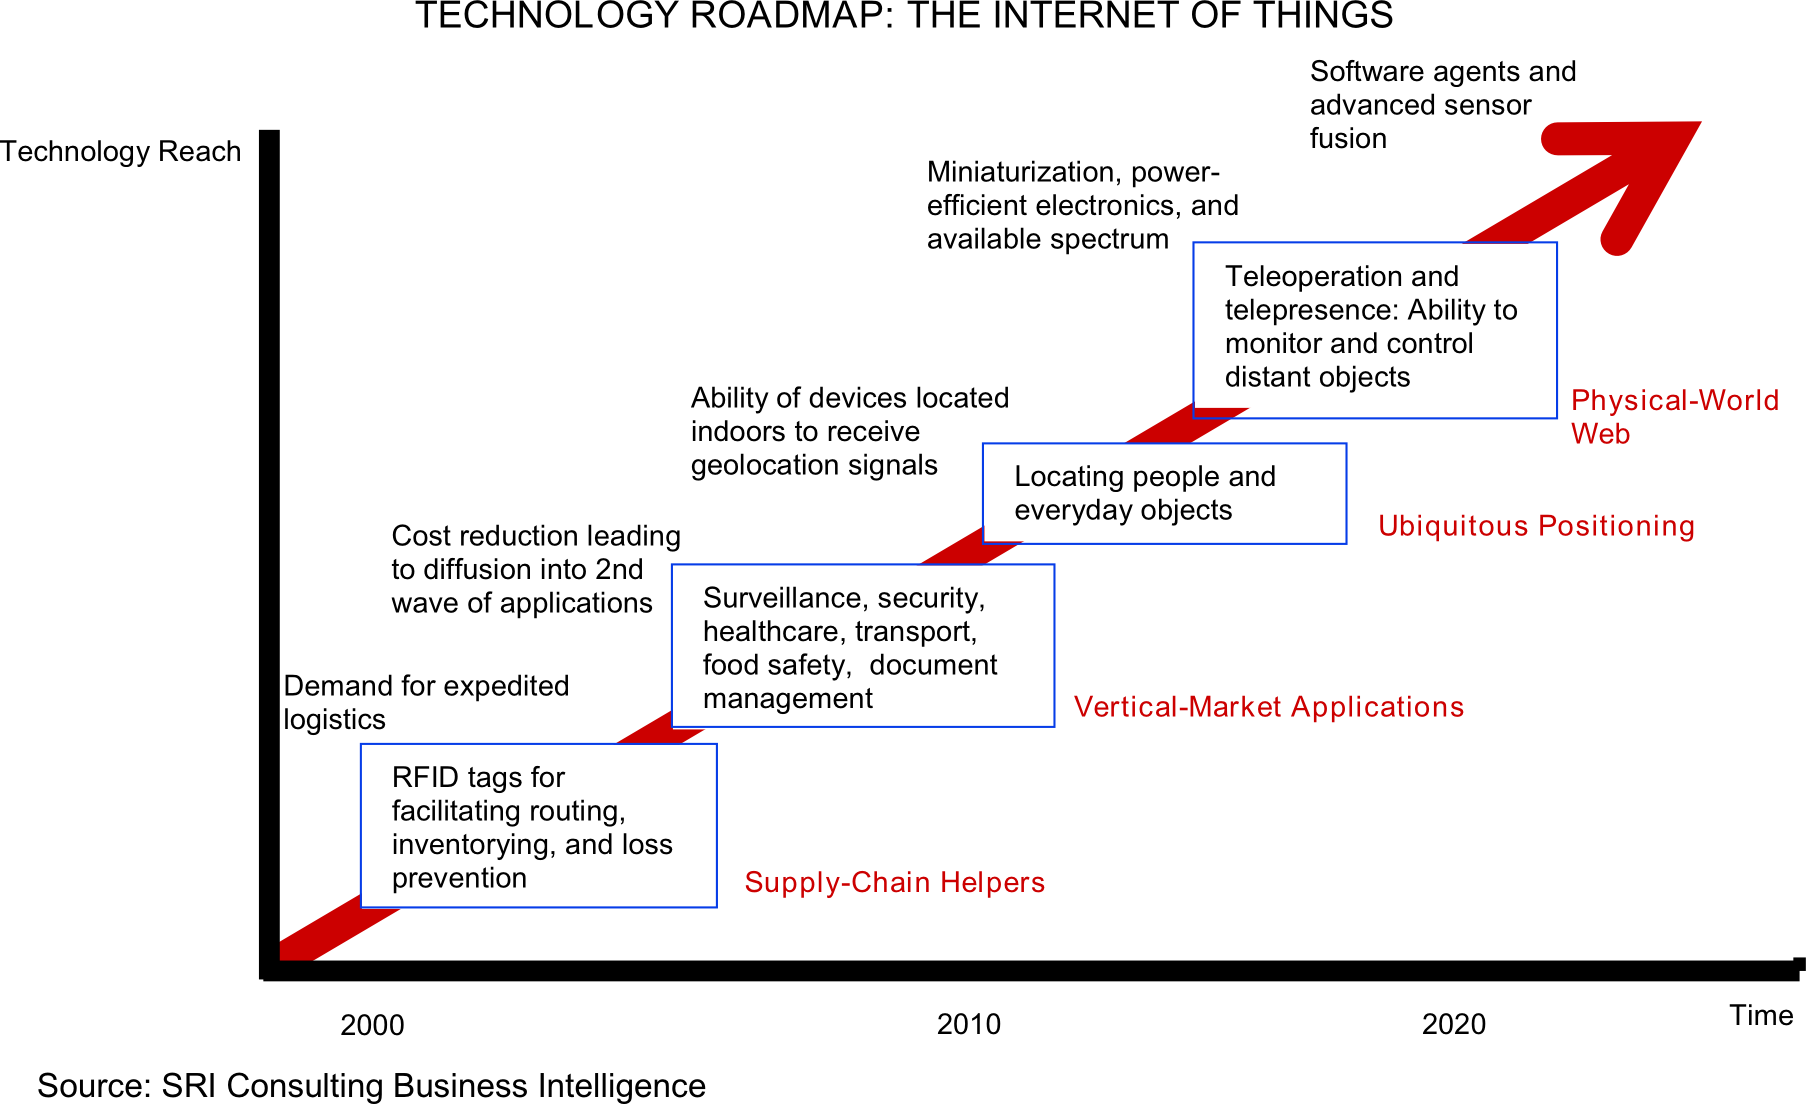
\includegraphics[width=\linewidth]{Internet_of_Things.png}
  \caption{Trend dell'internet of things}
  \label{fig:trendIoT}
\end{figure}
Secondo le proiezioni di Gartner, Inc. una corporation per la ricerca e advisory tecnologica, entro il 2020 ci saranno oltre 20 miliardi di device connesse all'Internet of Things. Si sta parlando di una Industria 4.0 dove l'automazione industriale integra l'IoT per migliorare le condizioni di lavoro e la produttivit\`a. La chiave di volta dell'Industria 4.0 sono i sistemi ciberfisici (CPS), ovvero sistemi fisici che sono strettamente connessi con i sistemi informatici e possono interagire e collaborare con altri sistemi CPS i quali costituiscono lo step evolutivo successivo delle device IoT. 
Un altro settore nel quale si proiettano ulteriori sviluppi \`e la Big Data Analysis. L'ubiquit\`a dei dispositivi intelligenti connessi all'Internet delle Cose permette analisi di dati vastissimi ai quali precedentemente era impensabile avere accesso. Le informazioni che si possono ricavare da questi dati sono molteplici e di sicuro interesse per molti ambiti di applicazione.

%% Interruzione di pagina
\newpage

%% Classi di applicazioni IoT
\section{Classi di applicazioni IoT}
Passiamo ora ad analizzare i campi di applicazione pi\`u diffusi per l'Internet delle Cose.

%% Qui ho rubato da Wikipedia inglese il paragrafo sulle Applications nella pagina dedicata all'IoT
%% TODO: Cambiare un po' le parole in modo che non si capisca che ho copiato =D
\subsection{Environmental monitoring}
Le applicazioni di monitoraggio ambientale tipicamente utilizzano sensori collegati all'Internet delle Cose per fornire assistenza nella protezione dell'ambiente. Il monitoraggio pu\`o interessare la qualit\`a dell'aria o dell'acqua, condizioni atmosferiche o del suolo, e pu\`o includere aree come il monitoraggio degli spostamenti della fauna selvatica e del suo habitat. Ci\`o pu\`o avere applicazioni anche nell'ambito della rilevazione di disastri naturali: sistemi di allerta per terremoti e tsunami possono essere implementati nell'ambito IoT. Device IoT in questo campo di applicazione sono tipicamente dislocate su un'ampia area geografica possono anche essere mobili.

\subsection{Infrastructure management}
Il monitoraggio e il controllo di infrastrutture urbane come ponti, rotaie, wind-farms \`e un campo di applicazione chiave dell'IoT. L'infrastruttura IoT pu\`o essere usata per monitorare eventi o cambiamenti nelle condizioni strutturali che possono compromettere la sicurezza o aumentare i rischi. Pu\`o altres\`\i\ essere usato per la programmazione di interventi di manutenzione in maniera pi\`u efficiente coordinando le operazioni tra diversi fornitori di servizi. Le device IoT sono anche usate per controllare infrastrutture critiche come ponti per fornire accesso alle navi. Si pensa che l'utilizzo di device IoT possa migliorare la gestione degli incidenti e la coordinazione in caso emergenze, la qualit\`a del servizia e ridurre i costi in tutte le aree legate alla gestione delle infrastrutture.

\subsection{Manufacturing}
L'ambiente manifatturiero \`e sicuramente una delle applicazioni di punta dell'IoT fina dalla sua nascita. Gli inteventi dell'IoT spaziano dalla gestione degli equipaggiamenti al tracking degli asset nell'ambiente produttivo. Questa sinergia permette alle aziende di avere una maggior flessibilit\`a e di ottimizzare in tempo reale i sistemi di produzione nonch\`e la rete di approviggionamento grazie all'interconnesione tra macchinari, sensori e sistemi.
L'integrazione di sistemi IoT all'interno di catene di produzione permette la predictive maintenance, valutazione statistica della degradazione dello stato dei macchinari, e prevenzione di guasti.
Come visto in precedenza l'evoluzione dell'Industria 4.0 \`e interamente basata sull'integrazione tra sistemi di produzione e l'Internet of Things.

\subsection{Energy management}
L'intregrazione di reti di sensori e attutatori, connessi ad internet, si pensa possa ottimizzare il consumo energetico in ambito industriale e casalingo. L'integrazione di device IoT all'interno di contatori per l'energia, cos\`\i\ come dispositivi domestici e industriali, capaci di comunicare con le compagnie per la rete elettrica possono permettere una gestione migliore della generazione ed utilizzo dell'energia. Questo tipo di device inoltre permetterebbe agli utenti di controllare in remoto i loro dispositivi, o controllarli centralmente grazie a interfacce cloud, in modo tale da implementare funzioni avanzate come la programmazione delle accensioni o dell'utilizzo dei dispositivi. Questo tipo di applicazioni \`e molto diffuso nel campo della domotica, i termostati IoT sono un ottimo esempio di questa applicazione.

\subsection{Medical and Healthcare}
Device connesse all'Internet delle cose possono essere abilitare il monitoraggio remoto dello stato di salute e sistemi di notifica delle emergenze. Queste device per il rilevamento dello stato di salute possono variare dal rilevamento della pressione arteriosa fino al conteggio dei battiti del cuore. Alcuni ospedali hanno cominciato ad utilizzare "letti smart" in grado di rilevare quanto il letto \`e occupato e quando il paziente sta cercando di alzarsi. Ormai sono molto diffusi dispositivi per il tracciamento delle attivit\`a dell'utente che incoraggiano uno stile di vita salutare, in questo ambito rientrano le wearable device come i fitness trackers.

\subsection{Settore dei trasporti}
%% Qui mi ricollego al PCN che \`e la sezione seguente
L'IoT pu\`o dare assistenza nella integrazione delle comunicazioni, controlli e elaborazione delle informazioni attraverso vari sistemi di trasporto. Le applicazioni dell'IoT si estendono a tutti gli aspetti dei sistemi di trasporto: i veicoli, l'infrastruttura, il pilota e i passeggeri. L'interazione dinamica tra questi componenti permette una comunicazione inter e intra veicolare, controllo del traffico intelligente, smart parking, gestione della logistica e delle flotte, controllo dei veicoli e sicurezza stradale.
L'applicazione sviluppata nel corso della tesi \`e appunto legata a questo ambito di applicazione dell'IoT e nel prossimo paragrafo ne analizzeremo gli obiettivi e funzionalit\`a.

%% Interruzione di pagina
\newpage

%% Sezione PCN
\section{Passenger Counter}
Il Passenger Counter, o contatore di passeggeri, \`e un dispositivo IoT la cui funzione \`e quella di rilevare e conteggiare i passeggeri presenti all'interno di un sistema di trasporto pubblico. Esso deve altres\`\i\ fornire i dati in tempo reale al gestore del servizio, sfruttando l'Internet delle Cose, in modo tale che sia possibile:
\begin{itemize}
\item Rilevare frodi.
\item Aumentare l'efficienza della flotta di mezzi migliorando la gestione e la programmazione dei percorsi.
\item Restringere il numero di persone sul mezzo per ragioni di sicurezza.
\item Analizzare i flussi di traffico all'interno delle citt\`a.
\end{itemize}
Il dispositivo deve essere in grado di effettuare il conteggio in modo non invasivo e contact-less, tenendo conto delle restrizioni dovute all'ambiente nel quale deve essere applicato.

\begin{figure}[h!]
  \centering
  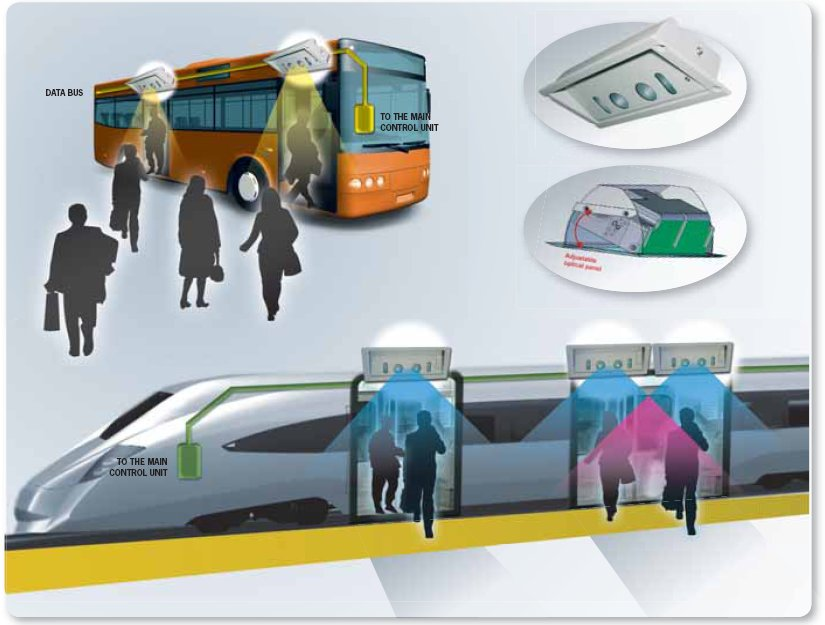
\includegraphics[width=9cm]{PassengerCountersz.jpg}
  \caption{Schematizzazione del contatore di passeggeri}
  \label{fig:SchemPCN}
\end{figure}

Il lavoro presentato in questa tesi \`e stato commissionato da Eurotech: azienda dedicata alla ricerca, sviluppo e produzione di sistemi embedded e computer ad alte prestazioni e con sede ad Amaro. L'azienda inoltre ha una forte rilevanza in ambito IoT in quanto, oltre a fornire dispositivi IoT ready, ha realizzato una piattaforma Machine-to-Machine che consente ai dispositivi, ai sensori e a tutti i sistemi distribuiti sul campo di comunicare tra loro trasferendo le informazioni rilevanti alle business application ed alle infrastrutture IT. Il PCN o Passenger Counter \`e uno dei prodotti di punta dell'azienda ed \`e stato selezionato come progetto per questa tesi.

%% Interruzione di pagina
\newpage

\begin{figure}[h!]
  \centering
  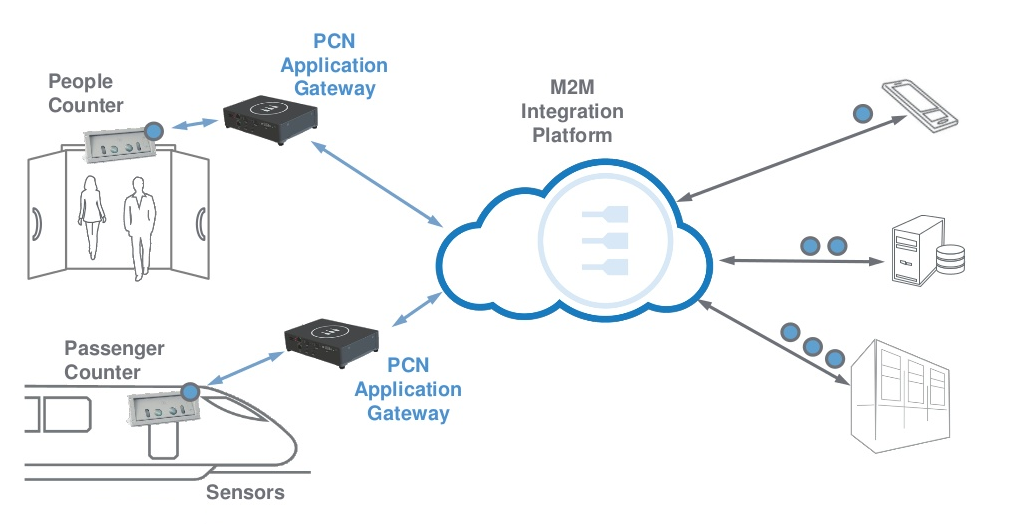
\includegraphics[width=\textwidth]{SchemaPCNIoT.png}
  \caption{Schema Passenger Counter Eurotech}
  \label{fig:SchemPCNEurotech}
\end{figure}

Il sistema di conteggio di passeggeri consta di tre parti fondamentali come schematizzato in figura \ref{fig:SchemPCNEurotech}:
\begin{enumerate}
\item Dispositivo di acquisizione video.
\item Dispositivo di elaborazione e trasmissione dei dati in real-time.
\item Infrastruttura di rete cloud per il raccoglimento dei dati.
\end{enumerate}
\`E quindi possibile accedere ai dati raccolti da pi\`u dispositivi per mezzo della piattaforma M2M proprietaria di Eurotech.

%% Interruzione di pagina
\newpage

\section{Obiettivi della tesi}
L'obiettivo della tesi \`e stato quello di realizzare una nuova versione del Passenger Counter di Eurotech basandosi sulla infrastruttura software/hardware fornita dall'azienda, cercando di migliorare quanto gi\`a fatto da Eurotech, esplorando soluzioni tecnologiche alternative. Questo obiettivo \`e stato quindi suddiviso in tre parti:
\begin{enumerate}
\item Identificare gli ambienti di sviluppo pi\`u idonei alla realizzazione del progetto.
\item Realizzare una nuova versione del Passenger Counter puntando a migliorare le prestazione ed abbattere i costi, adattandolo alle tecnologie usate dall'azienda per i suoi prodotti. 
\item Realizzare una infrastruttura software che fornisse tutti gli strumenti e le librerie necessarie all'implementazione del Passenger Counter realizzato e che potesse essere installato sulla piattaforma hardware fornita da Eurotech.
\end{enumerate}

% TODO: Attenzione! Aggiornare questa sezione ad ogni cambiamento della struttura del testo. (Se ce ne sono).
\section{Struttura della tesi}
Qui di seguito \`e riportata l'organizzazione del testo:
\begin{itemize}
\item Capitolo 1: Introduzione al contesto dell'Internet of Things e all'applicazione di conteggio dei passeggeri.
\item Capitolo 2: Analisi della versione corrente del Passenger Counter realizzato da Eurotech. Segue una trattazione dettagliata delle tecnologie e software utilizzati nella realizzazione del progetto.
\item Capitolo 3: Descrizione degli step intrapresi per lo sviluppo. Si suddivide in tre sezioni principali:
    \begin{itemize}
    \item Analisi degli ambienti disponibili per l'image processing embedded e motiviazioni per le quali si \`e deciso quello che \`e stato utilizzato.
    \item Implementazioni e confronti delle versioni realizzate per il contatore dei passeggeri.
    \item Realizzazione e features della distribuzione Linux realizzata a supporto del progetto
    \end{itemize}
\item Capitolo 4: Conclusioni
\end{itemize}

%% Capitolo 2: Contesto tecnologico di dettaglio
\chapter{Contesto tecnologico di dettaglio}
Passiamo ora a descrivere pi\`u tecnicamente e nel dettaglio le tecnologie utilizzare nello svolgimento della tesi.

\section{Tecnologie PCN Eurotech}

\begin{figure}[h!]
  \centering
  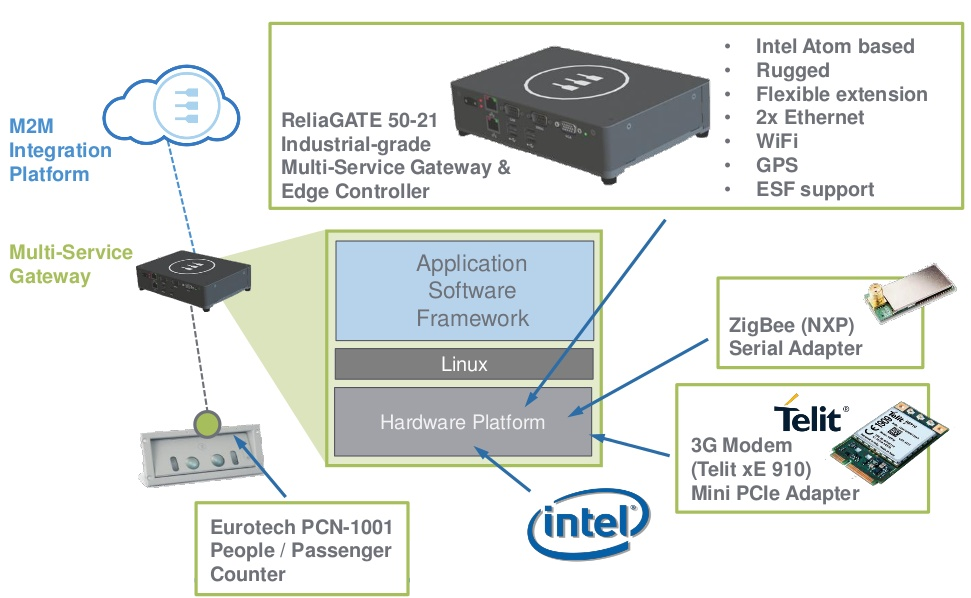
\includegraphics[width=\textwidth]{StrutturaPCN.png}
  \caption{Struttura del Passenger Counter di Eurotech}
  \label{fig:PCNEurotechHardware}
\end{figure}

%% Interruzione di pagina
\newpage

\subsection{Hardware}
Il sistema di conteggio dei passeggeri consta di due componenti hardware fondamentali: il gateway e il dispositivo di acquisizione delle immagini.

Il gateway \`e un'altro prodotto della Eurotech noto come ReliaGATE 50-21. Utilizza un processore x86 Intel Atom Z510P al quale sono state aggiunte opportune interfacce di rete per il deployment mobile. Esso ha infatti interfacce 2G/3G, WiFi, 802.15.4/Zigbee e GPS. Questo componente rappresenta l'unit\`a di elaborazione centrale del sistema nonch\`e il mezzo attraverso il quale i dati di conteggio vengono raccolti e trasmessi alla piattaforma cloud della Eurotech.

\begin{figure}[h!]
  \centering
  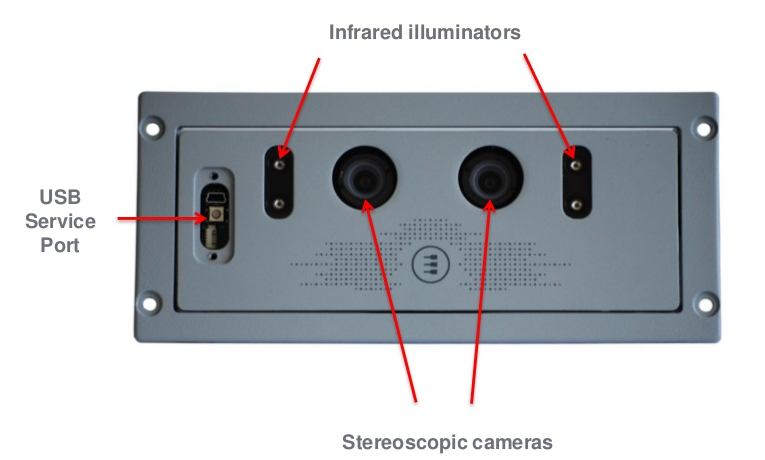
\includegraphics[width=\textwidth]{DispositivoAcquisizioneImmagini.png}
  \caption{Dispositivo di acquisizione delle immagini 3D}
  \label{fig:DispAcqImm3D}
\end{figure}

Il dispositivo di acquisizione video visibile in figura \ref{fig:DispAcqImm3D}. Esso nasconde al suo interno una FPGA programmata con una IP proprietaria Eurotech che permette la ricostruzione in 3D delle immagini acquisite dalle telecamere stereoscopiche di cui \`e dotato il dispositivo.
Il funzionamento \`e il seguente: i proiettori di luce infrarosse illuminano la scena, le telecamere a infrarossi stereoscopiche acquisiscono le immagini nello spettro della luce infrarossa. Le due immagini vengono passate alla FPGA che per mezzo di tecniche di ricostruzione stereoscopica accelerate in hardware permette di generare delle immagini in scala di grigi dove l'informazione di profondit\`a \`e data dal colore del pixel. Queste immagini vengono quindi passate all'unit\`a di elaborazione centrale che vi applica un semplice algoritmo per il tracciamento dei passeggeri di cui discuteremo il funzionamento nel dettaglio nel prossimo paragrafo.

%% Interruzione di pagina
\newpage

\subsection{Algoritmo per il tracciamento dei passeggeri}

\begin{figure}[h!]
  \centering
  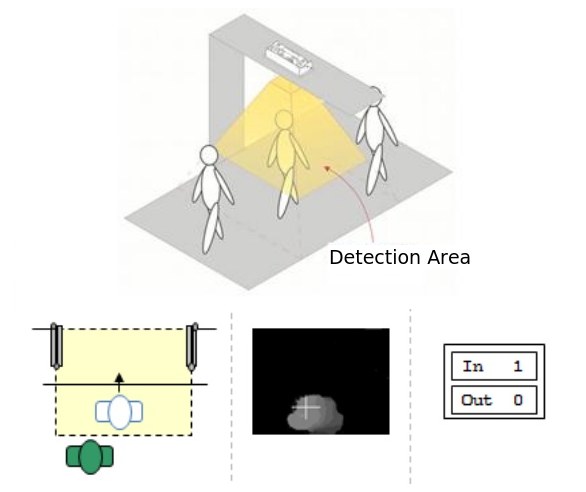
\includegraphics[scale=0.75]{Algoritmov2.png}
  \caption{Schematizzazione funzionamento algoritmo tracciamento passeggeri}
  \label{fig:SchemAlgrTrackPCNEurotech}
\end{figure}

%% TODO: Chiedere al prof se il conteggio viene effettuato sul ReliaGate o sul DynaPCN
L'unit\`a di elaborazione centrale si vede arrivare in ingresso una immagine in scala di grigi in cui \`e codificata l'informazione di profondit\`a tramite il colore dei pixel. I punti pi\`u vicini al rilevatore tendono al bianco, i punti pi\`u lontani tendono al nero.
Il cuore dell'algoritmo opera come segue:
\begin{enumerate}
\item Vengono rilevati i massimi locali all'interno dell'imagine in scala di grigi, i quali rappresentano le teste delle persone.
\item Traccia la posizione nel tempo di questi massimi locali all'interno del flusso di immagini.
\item Rileva quando questi massimi locali attraversano una linea di demarcazione virtuale, la quale indica l'ingresso o uscita dalla soglia e aggiorna i contatori.
\end{enumerate}
In figura \ref{fig:SchemAlgrTrackPCNEurotech} \`e riportata una schematizzazione di quanto accade durante il conteggio.

%% Interruzione di pagina
\newpage

\subsection{Infrastruttura software}

\begin{figure}[h!]
  \centering
  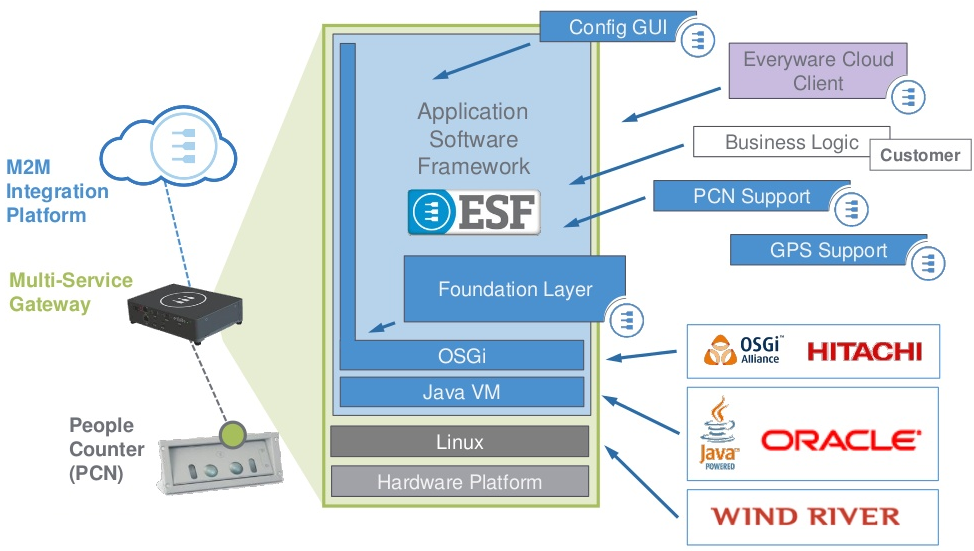
\includegraphics[width=\textwidth]{SoftwareStack.png}
  \caption{Schematizzazione stack software del sistema di Passenger Counting}
  \label{fig:StackSoftwarePCNEurotech}
\end{figure}

La piattaforma sulla quale si basa il Passenger Counter Eurotech \`e basata su una distribuzione custom di Linux realizzata per mezzo del progetto Yocto (Per affrondimenti circa questo strumento si veda il paragrafo \ref{Yocto}). Ad essa sono stati aggiunti i driver proprietari per le tecnologie Eurotech. Sopra di essa \`e presente la Java Virtual Machine la quale permette l'esecuzione del framework OSGi (Per affrondire questo framework si veda il paragrafo \ref{OSGi}). Su OSGi \`e basato il framework proprietario di Eurotech: Everyware Software Framework (ESF). Esso permette il deployment di applicazioni del cliente in modo flessibile tramite interfaccia grafica da web, la quale \`e resa disponibile dall'infrastruttura M2M di Eurotech.
Nei prossimi capitoli vedremo come sia stato necessario adattare l'applicazione realizzata nel corso di questa tesi alla infrastruttura qui descritta, nonch\`e modificare parte dell'infrastruttura per aggiungere funzionalit\`a mancanti e necessari alla nuova versione del Passenger Counter.

%% Interruzione di pagina
\newpage

\subsection{Problematiche di questa soluzione}
Questo sistema di conteggio dei passeggeri non \`e per\`o esente da problematiche, le quali sono state il punto di partenza per il mio lavoro. Le principali sono le seguenti:

\begin{enumerate}
\item Le ottiche del dispositivo di acquisizione delle immagini sono costose e difficili da reperire.
\item L'utilizzo di una FPGA per la ricostruzione delle informazioni di profondit\`a fa aumentare i costi di produzione.
\item Per come \`e stata implementata la soluzione \`e necessario installare una unit\`a computazionale per dispositivo di acquisizione delle immagini. Anche questo contribuisce ad aumentare i costi di produzione di un sistema PCN.
\end{enumerate}

Vedremo che nella versione del Passenger Counter realizzata nel corso di questa tesi sono stati risolti in buona parte tutte queste problematiche, con vari gradi di successo.

%% Interruzione di pagina
\newpage

\section{Tecnologie utilizzate durante lo sviluppo della tesi}
In questa sezione andremo ad esaminare le tecnologie che sono state utilizzate per realizzare la nuova versione del Passenger Counter.

%%TODO: Aggiungere nella bibliografia i riferimenti ai Datasheet delle telecamere
\subsection{Telecamere Intel RealSense}
Come dispositvi di acquisizione delle immagini sono state utilizzate le telecamere Intel RealSense. Esse sono telecamere ad infrarossi di nuova generazione che permettono la ricostruzione delle informazioni di profondit\`a della scena filmata sfruttando diverse tecniche di elaborazione delle immagini.

\subsubsection{Intel RealSense R200}

\begin{figure}[h!]
  \centering
  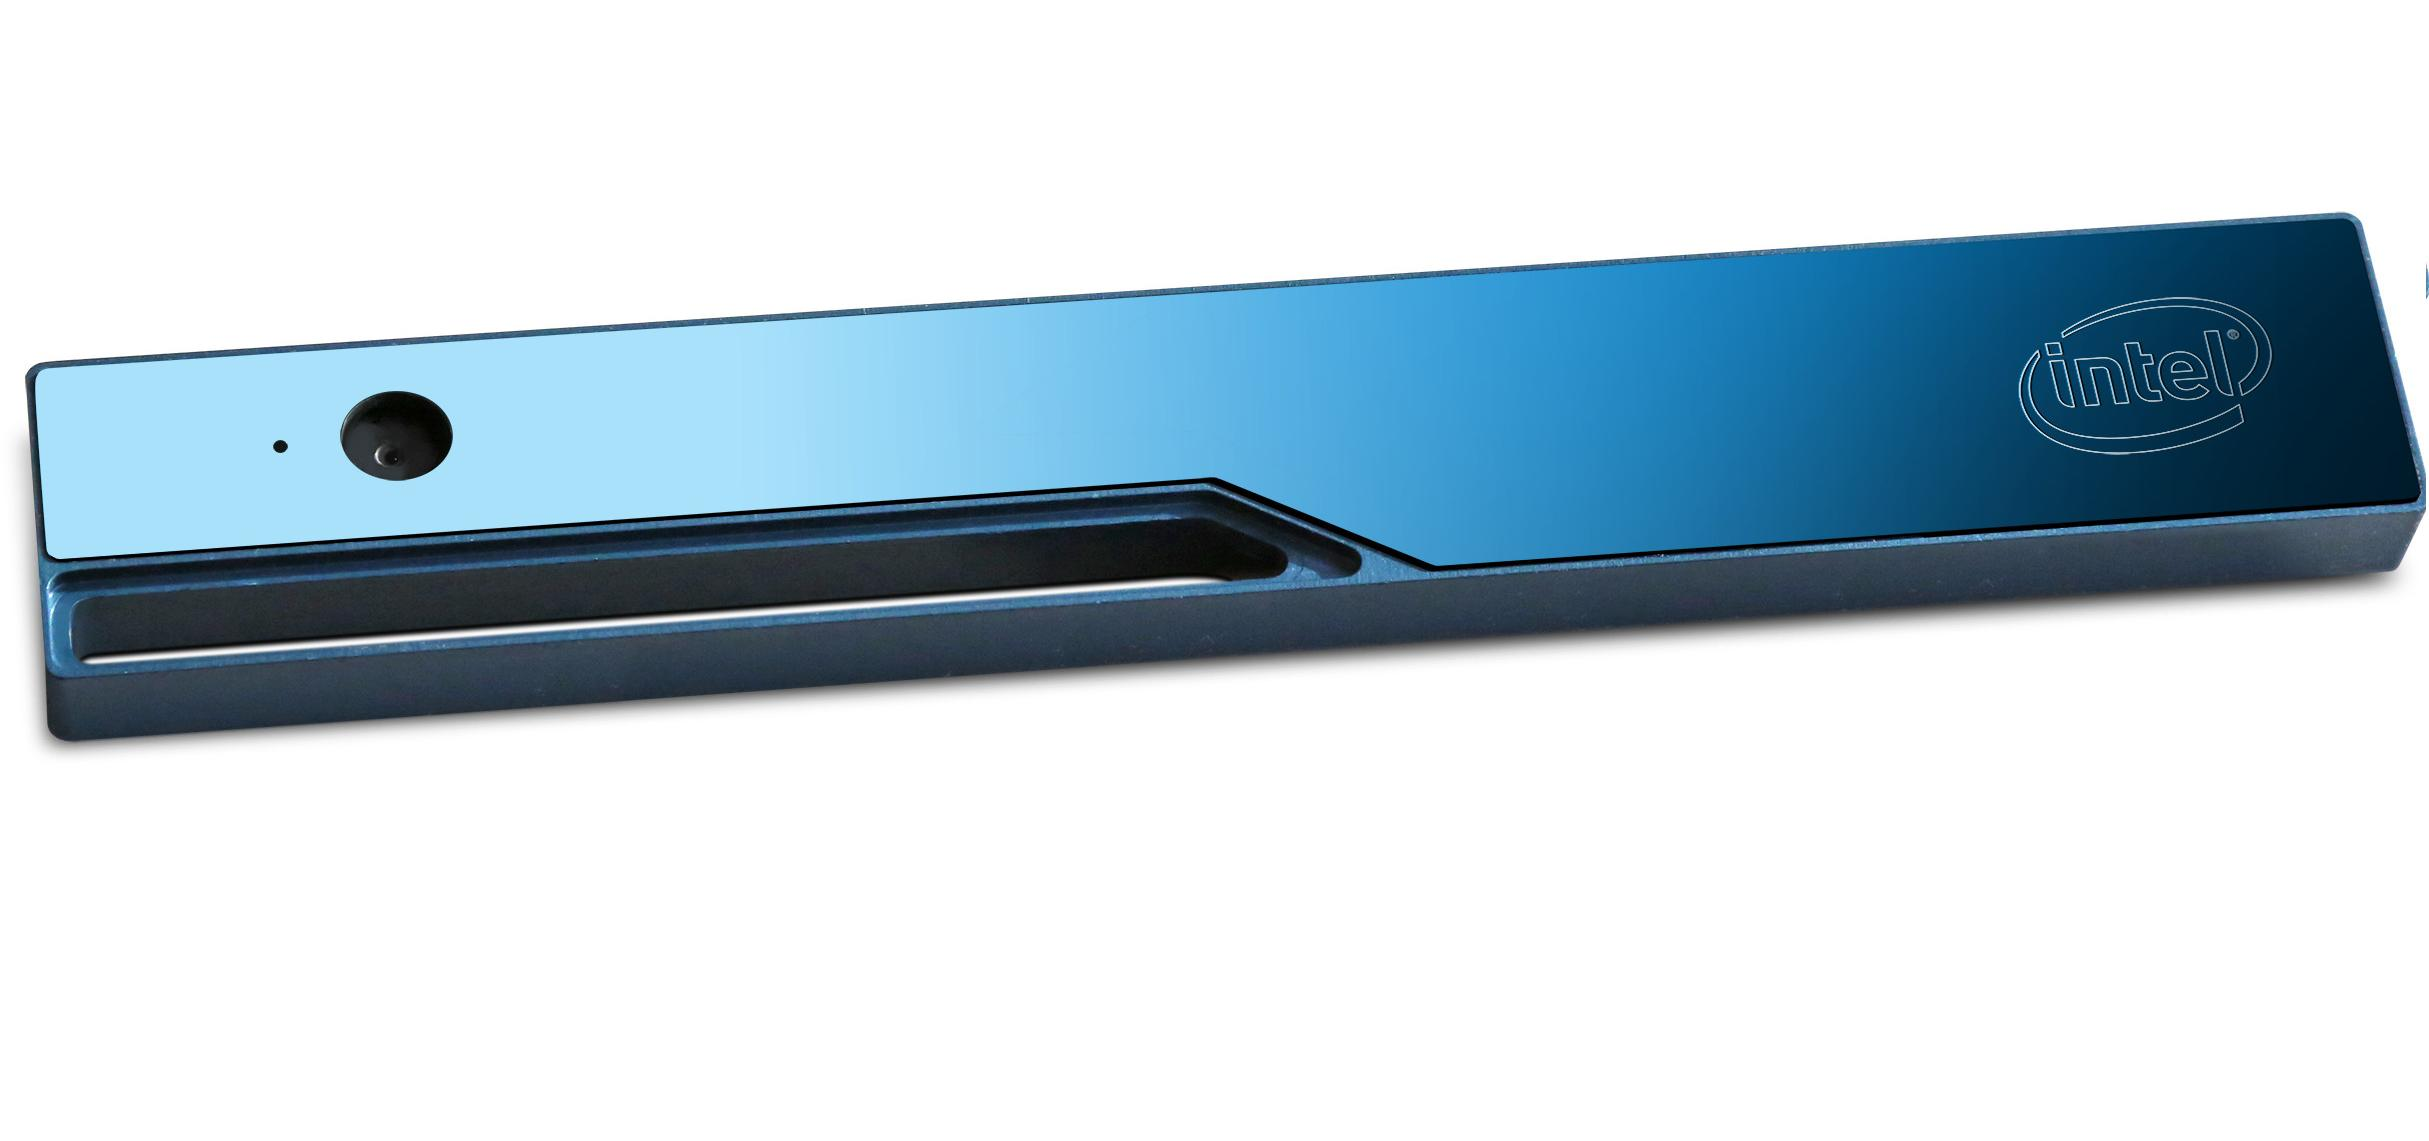
\includegraphics[width=.49\textwidth]{R200.jpg}
  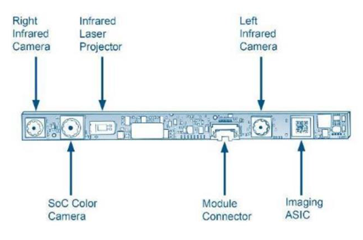
\includegraphics[width=.49\textwidth]{r200_module.png}
  \caption{Telecamera R200}
  \label{fig:R200}
\end{figure}

Il funzionamento di queste telecamere \`e lo stesso del Passenger Counter Eurotech. Sul modulo sono presenti due illuminatori ad infrarossi che illuminano la scena. Due telecamere stereoscopiche acquisiscono due immagini leggermente diverse dovute al diverso posizionamento delle telecamere. Analizzando le differenze tra le due immagini per mezzo di algoritmi di image processing ricostruiscono l'informazione di profondit\`a. Per ottenere una ricostruzione delle informazioni in real-time \`e stato usato un circuito ASIC che garantisse le prestazioni desiderate. Il funzionamento \`e riassunto in figura \ref{fig:SchemaFunzR200}.

\begin{figure}[h!]
  \centering
  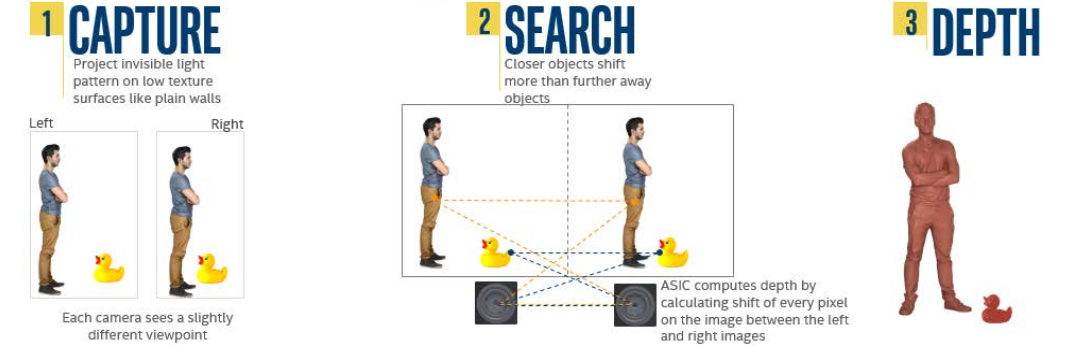
\includegraphics[width=\textwidth]{DepthDataFlowR200.png}
  \caption{Schema funzionamento Intel RealSense R200}
  \label{fig:SchemaFunzR200}
\end{figure}

Specifiche tecniche:

\begin{table}[h!]
    \centering
	\begin{tabular}{|c|c|c|}
	\hline
	& Depth Stream & Color Stream \\ \hline
	Risoluzione massima & 640 x 480 & 1920 x 1080 \\ \hline
    Frame rate massimo & 90fps & 60fps \\ \hline
    FOV (WxH) & 56 x 43 & 70 x 43 \\ \hline
    Indoor Range & 0.7 - 3.5m & - \\ \hline
    OutdoorRange & 10m & - \\
    \hline
	\end{tabular}
    \caption{Specifiche tecniche Intel RealSense R200}
    \label{table:R200Spec}
\end{table}

%% Interruzione di pagina
\newpage

\subsubsection{Intel RealSense SR300}

\begin{figure}[h!]
  \centering
  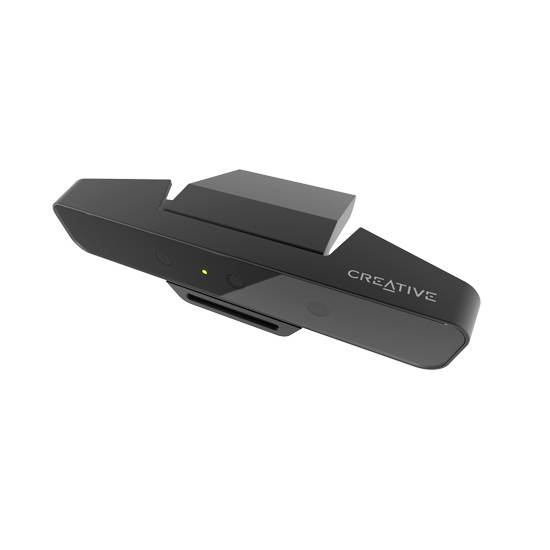
\includegraphics[width=.49\textwidth]{SR300.jpg}
  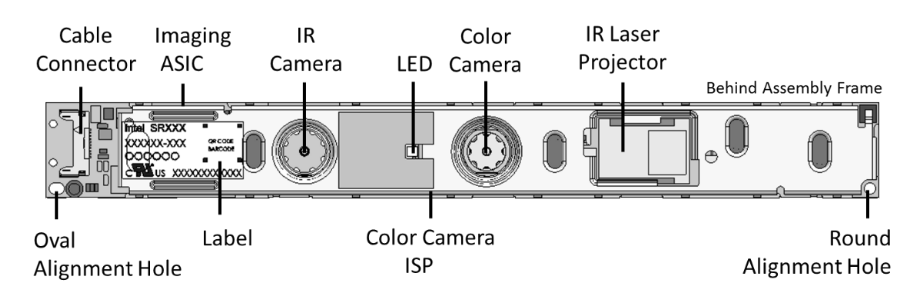
\includegraphics[width=.49\textwidth]{SR300_module.png}
  \caption{Telecamera SR300}
  \label{fig:SR300}
\end{figure}

La telecamera S300 utilizza una tecnica di rilevamento tridimensionale nota come luce strutturata. Il proiettore presente sul modulo proietta un pattern noto sulla scena. La deformazione dell'immagine proiettata permette ai sistemi di visione di calcolare la profondit\`a degli oggetti colpiti ed ottenere altre informazioni sulla superficio. L'acquisizione delle immagini a infrarossi in questo caso viene effettuata da un singolo scanner 3D a luce strutturata. In figura \ref{fig:SchemaFunzSR300} \`e schematizzato il funzionamento della telecamera.
Anche i questo caso l'informazione di profondit\`a viene ricostruita utilizzando un circuito ASIC.

\begin{figure}[h!]
  \centering
  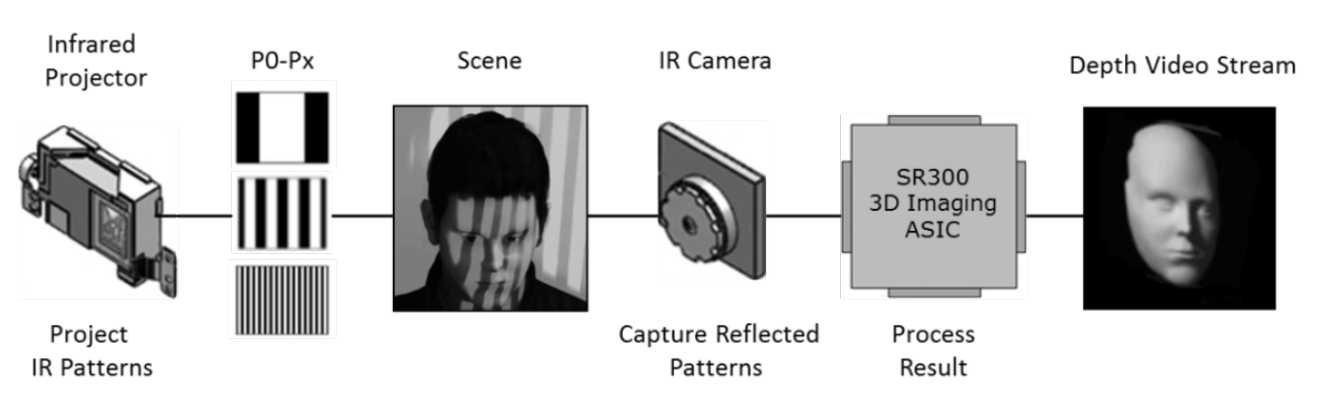
\includegraphics[width=\textwidth]{DepthDataFlowSR300.png}
  \caption{Schema funzionamento Intel RealSense SR300}
  \label{fig:SchemaFunzSR300}
\end{figure}

%% Interruzione di pagina
\newpage

Specifiche tecniche:

\begin{table}[h!]
    \centering
	\begin{tabular}{|c|c|c|}
	\hline
	& Depth Stream & Color Stream \\ \hline
	Risoluzione massima & 640 x 480 & 1920 x 1080 \\ \hline
    Frame rate massimo & 60fps & 60fps \\ \hline
    FOV (WxH) & 71 x 55  & 68 x 41 \\ \hline
    Indoor Range & 0.2 - 1.5m & - \\ \hline
    OutdoorRange & - & - \\
    \hline
	\end{tabular}
    \caption{Specifiche tecniche Intel RealSense SR300}
    \label{table:SR300Spec}
\end{table}

\subsubsection{Libreria librealsense e formato immagine}\label{librealsense}
Per l'interfacciamento software la Intel fornisce una libreria in C++ tramite la quale \`e possibile recuperare i frame dalle telecamere: la libreria \textbf{librealsense}\footnote{Repository libreria all'indirizzo: https://github.com/IntelRealSense/librealsense}. Essa provvede all'inizializzazione delle telecamere, apertura dei vari stream disponibili, impostazione di risoluzione e framerate. Gli stream disponibili sono: le immagini a colori, le immagini della telecamera a infrarossi e le immagini in cui \`e codificata l'informazione di profondit\`a. Nonostante usino tencologie diverse entrambe le telecamere forniscono lo stesso formato in uscita.

Lo stream di profondit\`a \`e uno stream di immagini a 16 bit privi di segno in cui il valore di ogni pixel rappresenta la distanza dalla telecamera. La distanza \`e fornita a meno di un fattore di scala reperibile per mezzo di una semplice chiamata di funzione. \`E possibile quindi risalire alla distanza in metri di un pixel dalla telecamera semplicemente moltiplicando il valore del pixel per il fattore di scala.
Vi \`e una eccezione a questa codifica in quanto, il valore del pixel 0, \`e attribuito ai pixel per i quali non \`e stato possibile ricavare informazione sulla distanza, ci\`o pu\`o essere dovuto a problemi di range o esposizione dell'immagine.

Vi sono per\`o delle minime differenze tra le due telecamere per quanto riguarda la risoluzione della distanza calcolata:
\begin{itemize}
\item Per la Intel RealSense SR300: il formato dello stream di profondit\`a \`e di 16 bit privi di segno interpolati su un range di 8m nonostante il range della telecamere arrivi ad un massimo di 1,5m. Ci\`o implica che la risoluzione della profondit\`a sia 0,125mm. 
\item Per la Intel RealSense R200: il formato \`e di 16 bit privi di segno interpolati su un range di circa 65m. Ci\`o implica una risoluzione di profondit\`a di 1mm.
\end{itemize}
Questo fatto non ha per\`o comportato problemi dal punto di vista della funzionalit\`a dell'applicazione in quanto la risoluzione e precisione delle telecamere non \`e critica per il corretto funzionamento del contatore.

%% Interruzione di pagina
\newpage

%% Copiato spudoratamente dalla mia presentazione su OpenCV.
\subsection{Libreria per l'image processing: OpenCV}\label{OpenCV}
Siccome una parte centrale della tesi verteva sull'elaborazione delle immagini \`e stato necessario integrare nel progetto l'uso della libreria OpenCV, ormai standard de facto nell'ambito dell'elaborazione delle immagini.

OpenCV, acronimo di Open Source Computer Vision, \`e una libreria software multipiattaforma finalizzata all'image processing real-time e alla computer vision. La libreria \`e rilasciata tramite licenza Berkeley Software Distribution (BSD) quindi \`e ad uso gratuito sia per fini accademici che commerciali. Contiene pi\`u di 2500 algoritmi pre-ottimizzati per le operazioni di image processing, comupter visione e machine learning pi\`u comuni. Sviluppata in C/C++, \`e dotata di interfacce verso C, Python, Java e MATLAB. Poich\`e finalizzata all'utilizzo real-time, la libreria sfrutta molteplici interfacce per l'accelerazione hardware (CUDA, OpenCL, Intel Integrated Perfomance Primitives). OpenCV ha una struttura modulare, il che significa che il pacchetto include diverse librerie statiche o condivise.

\subsubsection{Moduli principali e finalit\`a}
\begin{itemize}
\item \textbf{Modulo core}: funzionalit\`a di base. Lo scopo del modulo \`e  definire interfacce e funzionalit� che permettano di semplificare la manipolazione di immagini e flussi video. Il modulo contiene le funzionalit� di  base delle libreria e ne definisce le strutture fondamentali nonch\'e gestisce la memoria. 
\item \textbf{Modulo highui}: High-level GUI e Media I/O. l modulo HighGUI \`e stato progettato per fornire funzioni che permettano di provare le funzionalit\`a della libreria ed osservare i risultati velocemente. Fornisce semplici interfacce per creare e manipolare finestre che possano visualizzare immagini e aggiungere slider alle finestre, gestire semplici eventi come click del mouse e comandi da tastiera.
\item \textbf{Modulo imgproc}: image processing. Il modulo di Image Processing contiene funzioni e classi per la manipolazione di immagini. Ci\`o comprende:
    \begin{itemize}
    \item Image Filtering: funzioni per la convoluzione di immagini con un kernel, dilatazione di immagini, filtro Sobel, GaussianBlur ecc...
    \item Trasformazioni geometriche: ridimensionamenti, warping ecc...
    \item Funzioni per il disegno: permettono di disegnare semplici forme sulle immagini che vengono manipolate
    \item Funzioni per l'analisi delle immagini: istogrammi, analisi strutturale e descrittori di forme, motion analysis e tracking di oggetti.
    \end{itemize}
\item \textbf{Modulo videoio}: lettura e scrittura di file, nonch\`e analisi di video. Le funzioni principali implementate sono: analisi del movimento, sottrazione del background, rilevamento e tracciamento di oggetti.
\item \textbf{Modulo objdetect}: rilevazione di oggetti. Implementa funzioni e classi per il rilevamento e tracciamento di oggetti all'interno di immagini e flussi video. OpenCV ottiene tutto ci\`o facendo leva sui Haar Feature-based Cascade Classifier e Histogram of Oriented Gradients object detector.
\item \textbf{Modulo ml}: machine learning. La Machine Learning Library (MLL) \`e un insieme di classi e funzioni per la classificazione statistica, regressione e clustering dei dati. La maggior parte degli algoritmi di classificazione e regressione sono implementati come classi C++. Algoritmi implementati dal modulo:
    \begin{itemize}
    \item Artificial Neural Networks / Multi-Layer Perceptrons.
    \item Tree Classifier.
    \item Expectation Maximization algorithm.
    \item K-nearest Neighbors model.
    \item Logistic Regression.
    \item Normal Bayes Classifier.
    \item Support Vector Machines (SVM).
    \item Random forest predictor.
    \item Sochastic Gradient Descent SVM classifier.
    \end{itemize}
\end{itemize}

La struttura fondamentale della libreria \`e l'oggetto Mat, il quale \`e usato come contenitore delle immagini. Esso \`e una classe C++ formata da due componenti principali
\begin{itemize}
\item L'header: contenente informazioni come la dimensione della matrice, il metodo usato per salvarla, l'indirizzo dove \`e salvata ed un puntatore alla matrice.
\item La matrice: contenente i valori dei pixel dell'immagine la cui dimensionalit\`a dipende dal metodo utilizzato per salvare l'immagine (B/N, RGB ecc...)
\end{itemize}
Questa struttura \`e la stessa per tutti i tipi di immagine, indipendentemente dal formato nella quale \`e salvata. Questa astrazione facilita notevolmente la manipolazione delle immagini in quanto ci si riconduce velocemente ad una matrice di pixel manipolabile questa conversione \`e garantita dal modulo imgcodecs, la quale funzione non \`e altro che recuperare i dati sui pixel dell'immagine sulla quale si sta lavorando e generare i metadati per il tipo Mat.

\subsubsection{Storia}
Lanciato ufficialmente nel 1999, il progetto OpenCV era parte di una iniziativa Intel finalizzata all'avanzamento delle applicazioni CPU-intensive che includeva ray tracing real-time e display 3D. Inizialmente le finalit\`a del progetto erano descritte come:
\begin{itemize}
\item Permettere l'avanzamento della computer vision fornendo non solo una libreria di codice open-source ma anche pre ottimizzato per costruire l'infrastruttura base di applicazioni di computer visione.
\item Condividere conoscenza sulla computer vision fornendo una infrastruttura comune sulla quale tutti gli sviluppatori potessero costruire.
\item Far avanzare le applicazioni commerciali basate sulla computer vision rendendo il codice portabile, ottimizzato per le performance.
\end{itemize}
Ad oggi il supporto al progetto \`e dato dall'organizzazione no-profit OpenCV.org, la quale mantiene uno sviluppatore e un sito per la documentazione. La libreria \`e ormai lo standard de facto per le applicazioni di computer vision e image processing, vista la sua diffusione e la community molto attiva.

Per lo sviluppo dell'applicazione di Passenger Counter la scelta di utilizzare questa libreria \`e stata quasi obbligata visto l'ottimo supporto e diffusione della libreria. Inoltre la vasta portabilit\`a e l'attenzione alle performance la rendono particolarmente adatto al caso embedded real-time.

%% Interruzione di pagina
\newpage

%% TODO: Rivedi cosa hai scritto e amplia ancora se riesci
\subsection{Ambiente di sviluppo per l'OS: Yocto Project}\label{Yocto}
Per integrare nella piattaforma target gli strumenti necessari al funzionamento dell'applicativo \`e stato necessario realizzare una distribuzione Linux customizzata adatta alle nostre esigenze. Per farlo \`e stato utilizzato il progetto Yocto, standard industriale de facto per realizzare distribuzioni Linux embedded.

Yocto Project \`e un insieme di strumenti open source finalizzati alla creazione di distribuzioni Linux per sistemi embedded, corredate da toolchain di cross-compilazione ed emulatori, che siano indipendenti dall'architettura hardware. Yocto Project \`e quindi un ombrello sotto il quale si raccolgono vari sotto-progetti volti allo sviluppo di sistemi Linux embedded.

Le architettura supportate dal progetto sono le pi\`u diffuse nell'ambito embedded: ARM, MIPS, PowerPC e x86/x86-64. Una parte fondamentale di questo progetto \`e il build system open source basato sull'architettura OpenEmbedded. Questa implementazione di OpenEmbedded \`e chiamata Poky.

OpenEmbedded \`e framework software usato per creare distribuzioni Linux embedded. Il build system \`e basato sulle ricette BitBake le quali sono degli script bash specializzati che automatizzano la compilazione e la installazione di pacchetti software. Le ricette BitBake consistono di un URL che punta alla sorgente del pacchetto software, dipendenze e opzioni di compilazione ed installazione. Durante il processo di build sono usate per tenere traccia delle dipendenze ed effettuare cross-compilazione dei pacchetti affinch\`e sia possibile installarli sulla target distribution. BitBake stesso \`e uno dei componenti fondamentali di Yocto Project: \`e un build automation software, ovvero un tool che legge dei metadati sottoforma di "ricette" ed esegue task in base a dette ricette.

\subsubsection{Componenti del progetto Yocto}
\begin{itemize}
\item OpenEmbedded: \`e un build framework per embedded Linux. Permette la creazione di distribuzioni Linux complete per sistemi immersi e offre un ambiente di cross-compilazione completo. Il build system \`e basato su ricette BitBake.
\item BitBake: \`e un build automation software, ovvero un tool che legge dei metadati sottoforma di "ricette" ed esegue task in base a dette ricette. \`e uno dei componenti fondamentali di Yocto Project.
\item Poky: \`e una reference distribution di Yocto Project. Contiene l'OpenEmbedded Build System(BitBake e OpenEmbedded) assieme a un insieme di metadati che permettono di cominciare a costruire la propria distribuzione Linux embedded customizzata.
\item Layers: il build system del progetto Yocto \`e composto da layer. I layer sono una collezione logica di ricette che rappresentano stack di applicazioni o Board Support Packaged (BSP). I BSP contengono i pacchetti e i driver fondamentali necessari per costruire una distribuzione Linux per una specifica board o architettura. Solitamente questi BSP sono mantenuti dai produttori dell'hardware e sono l'interfaccia tra l'OS e l'hardware che lo esegue.
\end{itemize}

%% Interruzione di pagina
\newpage

\begin{figure}[h!]
  \centering
  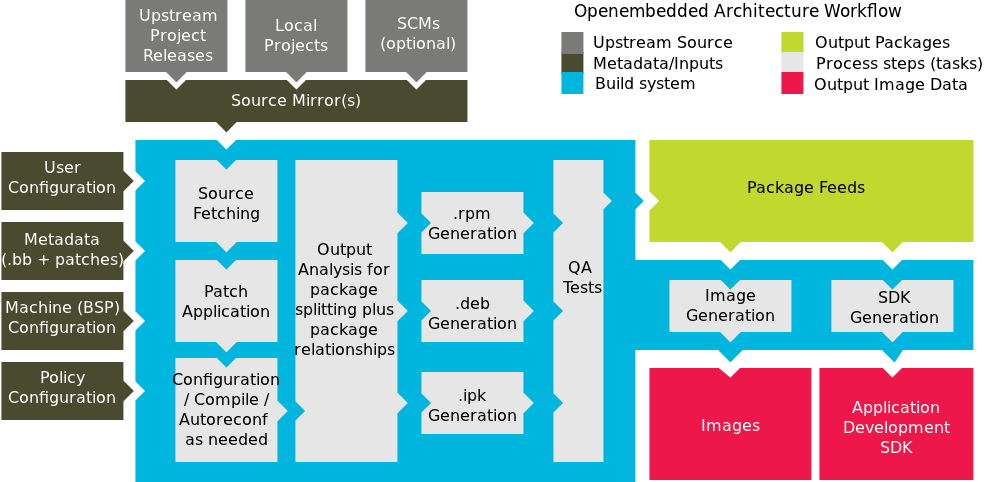
\includegraphics[width=\textwidth]{yocto-environment.png}
  \caption{Workflow progetto Yocto}
  \label{fig:WorkflowYocto}
\end{figure}

\subsubsection{Processo di build di una distribuzione}
Dopo aver configurato e lanciato il processo di build il build system provvede ad eseguire le seguenti operazioni per ogni pacchetto e applicazione che si desidera installare:
\begin{enumerate}
\item Recupera autonomamente i sorgenti remoti e locali.
\item Procede alla cross-compilazione dei sorgenti.
\item Genera i file .deb/.rpm/.ipk dipendentemente dalla configurazione.
\end{enumerate}
Una volta che sono stati generati tutti i pacchetti richiesti procede alla generazione dell'immagine della distribuzione, genera quindi il filesystem, installa i pacchetti e genera l'immagine che pu\`o essere eseguita sulla macchina target. In seguito \`e possibile generare la toolchain per la cross-compilazione di sorgenti per l'immagine della macchina target, questo processo generer\`a un piccolo installer il quale installer\`a la toolchain nella macchina dedicata allo sviluppo delle applicazioni per la piattaforma target.

%% Interruzione di pagina
\newpage

Per lo sviluppo dell'applicazione del Passenger Counter \`e stato necessario realizzare l'immagine della distribuzione Linux opportunamente modificata e la toolchain di cross-sviluppo prima di cominciare lo sviluppo dell'applicazione. Una volta completati questi passaggi si \`e potuti passare allo sviluppo dell'applicazione sulla SDKMachine. Siccome si \`e passati attraverso diverse tecnologie il processo \`e stato ripetuto pi\`u volte per poter integrare le nuove tecnologie all'interno della toolchain.

\begin{figure}[h!]
  \centering
  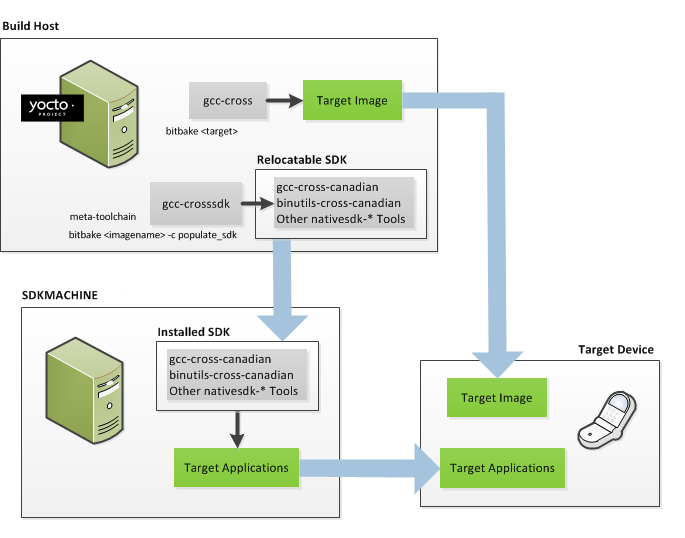
\includegraphics[scale=1]{cross-development-toolchains.png}
  \caption{Toolchain di cross-sviluppo del progetto Yocto}
  \label{fig:ToolchainYocto}
\end{figure}

%% Interruzione di pagina
\newpage

\subsection{Framework OSGi}\label{OSGi}
In pausa finch\`e non sei sicuro di usarlo.

% Capitolo 3: Corpo della tesi. Sviluppo del progetto: cosa ho fatto e come l'ho fatto.
\chapter{Sviluppo del progetto}
In questo capitolo verr\`a riportato come \`e stato affrontato lo sviluppo dell'applicazione e come sono stati affrontati i problemi riscontrati.

\section{Analisi degli ambienti di sviluppo disponibili per l'image processing embedded}
Nella fase iniziale del progetto si \`e studiato quale potesse essere l'ambiente di sviluppo adatto all'applicazione. Sono state considerate principalmente due possibilit\`a analizzate nei paragrafi seguenti.

\subsection{Ambiente di sviluppo Xilinx}

\begin{table}[h!]
    \centering
	\begin{tabular}{|c|c|}
	\hline
	Hardware & Avnet Zedboard \\ \hline
	Acquisizione video & HDMI Webcam \\ \hline
    Ambiente di sviluppo & Xilinx SDSoC \\ \hline
    Piattaforma software & Bare-metal\\
    \hline
	\end{tabular}
    \caption{Riassunto componenti ambiente di sviluppo Xilinx}
\end{table}

Inizialmente si era pensato usare una scheda di sviluppo Xilinx che integrasse una CPU ARM e una FPGA, in modo che fosse possible sfruttare i tool di sintesi di alto livello messi a disposizione da Xilinx per lo sviluppo. Utilizzando questo ambiente di sviluppo integrato sarebbe stato possibile realizzare applicazioni ad altissime prestazioni con la flessibilit\`a di un linguaggio ad alto livello come C/C++. Uno dei target di punta di questi sistemi di sviluppo \`e appunto l'image processing e come supporto forniscono anche librerie proprietarie pre-ottimizzate per l'hardware Xilinx.

%% Interruzione di pagina
\newpage

\subsubsection{Hardware}
La piattaforma target sarebbe stata una Avnet Zedboard.

Specifiche tecniche:

\begin{table}[h!]
    \centering
	\begin{tabular}{|c|c|}
	\hline
    ZYNQ-7000 SOC XC7Z020 & Dual-core ARM Cortex-A9 + FPGA Kintex-7 \\ \hline
    Memoria & 512 MB DDR3 + 256 Mb Quad-SPI Flash + 4GB SD card \\ \hline
    Espansione & FMC (Low Pin Count) + Pmod headers (2x6) \\ \hline
    Video & HDMI output (1080p60 + audio) + VGA \\
    \hline
	\end{tabular}
    \caption{Specifiche tecniche Avnet Zedboard}
\end{table}

Purtroppo, avendo la scheda una sola porta HDMI disponibile solo in output \`e stato necessario procurarsi un modulo aggiuntivo da collegarsi all'header FMC per avere a disposizione anche una porta HDMI in ingresso.

In figura \ref{fig:Zynq7000} \`e riportato il diagramma del SoC Zynq-7000.

\begin{figure}[h!]
  \centering
  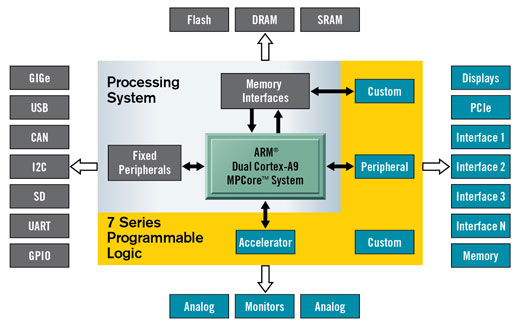
\includegraphics[width=\textwidth]{Zynq7000.jpg}
  \caption{Diagramma del SoC Zynq-7000}
  \label{fig:Zynq7000}
\end{figure}

%% Interruzione di pagina
\newpage

\subsubsection{Piattaforma per lo sviluppo SDSoC}
La piattaforma per lo sviluppo SDSoC permette uno sviluppo integrato dell'applicativo e dell'IP hardware utilizzando un linguaggio di alto livello come il C o il C++. Vista la maggiore familiarit\`a con i linguaggi di alto livello l'utilizzo di questo ambiente di sviluppo avrebbe comportato una maggior flessibilit\`a e velocit\`a nello sviluppo con il vantaggio di potersi avvalere dell'accelerazione hardware sfruttando la FPGA presente sul SoC.

\begin{figure}[h!]
  \centering
  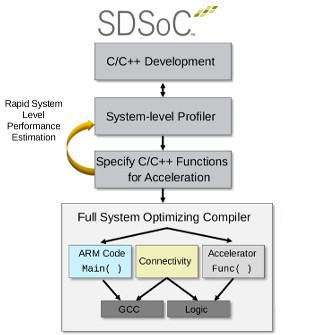
\includegraphics[scale=1]{XilinxSDSoC.png}
  \caption{Workflow SDSoC}
  \label{fig:SDSoC}
\end{figure}

SDSoC permette di scrivere l'intera applicazione in codice di alto livello. In fase di compilazione si va a specificare quale funzione si vuole eseguire sulla FPGA, per sfruttarne l'accelerazione hardware. A seguito dell'intervento del programmatore per specificare mappatura della memoria e ottimizzazioni per l'esecuzione in hardware, \`e possibile eseguire l'applicazione sull'ARM Cortex ed eseguire le task pi\`u pesanti dal punto di vista computazionale sulla FPGA.

%% Interruzione di pagina
\newpage

\subsubsection{Compatibilit\`a con OpenCV e liberia AuvizCV}

\begin{figure}[h!]
  \centering
  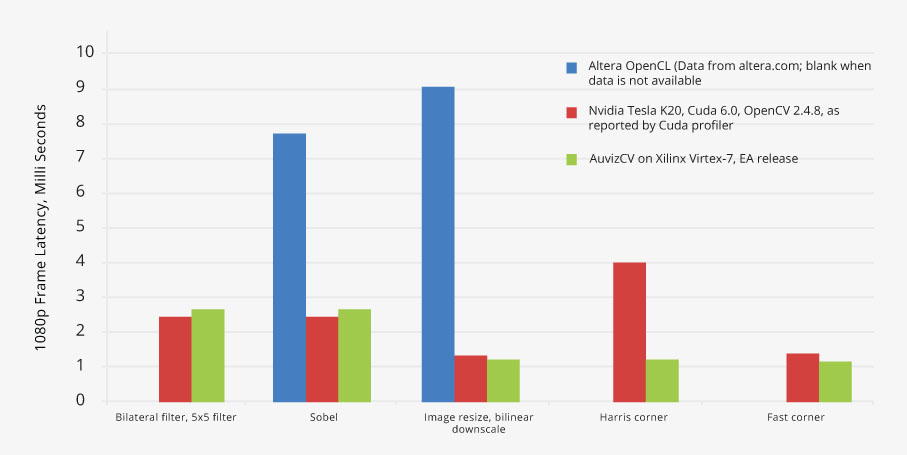
\includegraphics[width=\textwidth]{AuvizCV.jpg}
  \caption{Risultati benchmark}
  \label{fig:BenchmarkAuvizCV}
\end{figure}

Come ulteriore punto a favore di questo ambiente, Xilinx vantava la compatibilit\`a del sistema con OpenCV per l'esecuzione su CPU mentre rendeva disponibile una libreria compatibile con OpenCV per l'esecuzione su FPGA. Quest'ultima prende il nome di \textbf{AuvizCV}, la quale non \`e altro che un subset delle funzioni disponibili in OpenCV pre-ottimizzate per l'esecuzione sulle FPGA Xilinx. Questa libreria sfrutta le potenzialit\`a di SDSoC in quanto \`e stata scritta interamente in codice di alto livello e, in fase di compilazione, le funzioni utilizzate vengono sintetizzate sulla FPGA. Questa API si mantiene coerente con OpenCV per facilitare l'implementazione e l'accelerazione in harware. In figura \ref{fig:BenchmarkAuvizCV} sono riportati i risultati dei benchmark confrontando l'accelerazione di alcuni algoritmi di OpenCV usando varie tecnologie.

%% Interruzione di pagina
\newpage

%TODO: Approfondire?
\subsection{Ambiente di sviluppo Intel - Yocto}

\begin{table}[h!]
    \centering
	\begin{tabular}{|c|c|}
	\hline
	Hardware & Eurotech ReliaGate 20-25 \\ \hline
	Acquisizione video & Webcam - Telecamere Intel RealSense \\ \hline
    Ambiente di sviluppo & Toolchain generata con Yocto \\ \hline
    Piattaforma software & Distribuzione Linux custom Poky \\
    \hline
	\end{tabular}
    \caption{Riassunto componenti ambiente di sviluppo Intel - Yocto}
\end{table}

Come seconda possibilit\`a si \`e considerata la possibilit\`a di usare l'hardware reso disponibile da Eurotech e realizzare da zero l'infrastruttura software sfruttando il progetto Yocto.

\subsubsection{Hardware}
L'azienda ha fornito come piattaforma hardware un ReliaGate 20-25 nonch\`e le telecamere Intel RealSense.

\begin{figure}[h!]
  \centering
  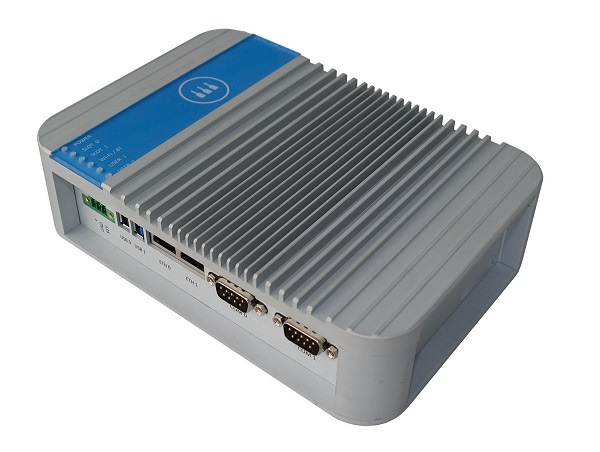
\includegraphics[scale=0.5]{ReliaGATE2025.jpg}
  \caption{ReliaGate 20-25}
  \label{fig:ReliaGate2025}
\end{figure}

Specifiche tecniche:

\begin{table}[h!]
    \centering
	\begin{tabular}{|c|c|}
	\hline
    ReliaGate 20-25-33 & Processore Intel E3827 Dual Core 1.75GHz x86-64 \\ \hline
    Memoria & 2GB 1333MHz DDR3L ECC + 8GB eMMC \\ \hline
    Connettivit\`a & 1x USB 3.0 + 2x USB 2.0 + 2x RS-232/RS-422/RS-485 \\ \hline
    Video & mini DisplayPort \\
    \hline
	\end{tabular}
    \caption{Specifiche tecniche ReliaGate 20-25-33}
\end{table}

\subsubsection{Software e piattaforma per lo sviluppo}
Gli strumenti che si sarebbe andati ad utilizzare sono quelli di cui si \`e parlato nel capitolo 2. Yocto per la realizzazione della distribuzione Linux, la toolchain di Yocto per la cross-compilazione dei sorgenti, OpenCV per l'image processing e le telecamere RealSense con annessa libreria.

%% Interruzione di pagina
\newpage

\subsection{Motivazioni per la scelta finale}
Si � infine scelto di utilizzare l'ambiente di sviluppo Intel - Yocto per i seguenti motivi:
\begin{itemize}
\item Flessibilit\`a: la possibilit\`a di aggiungere librerie e strumenti software grazie al progetto Yocto permetteva di avere un ambiente di lavoro molto pi\`u flessibile della controparte Xilinx.
\item Completezza: la libreria AuvizCV, seppur molto performante, mancava di moltissime funzioni rispetto ad una installazione completa di OpenCV, la quale poteva essere comodamente installata sul ReliaGate.
\item Performance: la CPU Intel \`e molto pi\`u performante dell'ARM presente sulla Zedboard. Siccome sarebbe stato comunque necessario eseguire parte del codice OpenCV sulla CPU, si sarebbero perse molte performance usando l'ambiente Xilinx.
\item Compatibilit\`a: anche se inizialmente non era previsto l'impiego delle telecamere RealSense, la board Xilinx non sarebbe potuta essere compatibile con queste ultime vista la mancanza di una porta USB 3.0 e il supporto software.
\end{itemize}

Nei prossimi capitoli procederemo con la descrizione del codice che \`e stato realizzato per la realizzazione del Passenger Counter.

%% Interruzione di pagina
\newpage

\section{Passenger Counter con sottrazione del background}
In questa sezione tratteremo la prima versione realizzata del contatore di passeggeri. Questa prima versione non faceva uso delle telecamere RealSense e presentava alcune criticit\`a che vedremo nel seguito. 

Inizialmente, descriveremo l'hardware utilizzato, tratteremo le tecniche utilizzate, quindi passeremo a descrivere la struttura del codice il suo funzionamento. Infine parleremo dei risultati ottenuti da questa implementazione e le problematiche principali.

\subsection{Componenti hardware}\label{HardwarePCN}
Per questa prima implementazione del contatore di passeggeri \`e stata utilizzata una semplice webcam.

\begin{table}[ht]
\begin{minipage}[b]{0.56\linewidth}
\centering
\begin{tabular}{ | c | c | }
    \hline
    Risoluzione & 640 x 480 \\ \hline
    Framerate & 30fps \\ \hline
	Connessione & USB 2.0 \\ \hline
    Tecnologia & driverless \\ \hline
    \end{tabular}
    \caption{Specifiche tecniche webcam}
    \label{table:SpecificheWebcam}
\end{minipage}\hfill
\begin{minipage}[b]{0.4\linewidth}
\centering
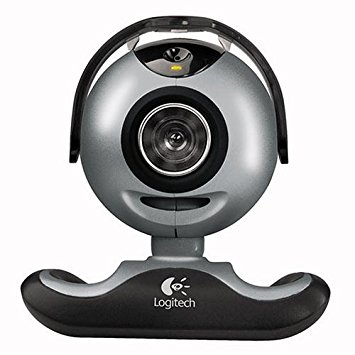
\includegraphics[width=40mm]{WebCam.jpg}
\captionof{figure}{Logitech QuickCam Pro 5000}
\label{fig:Webcam}
\end{minipage}
\end{table}

Essendo driverless veniva riconosciuta senza problemi dal ReliaGate ed \`e stato possibile leggere i frame in ingresso tramite OpenCV senza l'installazione di componenti software aggiuntivi.

% TODO: Approfondire? La matematica dietro il metodo \`e spiegata sufficientemente bene nella pagina di wikipedia
% link: 
\subsection{Algoritmo per la sottrazione del background}
La sottrazione del background \`e una tecnica, molto utilizzata dell'image processing e della computer vision, nella quale viene estratto il primo piano dell'immagine per essere ulteriormente manipolato. La background subtraction \`e una tecnica largamente utilizzata per rilevare soggetti in movimento all'interno di flussi video catturati da una telecamera statica.

L'algoritmo usato all'interno del codice di questa versione del contatore di passeggeri \`e basata su due paper pubblicati da Z.Zivkovic, "Improved adaptive Gausian mixture model for background subtraction" del 2004 e "Efficient Adaptive Density Estimation per Image Pixel for the Task of Background Subtraction" del 2006.

Questo algoritmo \`e anche noto come Gaussian Mixture-based Background/Foreground Segmentation Algorithm. Esso modella ogni pixel del background con una mixture di distribuzioni gaussiane selezionando automaticamente il numero appropriato da utilizzare. I pesi della mixture di gaussiane rappresentano il tempo per il quale quei colori permangono all'interno della scena. I colori che probabilmente appartengono al background sono quelli che rimangono per pi\`u tempo all'interno della scena e sono i pi\`u statici.

%% Interruzione di pagina
\newpage

Tipicamente, per facilitare l'elaborazione delle immagini a valle dell'applicazione dell'algoritmo di background subtraction, si ricava una immagine in scala di grigi nella quale i pixel neri rappresentano il background i pixel bianchi il primo piano. Nel caso dell'algoritmo usato per il Passenger Counter, le ombre vengono evidenziate con un colore grigio.
Qui di seguito \`e riportato un esempio di funzionamento.

\begin{figure}[h!]
  \centering
  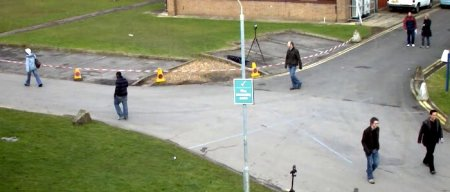
\includegraphics[width=.49\textwidth]{resframe.jpg}
  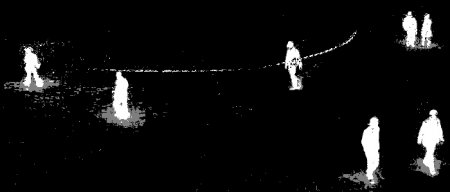
\includegraphics[width=.49\textwidth]{resmog2.jpg}
  \caption{Esempio funzionamento BackgroundSubtractorMOG2}
  \label{fig:EsempioBackSub}
\end{figure}

Questo algoritmo \`e reso disponibile dalla libreria OpenCV per mezzo della funzione BackgroundSubtractorMOG2. Nel seguito vedremo come \`e stato utilizzato all'interno del codice del Passenger Counter.

% TODO: Chiedere al prof quanto approfondire che qua \`e un casino leggersi il paper
\subsection{Algoritmo per il rilevamento dei contorni}
L'algoritmo \`e descritto in Suzuki, S. and Abe, K., Topological Structural Analysis of Digitized Binary Images by Border Following. CVGIP 30 1, pp 32-46 (1985).

Questo algoritmo per la rilevazione dei contorni \`e utilizzato anche nella seconda versione del Passenger Counter.

Qui di seguito \`e riportato un esempio di funzionamento.

\begin{figure}[h!]
  \centering
  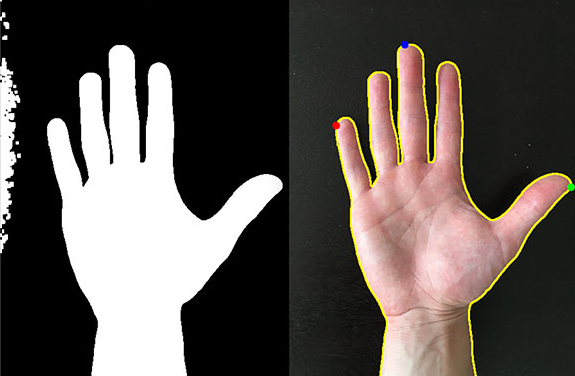
\includegraphics[scale=0.75]{findContours.png}
  \caption{Esempio funzionamento findContours: l'immagine a sinistra rappresenta l'immagine di input in bianco e nero ricavata dall'immagine a colori. L'immagine a destra \`e stata ricavata disegnando i contorni ricavati per mezzo dell'algoritmo sull'immagine a colori.}
  \label{fig:EsempioFindContours}
\end{figure}

%% Interruzione di pagina
\newpage

\subsection{Struttura del codice}

\begin{figure}[h!]
  \centering
  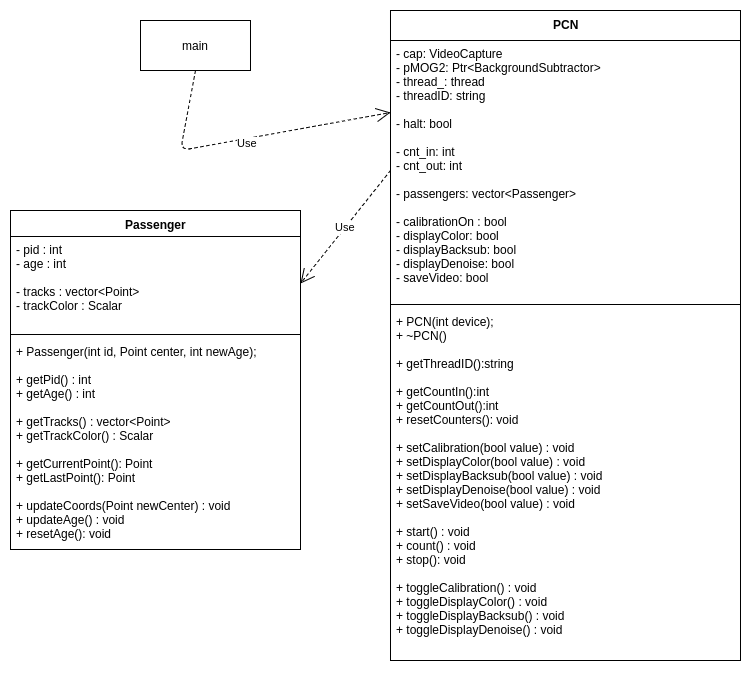
\includegraphics[width=\textwidth]{PCNUML.png}
  \caption{Diagramma UML del Passenger Counter a sottrazione del background}
  \label{fig:PCNUML}
\end{figure}

In figura \ref{fig:PCNUML} \`e riportata la struttura del programma. Le funzioni dei vari componenti del progetto sono le seguenti:
\begin{enumerate}
\item \textbf{Passenger}: la quale implementa la struttura adatta a rappresentare i passeggeri all'interno del programma.
\item \textbf{PCN}: la quale implementa il contatore di passeggeri vero e proprio. Questa implementazione permette la parallelizzazione dei contatori, \`e quindi possibile instanziare un contatore per telecamera.
\item \textbf{main}: implementa l'interfaccia utente per gestire i settaggi run-time dei PCN sfruttando i metodi pubblici resi disponibili dalla classe PCN.
\end{enumerate}

%% Interruzione di pagina
\newpage

\subsection{Classe Passenger}
Per il tracciamento dei passeggeri \`e stata creata una classe che contenesse le informazioni necessarie per il corretto tracking delle entit\`a.

\begin{lstlisting}[language=C++, caption=passenger.h]
class Passenger {

  public:

    // Constructor
    Passenger(int id, Point center, int newAge);

    // Selectors
    int getPid() {return pid;};
    int getAge() {return age;};

    vector<Point> getTracks(){return tracks;};
    Scalar getTrackColor(){return trackColor;};

    Point getCurrentPoint(){return tracks[tracks.size()-1];};
    Point getLastPoint(){return tracks[tracks.size()-2];};

    // Methods
    void updateCoords(Point newCenter);
    void updateAge(){age++;return;};

  private:
    int pid;    // Passenger ID
    int age;    // Passenger age

    vector<Point> tracks;
    Scalar trackColor;

};
\end{lstlisting}

\begin{lstlisting}[language=C++, caption=passenger.cpp]
Passenger::Passenger(int id, Point center, int newAge = 0)
{
    pid = id;
    age = newAge;

    tracks.push_back(center);
    int r = rand() % 255;
    int g = rand() % 255;
    int b = rand() % 255;
    trackColor = Scalar(r,g,b);
}

void Passenger::updateCoords(Point newCenter)
{
    tracks.push_back(newCenter);

    // If too many tracking points remove older points
    if(tracks.size() > MAX_TRACK_LENGTH) {
        tracks.erase(tracks.begin());
    }

    // Reset age
    // If the object is being tracked it means it's active we don't want it to disappear
    age = 0;

    return;
}
\end{lstlisting}

Questa classe ha tre obiettivi principali:
\begin{enumerate}
\item Identificare univocamente le entit\`a che entrano nel raggio visivo della telecamera.
\item Memorizzare lo storico delle posizione occupate da tali entit\`a all'interno del raggio visivo della telecamera.
\item Tenere traccia del tempo per il quale l'entit\`a rimane all'intenro del raggio visivo della telecamera.
\end{enumerate}

Queste necessit\`a sono state assolte per mezzo delle seguenti variabili:
\begin{enumerate}
\item \textbf{pid}: \`e un intero assegnato in fase di registrazione all'entit\`a-passeggero. Esso andr\`a ad identificarlo univocamente all'interno del programma.
\item \textbf{tracks}: \`e un vettore di coordinate che conservano la posizione dei passeggeri. Il massimo numero di posizioni mantenute in memoria \`e stato deciso sperimentalmente.
\item \textbf{age}: \`e un intero che va a rappresentare da quanto tempo il passeggero non viene rilevato nel raggio d'azione della telecamera. Oltre un certo valore di questo parametro il passeggero verr\`a rimosso dalla memoria del contatore.
\end{enumerate}

Inolte \`e stata implementata la variabile: \verb|trackColor|. \verb|trackColor| \`e un vettore di interi che vanno a rappresentare un colore RGB randomizzato. Viene usato per disegnare le tracce lasciate dal transito dei passeggeri nel raggio visivo della telecamera con colori diversi, in modo tale che sia facile verificare che il tracciamento sia avvenuto correttamente.

%% Interruzione di pagina
\newpage

\subsection{Classe PCN}

Questa classe ha come obiettivi principali:
\begin{itemize}
\item Implementare un oggetto contatore che fornisca interfacce verso l'esterno per poterne controllare i comportamenti.
\item Effettuare l'interfacciamento al dispositivo di acquisizione delle immagini.
\item Implementare il kernel del programma, ovvero la parte di codice incaricata di effettuare il conteggio degli attraversamenti della soglia da parte dei passeggeri sfruttando gli algoritmi di cui abbiamo parlato in precedenza.
\item Permettere l'esecuzione parallela di pi\`u contatori contemporaneamente, uno per telecamera collegata al unit\`a di elaborazione.
\item Permettere la visualizzazione e la registrazione dei risultati dell'elaborazione.
\end{itemize}

Qui di seguito \`e riportato l'header della classe PCN:
\begin{lstlisting}[language=C++, caption=PCN.h]
class PCN {

  public:

    PCN(int device);
    ~PCN() { thread_.join(); }

    // Selectors
    string getThreadID(){return threadID;};

    int getCountIn(){return cnt_in;};
    int getCountOut(){return cnt_out;};

    // Setters
    void setCalibration(bool value) {calibrationOn = value; return;};
    void setDisplayColor(bool value) {displayColor = value; return;};
    void setDisplayBacksub(bool value) {displayBacksub = value; return;};
    void setDisplayDenoise(bool value) {displayDenoise = value; return;};
    void setSaveVideo(bool value) {saveVideo = value; return;};

    // Methods
    void start();
    void count();
    void stop(){halt = true;};

    void resetCounters(){cnt_in = 0; cnt_out = 0; return;};

    void toggleCalibration();
    void toggleDisplayColor();
    void toggleDisplayBacksub();
    void toggleDisplayDenoise();

private:
    VideoCapture cap;
    Ptr<BackgroundSubtractor> pMOG2; //MOG2 Background subtractor

    std::thread thread_;
    string threadID;

    bool halt = false;

    // Passenger counters
    int cnt_in  = 0;
    int cnt_out = 0;

    // Passengers tracker
    int pid = 0;
    vector<Passenger> passengers;

    // Options
    bool calibrationOn = false;
    bool displayColor = false;
    bool displayBacksub = false;
    bool displayDenoise = false;
    bool saveVideo = false;
};
\end{lstlisting}

I punti rilevanti dell'header sono i seguenti:
\begin{itemize}
\item La funzione \verb|count()| rappresenta il kernel del programma e verr\`a analizzata in seguito.
\item Le funzioni toggle vengono usate per aprire e chiudere le finestre che visualizzano gli stream video nei quali sono riportati  i vari step dell'elaborazione dell'input.
\item La funzione \verb|toggleCalibration()| abilita la calibrazione real-time di alcuni parametri del kernel del programma. Questa calibrazione \`e resa possibile dal modulo HighGui di OpenCV il quale permette di aggiungere delle trackbar alle finestre video.
\item Il vettore di passeggeri rappresenta la memoria del contatore finalizzata al tracciamento dei passeggeri. Vedremo come verr\`a utilizzato nella funzione \verb|count()|.
\item \verb|cnt_in| e \verb|cnt_out| sono i contatori veri e propri, resi accessibili dall'esterno per mezzo dei selettori \verb|getCountIn()|, \verb|getCountOut()| e \verb|resetCounters()|.
\item \verb|thread_| e \verb|threadID| sono usati per la parallelizzazione del conteggio. Si noti che threadID viene usato per identificare univocamente le finestre degli stream video, questo si \`e reso necessario perch\`e OpenCV utilizza il nome delle finestre come identificatore e, nel caso di accesso a pi\`u telecamere contemporaneamente, ci\`o comportava problemi di non univocit\`a dei nomi e sovrapposizione di pi\`u stream in una stessa finestra.
\item \verb|pMOG2| implementa la sottrazione del background di cui abbiamo parlato in precedenza.
\end{itemize}

%% Interruzione di pagina
\newpage

\subsection{Analisi del kernel del programma: funzione count()}\label{kernelPCN}
La funzione \verb|count()| \`e il cuore del Passenger Counter. Ne suddivideremo il codice in tre sezioni principali:
\begin{enumerate}
\item Estrazione degli oggetti in movimento.
\item Rilevamento e tracking degli oggetti di nostro interesse.
\item Conteggio degli attraversamenti.
\end{enumerate}

\subsubsection{Estrazione degli oggetti in movimento}

\begin{lstlisting}[language=C++, caption=PNC.cpp metodo count() parte 1]
void PCN::count()
{
    // Streams
    Mat color;
    Mat fgMaskMOG2;
    Mat morphTrans;
    Mat denoisedMat;

    // Contours detection variables
    vector<vector<Point> > contours;
    vector<Vec4i> hierarchy;

    // Calibration
    int learningRate = LEARNINGRATE;
    int whiteThreshold = THRESHOLD;
    int dilateAmount = DILATE_AMOUNT;
    int erodeAmount = ERODE_AMOUNT;
    int blur_ksize = BLUR_KSIZE;
    int areaMin = AREA_MIN;
    int xNear = X_NEAR;
    int yNear = Y_NEAR;
    int maxPassengerAge = MAX_PASSENGER_AGE;

    while(!halt)
    {
        bool bSuccess = cap.read(color);

        pMOG2->apply(color, fgMaskMOG2, (float)(learningRate/10000.0));

        // --DENOISE
        // Threshold the image
        threshold(fgMaskMOG2, morphTrans, whiteThreshold, MAXRGBVAL, THRESH_BINARY);

        // Eroding
        erode(morphTrans,morphTrans, Mat(Size(erodeAmount,erodeAmount), CV_8UC1));

        // Dilating
        dilate(morphTrans,morphTrans, Mat(Size(dilateAmount,dilateAmount), CV_8UC1));

        // Blurring the image
        blur(morphTrans,morphTrans, Size(blur_ksize,blur_ksize));
        denoisedMat = morphTrans.clone();

        ...
    }
}
\end{lstlisting}

Il codice esegue le seguenti operazioni:
\begin{enumerate}
\item Anzitutto ci appoggiamo a OpenCV per andare a leggere i frame ricevuti dalla telecamera. Essi vengono direttamente convertiti in tipo \verb|Mat| per poter essere manipolati facilmente da OpenCV. Tutto questo \`e implementato dal metodo \verb|read()| della classe \verb|VideoCapture|.
\item I frame vengono passati alla funzione che applica la sottrazione del background. OpenCV prevede la creazione di un oggetto \verb|BackgroundSubtractor| il quale ha tra i suoi metodi l'applicazione della sottrazione del background. Questo metodo produce come output una immagine in scala di grigi nella quale i pixel bianchi appartengono al primo piano, i pixel neri appartengono al background, i pixel grigi alle ombre. Un parametro fondamentale della funzione \verb|apply()| \`e il \verb|learningRate|: esso rappresenta il peso con il quale viene aggiornato il modello del background.
\item Seguono delle trasformazioni  sui frame necessarie a minimizzare il rumore nell'immagine e semplificare il lavoro della funzione di rilevazione dei contorni.
    \begin{enumerate}
    \item Threshold: viene applicata una soglia per eliminare le ombre. Come abbiamo visto in precedenza l'algoritmo di sottrazione del background rileva le ombre e le colora di grigio. \`E possibile eliminarle imponendo una soglia che agisca sul colore dell'immagine. \verb|threshold()| fa in modo che ogni pixel il cui valore numerico \`e inferiore al valore dato come soglia (\verb|whiteThreshold|) viene portato al valore \verb|MAXRGBVAL| cio\`e 255. Ogni pixel che si trova sotto la soglia viene posto a 0. Ovvero:
    
    \begin{equation}
    dstPixel(x,y) = \begin{cases} MAXRGBVAL, & \mbox{se } srcPixel(x,y) > threshold \\ 0, & \mbox{altrimenti } \end{cases}
    \end{equation}

    Cos\`\i\ facendo le ombre, che hanno un colore il cui valore in pixel \`e inferiore al valore di soglia, vengono portate a zero e non vengono rilevate nei passaggi seguenti.
    \item Erosione: Questa operazione ha come risultato quello di espandere le regioni scure dell'immagine. L'obiettivo \`e quello di eliminare il rumore bianco gaussiano dall'immagine.
    \item Dilatazione: Questa operazione ha come risultato quello di far "crescere" le regioni luminose dell'immagine. L'obiettivo \`e quello di rendere pi\`u facilmente rilevabili gli oggetti del primo piano.
    \item Blur: Questa operazione effettua una sfocatura dell'immagine. L'obiettivo \`e sempre quello di ridurre il rumore dell'immagine. Questa funzione utilizza una semplice filtro lineare.
    \end{enumerate}
\end{enumerate}

%% Interruzione di pagina
\newpage

Risultato delle operazioni:

\begin{figure}[h!]
  \centering
  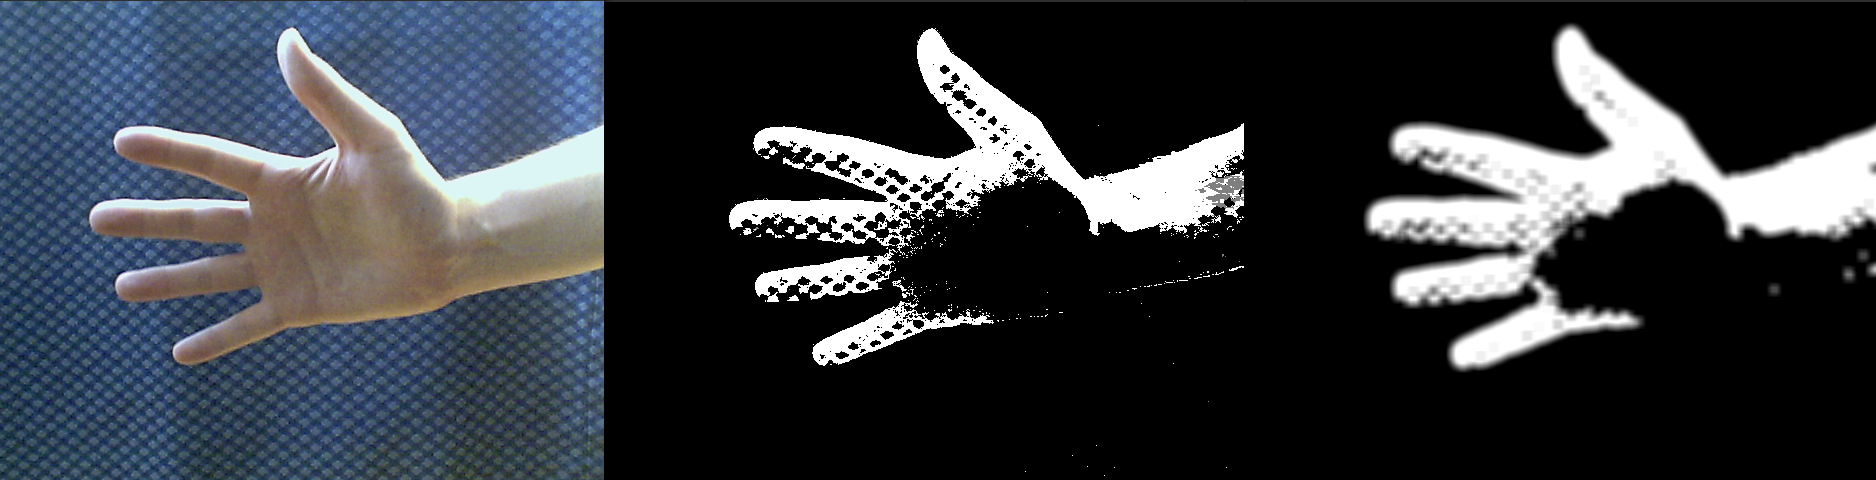
\includegraphics[width=\linewidth]{PCN1.png}
  \caption{L'immagine a sinistra rappresenta l'input. L'immagine al centro \`e il risultato dell'applicazione della sottrazione del background. L'immagine a destra \`e l'output delle operazioni di sottrazione del rumore.}
  \label{fig:PCN1}
\end{figure}

\subsubsection{Rilevamento e tracking degli oggetti di nostro interesse}

\begin{lstlisting}[language=C++, caption=PNC.cpp metodo count() parte 2]
while(!halt)
{
    ...

    // --FINDING CONTOURS
    findContours(morphTrans, contours, hierarchy, RETR_EXTERNAL, CHAIN_APPROX_NONE);

    // For every detected object
    for(unsigned int idx = 0; idx < contours.size(); idx++)
    {
        // -- AREA
        // Calculating area
        double areaCurrentObject = contourArea(contours[idx]);

        // If calculated area is big enough begin tracking the object
        if(areaCurrentObject > areaMin)
        {
            // Getting bounding rectangle
            Rect br = boundingRect(contours[idx]);
            Point2f mc = Point2f((int)(br.x + br.width/2) ,(int)(br.y + br.height/2) );

            // Drawing mass center and bounding rectangle
            rectangle( color, br.tl(), br.br(), GREEN, 2, 8, 0 );
            circle( color, mc, 5, RED, 2, 8, 0 );

            ...
        }

        ...
    }
}
\end{lstlisting}

%% Interruzione di pagina
\newpage

Il codice esegue le seguenti operazioni:

\begin{enumerate}
\item Ricava i contorni per mezzo della funzione di cui abbiamo discusso l'algoritmo nella sezione precedente.
\item Per ogni contorno completo rilevato dalla funzione eseguiamo le seguenti operazioni:
    \begin{enumerate}
    \item Ne calcoliamo l'area. Se supera una certa area minima, ricava sperimentalmente, decidiamo che si tratta di una persona.
    \item Ne ricaviamo il rettangolo che inscrive i controrni rilevati in precedenza tramite la funzione boundingRectangle.
    \item Di questo rettangolo rileviamo il centro.
    \item Per semplificare lo sviluppo e il debugging andiamo a disegnare questo rettangolo e questo centro sull'immagine a colori.
    \end{enumerate}
\end{enumerate}
L'informazione fondamentale per il resto dell'algoritmo \`e data dalla posizione del centro di questo rettangolo che rappresenter\`a la posizione dei passeggeri all'interno del raggio visivo della telecamera.

Risultato delle operazioni:

\begin{figure}[h!]
  \centering
  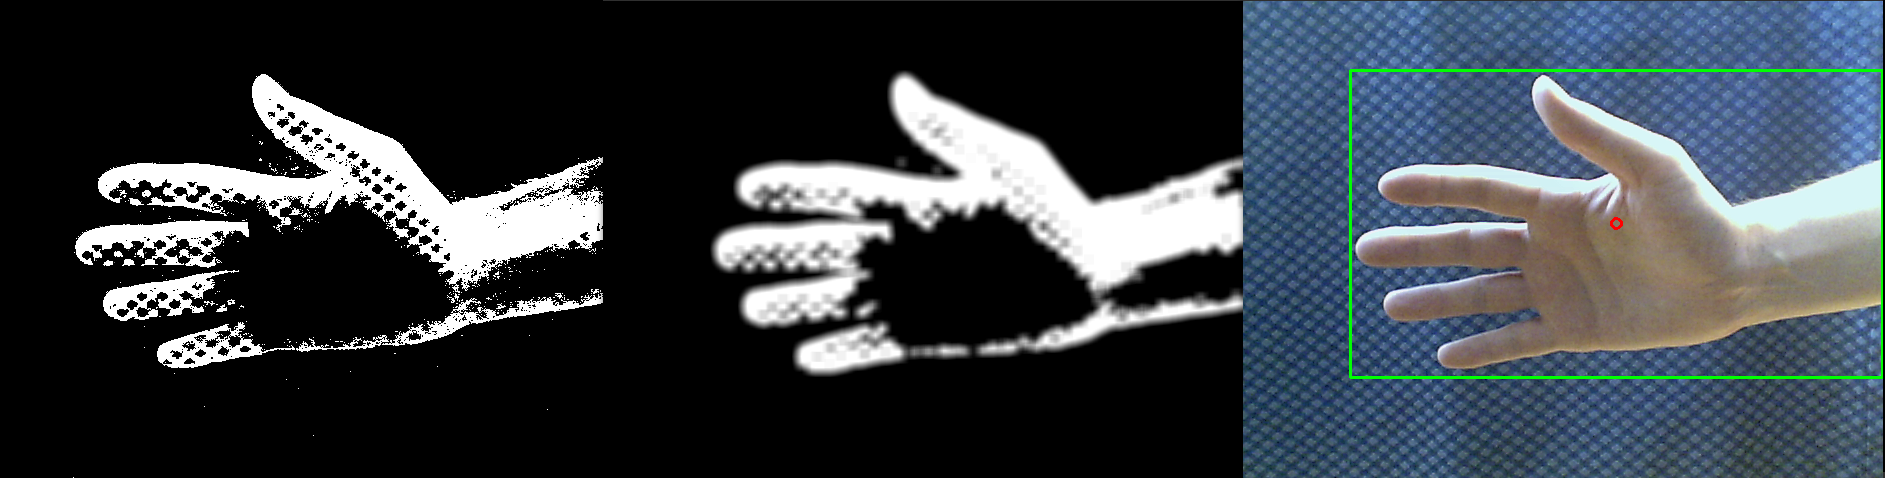
\includegraphics[width=\linewidth]{PCN2.png}
  \caption{L'immagine a sinistra rappresenta l'immagine in ingresso dopo la sottrazione del background. L'immagine al centro \`e l'output delle operazioni di sottrazione del rumore. L'immagine a destra \`e l'immagine di ingresso sulla quale sono stati disegnati il bounding rectangle e il centro del rettangolo.}
  \label{fig:PCN2}
\end{figure}

%% Interruzione di pagina
\newpage


\subsubsection{Conteggio degli attraversamenti}
Definiamo all'inizio del codice un vettore di passenger che rappresenter\`a il nostro database di passeggeri. Quindi il tracciamento di questi avverr\`a tramite il seguente codice.

\begin{lstlisting}[language=C++, caption=PNC.cpp metodo count() parte 3]
if(areaCurrentObject > areaMin)
{
    // Getting bounding rectangle
    Rect br = boundingRect(contours[idx]);
    Point2f mc = Point2f((int)(br.x + br.width/2) ,(int)(br.y + br.height/2) );

    // Drawing mass center and bounding rectangle
    rectangle( color, br.tl(), br.br(), GREEN, 2, 8, 0 );
    circle( color, mc, 5, RED, 2, 8, 0 );

    // --PASSENGERS DB UPDATE
    bool newPassenger = true;
    for(unsigned int i = 0; i < passengers.size(); i++)
    {
        // If the passenger is near a known passenger assume they are the same one
        if( abs(mc.x - passengers[i].getCurrentPoint().x) <= xNear &&
            abs(mc.y - passengers[i].getCurrentPoint().y) <= yNear )
        {
            // Update coordinates
            newPassenger = false;
            passengers[i].updateCoords(mc);

            // --COUNTER
            if(passengers[i].getTracks().size() > 1)
            {
                // Up to down
                if( (passengers[i].getLastPoint().y < color.rows/2 && passengers[i].getCurrentPoint().y >= color.rows/2) ||
                    (passengers[i].getLastPoint().y <= color.rows/2 && passengers[i].getCurrentPoint().y > color.rows/2) )
                {
                    // Counting multiple passenger depending on area size
                    if (areaCurrentObject > MAX_1PASS_AREA && areaCurrentObject < MAX_2PASS_AREA)
                        cnt_out += 2;
                    else if (areaCurrentObject > MAX_2PASS_AREA)
                        cnt_out += 3;
                    else
                        cnt_out++;

                    // Visual feedback
                    circle(color, Point(color.cols - 20, 20), 8, RED, CV_FILLED);
                }

                // Down to up
                if( (passengers[i].getLastPoint().y > color.rows/2 && passengers[i].getCurrentPoint().y <= color.rows/2) ||
                    (passengers[i].getLastPoint().y >= color.rows/2 && passengers[i].getCurrentPoint().y < color.rows/2) )
                {
                    // Counting multiple passenger depending on area size
                    if (areaCurrentObject > MAX_1PASS_AREA && areaCurrentObject < MAX_2PASS_AREA)
                        cnt_in += 2;
                    else if (areaCurrentObject > MAX_2PASS_AREA)
                        cnt_in += 3;
                    else
                        cnt_in++;

                    // Visual feedback
                    circle(color, Point(color.cols - 20, 20), 8, GREEN, CV_FILLED);
                }

            }

            break;
        }
    }

    // If it wasn't near any known object it is a new passenger
    if(newPassenger)
    {
        Passenger p(pid, mc);
        passengers.push_back(p);
        pid++;
    }
}
\end{lstlisting}

Il codice riportato esegue le seguenti operazioni:
\begin{enumerate}
\item Se l'entit\`a rilevata si trova entro una certa distanza massima da un passeggero che si trova all'interno del database assumiamo che siano lo stesso passeggero.
\item Di questo passeggero aggiorniamo la nuova coordinata e, nel caso abbia uno storico maggiore ad una singola coordinata, verifichiamo che non abbia superato la soglia virtuale rappresentata dalla met\`a del raggio visivo della telecamera. Il superamento della soglia \`e verificato come segue:
    \begin{itemize}
    \item Nel caso la penultima coordinata registrata si trovasse al di sotto della soglia visiva e l'ultima coordinata sopra, aggiorniamo il contatore degli ingressi.
    \item Nel caso la penultima coordinata registrata si trovasse al di sopra della soglia visiva e l'ultima coordinata sotto, aggiorniamo il contatore delle uscite.
    \end{itemize}
\item Nel caso l'entit\`a non si trovasse vicino a nessun passeggero noto si tratta di un nuovo passeggero appena entrato all'interno del raggio visivo della telecamera. Procediamo quindi ad aggiornare il database aggiungendo il nuovo passeggero.
\end{enumerate}

Per visualizzare quanto avviene all'interno del programma e semplificare il debugging tramite OpenCV si \`e deciso di plottare a schermo tutte le informazioni utilizzate nel codice precedente.
Questa parte di plot delle informazioni \`e stata implementata per mezzo del codice seguente:

\begin{lstlisting}[language=C++, caption=PNC.cpp metodo count() parte 4]
// For every passenger in passengers DB
for(unsigned int i = 0; i < passengers.size(); i++)
{
    // -- DRAWING PASSENGER TRAJECTORIES
    if(passengers[i].getTracks().size() > 1)
    {
        polylines(frame, passengers[i].getTracks(), false, passengers[i].getTrackColor(),2);
        putText(frame, "Pid: " + to_string(passengers[i].getPid()), passengers[i].getCenter(), FONT_HERSHEY_SIMPLEX, 0.5, passengers[i].getTrackColor(), 2);
    }

    // --UPDATE PASSENGER STATS
    // Updating age
    passengers[i].updateAge();

    // Removing older passengers
    // NB: The age depends on the FPS that the camera is capturing!
    if(passengers[i].getAge() > maxPassengerAge)
    {
        passengers.erase(passengers.begin() +i);
    }
}

// --PRINTING INFORMATION
putText(frame, "FPS: " + to_string(fps), Point(0,  15) , FONT_HERSHEY_SIMPLEX, 0.5, RED, 2);

putText(frame, "Count IN: "  + to_string(cnt_in), Point(0,frame.rows - 30) , FONT_HERSHEY_SIMPLEX, 0.5, WHITE, 2);
putText(frame, "Count OUT: " + to_string(cnt_out), Point(0, frame.rows - 10) , FONT_HERSHEY_SIMPLEX, 0.5, WHITE, 2);
\end{lstlisting}

Si noti che oltre a disegnare le tracce dei passeggeri, il ciclo for viene usato anche per aggiornare la variabile \verb|age| dei passeggeri. Quando questo parametro supera un certo valore di soglia, dovuto al fatto che i passeggeri sono usciti dal raggio visivo della telecamera da troppo tempo, vengono rimossi dal database.

%% Interruzione di pagina
\newpage

Risultato tracciamento in fase sperimentale. La linea rossa rappresenta la soglia per l'attraversamento.

\begin{figure}[h!]
  \centering
  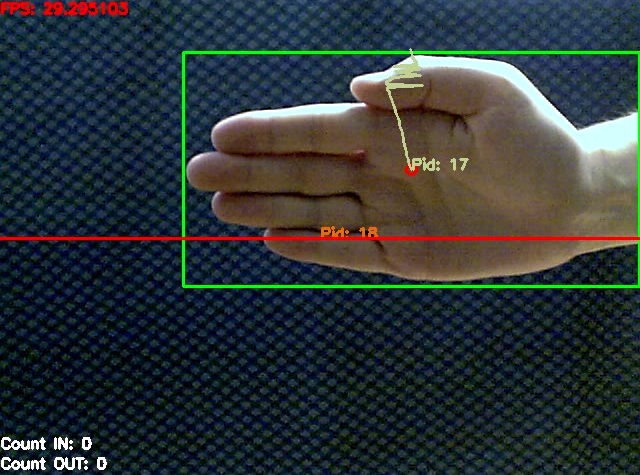
\includegraphics[scale=0.65]{PCNMano1.png}
  \caption{Risultato tracciamento sperimentale PCN. Frame precedente all'attraversamento.}
  \label{fig:PCNMano1}
\end{figure}

\begin{figure}[h!]
  \centering
  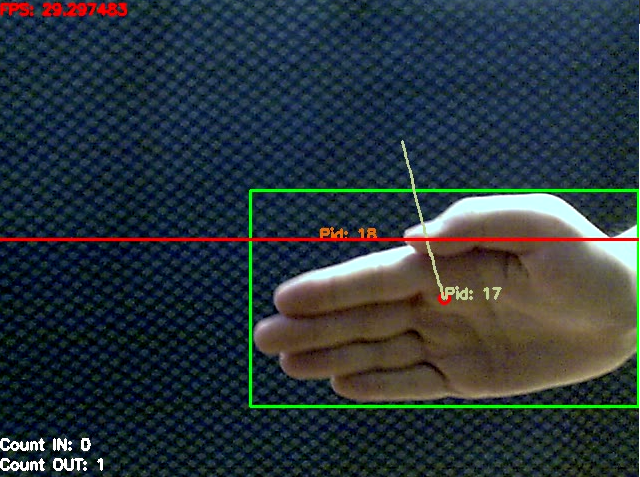
\includegraphics[scale=0.65]{PCNMano2.png}
  \caption{Risultato tracciamento sperimentale PCN. Primo attraversamento.}
  \label{fig:PCNMano2}
\end{figure}

%% Interruzione di pagina
\newpage

\begin{figure}[h!]
  \centering
  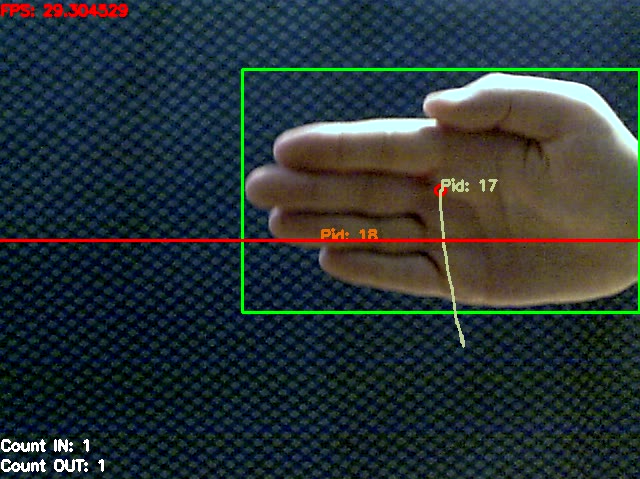
\includegraphics[scale=0.65]{PCNMano3.png}
  \caption{Risultato tracciamento sperimentale PCN. Secondo attraversamento.}
  \label{fig:PCNMano3}
\end{figure}

Dalla successione delle immagini si pu\`o notare come il tracciamento sia buono in condizioni ideali. Si noti che il punto al centro dello schermo \`e dovuto alla scomparsa di un oggetto rilevato dal raggio visivo della telecamera ma che non ha ancora superato il limite massimo di \verb|age|.

%% Interruzione di pagina
\newpage

\subsection{main.cpp}

\begin{lstlisting}[language=C++, caption=main.cpp]
int main(int argc, char * argv[])
{
    bool stop = false;
    bool displayHelpFlag = false;
    char choice;

    vector<PCN *> counters;

    for(int i = 0; i < deviceNumber; i++) {
        counters.push_back(new PCN(i));
        cout << endl; 
        cout << "Device number: " << i << endl;
    }

    if(argc >= 2)
    {
        if(!strcmp(argv[1], "-s")) {
            for(int i = 0; i < deviceNumber; i++) {
                counters[i]->setSaveVideo(true);
            }
        }
    }

    for(int i = 0; i < deviceNumber; i++) {
        counters[i]->start();
    }

    do
    {
        cout << "Please enter a valid command:\n>";
        choice = getchar();
        cout << "You entered: " << choice << endl;

        for(int i = 0; i < deviceNumber; i++) {
            
            cout << "Device : " << i << endl;
            switch(choice)
            {
                case('p'):
                    cout << "Current count:\n";
                    cout << "Count in  = " << counters[i]->getCountIn() << endl;
                    cout << "Count out = " << counters[i]->getCountOut() << endl;
                    cout << "Current balance =" << counters[i]->getCountIn() - counters[i]->getCountOut() << endl;
                    break;

                case('r'):
                    cout << "Resetting counters\n";
                    counters[i]->resetCounters();
                    break;

                case('c'):
                    cout << "Toggle color\n";
                    counters[i]->toggleDisplayColor();
                    break;
                
                ...
                
                case('q'):
                    cout << "Exiting program!\n";
                    counters[i]->stop();
                    cout << "Capture closed.\n";
                    stop = true;
                    break;

                default:
                    displayHelpFlag = true;
                    break;
            }
        }

        if(displayHelpFlag) {
            displayHelp();
            displayHelpFlag = false;
        }

        // Consume input
        while ((choice = getchar()) != '\n' && choice != EOF);

    } while(!stop);

    return 0;
}
\end{lstlisting}

Il codice effettua le seguenti operazioni:
\begin{enumerate}
\item Crea un vettore di contatori pari al numero di telecamere ad esso collegate. Per ogni telecamera, quindi, viene instanziato un oggetto della classe PCN.
\item Vengono fatti partire in parallelo i contatori per mezzo del metodo \verb|start()|.
\item Viene fatto partire un loop all'interno del quale si aspettano i comandi da eseguire su tutti i contatori immessi dall'utente.
\end{enumerate}

%% Interruzione di pagina
\newpage

%TODO: Tirare fuori immagini a sbrega con i risultati ottenuti
\subsection{Risultati ottenuti}
In questo paragrafo vengono riportati i risultati dei test effettuati con questa versione del contatore di passeggeri.

\subsubsection{Dimostrazione funzionamento}
Nel seguito sono riportati alcuni fotogrammi tratti da una registrazione di un test del contatore. Per il test si \`e utilizzata la telecamera descritta nel paragrafo \ref{HardwarePCN}, la quale \`e stata montata su uno stipite di una porta ad una altezza di circa 2,10m. Ogni frame riporta a sinistra l'immagine tratta dal video in ingresso dove sono state disegnate le forme per rendere pi\`u comprensibile il tracciamento, al centro l'immagine ottenuto in seguito alla sottrazione del background, a destra l'immagine cui sono state applicate le operazioni di sottrazione del rumore.

\begin{figure}[h!]
  \centering
  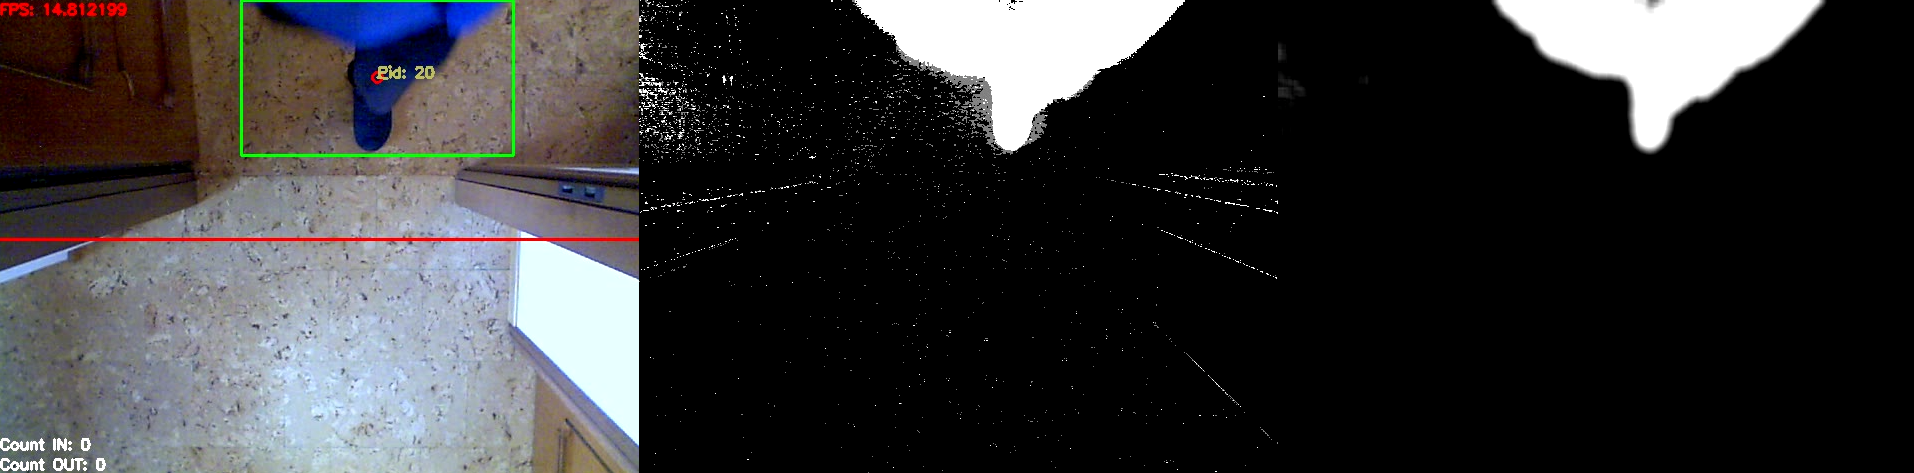
\includegraphics[width=\linewidth]{PCNTest1.png}
  \caption{Risultato test PCN a sottrazione del background: frame 1.}
  \label{fig:PCNTest1}
\end{figure}

\begin{figure}[h!]
  \centering
  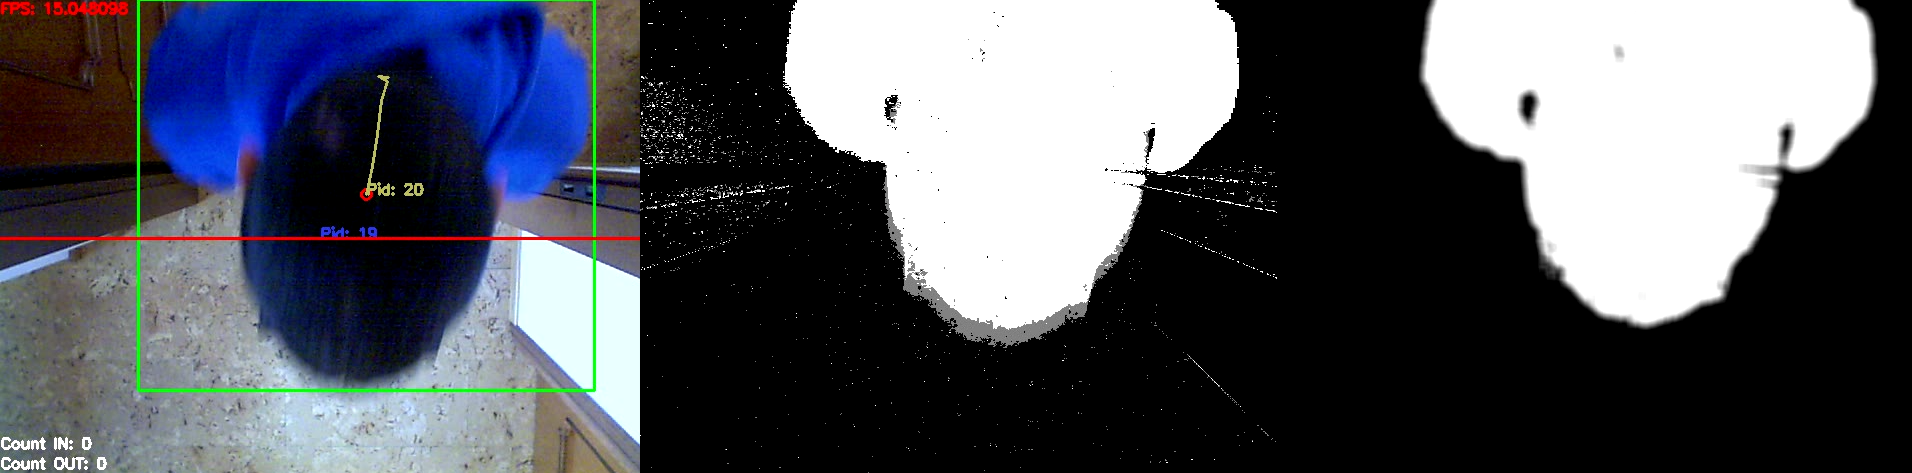
\includegraphics[width=\linewidth]{PCNTest2.png}
  \caption{Risultato test PCN a sottrazione del background: frame 2.}
  \label{fig:PCNTest2}
\end{figure}

\begin{figure}[h!]
  \centering
  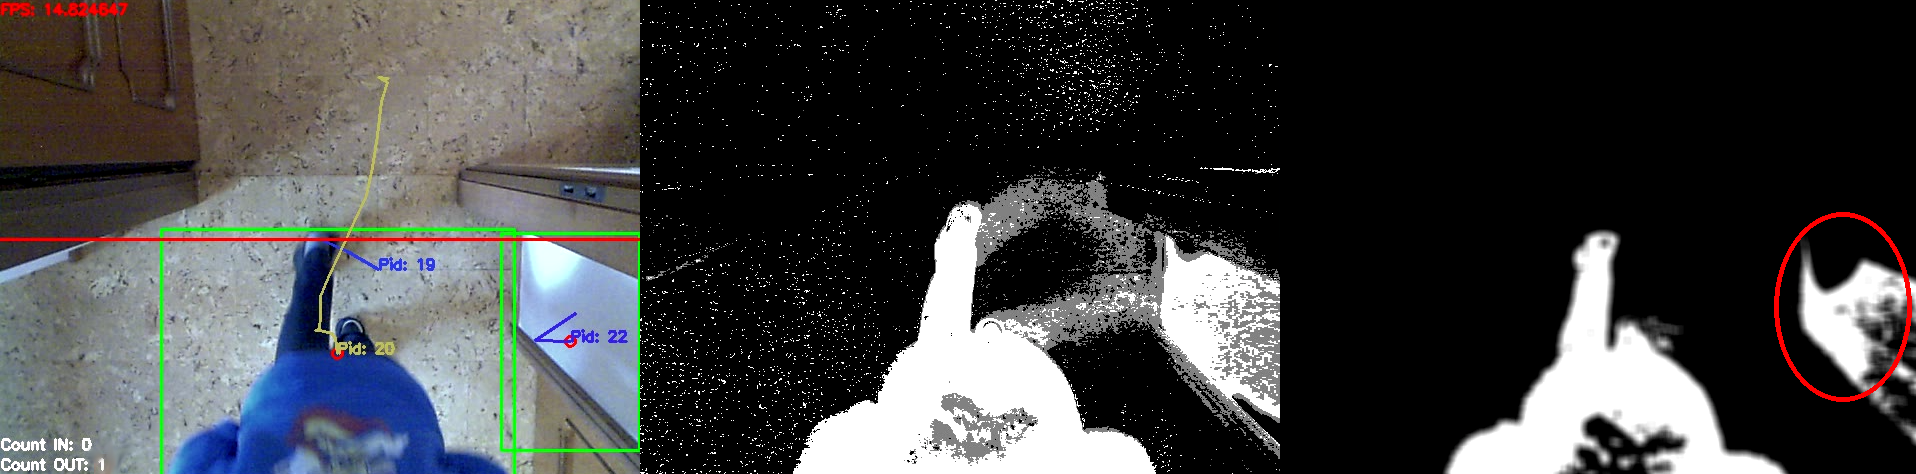
\includegraphics[width=\linewidth]{PCNTest3.png}
  \caption{Risultato test PCN a sottrazione del background: frame 3.}
  \label{fig:PCNTest3}
\end{figure}

%% Interruzione di pagina
\newpage

In figura \ref{fig:PCNTest3} \`e importante notare l'effetto di riduzione del rumore ed eliminazione dell'ombra ottenuti. Nonostrante ci\`o l'ombra proiettata lateralmente sul muro viene rilevata erroneamente come oggetto in movimento. Essa viene quindi tracciata dal programma e rilevata come passeggero.

Inoltre, al centro del fotogramma, \`e possibile notare un ulteriore falso tracciamento dovuto ad un picco di rumore registrato dalla telecamera.

\begin{figure}[h!]
  \centering
  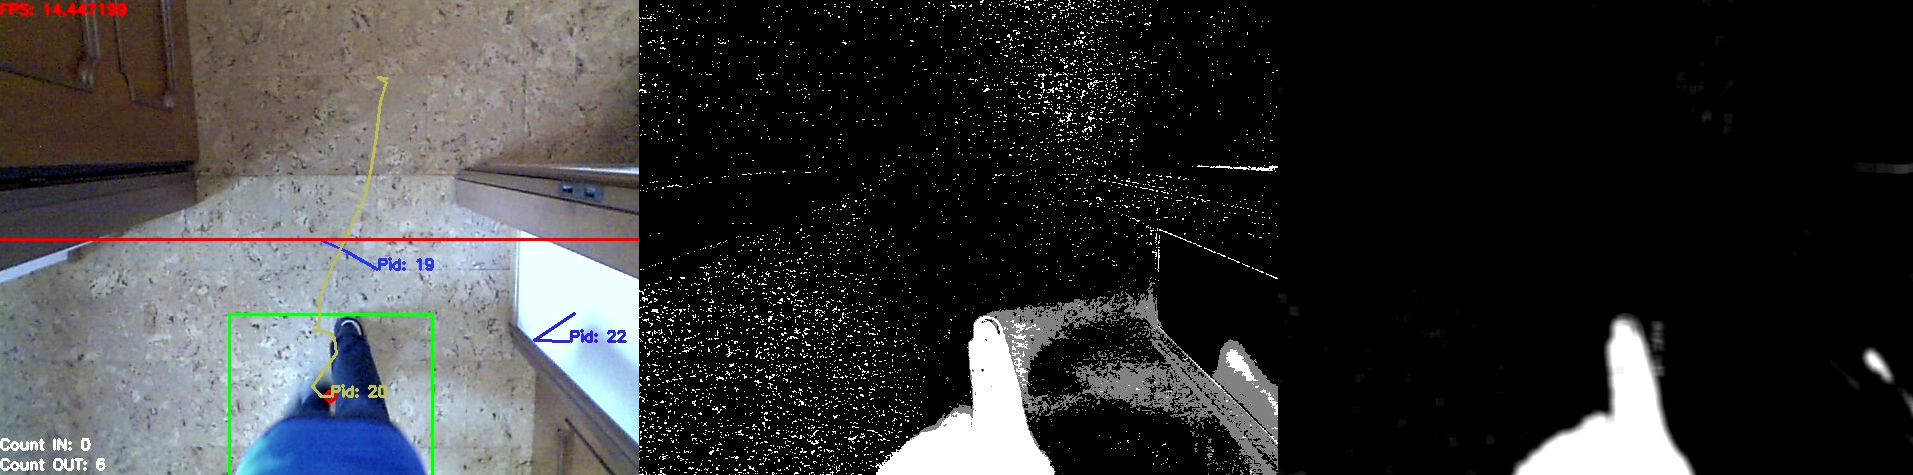
\includegraphics[width=\linewidth]{PCNTest4.png}
  \caption{Risultato test PCN a sottrazione del background: frame 4.}
  \label{fig:PCNTest4}
\end{figure}

In figura \ref{fig:PCNTest4} \`e nuovamente possibile notare l'effetto di riduzione del rumore molto elevato in questo frame. Si noti come in questo caso l'ombra proiettata sul muro laterale sia correttamente rilevata come ombra e quindi eliminata dalle operazioni di riduzione del rumore. Nel frame a colori \`e possibile notare come l'ombra sul muro abbia lasciato una scia di tracciamento, ci\`o \`e dovuto al fatto che, pur essendo sparita dal raggio visivo, il suo parametro \verb|age| non ha ancora raggiunto il valore massimo, e quindi non \`e ancora stata eliminata dalla memoria.

%% Interruzione di pagina
\newpage

%TODO: Inserire grafico per vedere meglio le performance
\subsubsection{Performance}
Per la misura dei tempi di esecuzione si \`e fatto uso della libreria standard \verb|chrono| di C++. I test sono stati effettuati usando due telecamere di pari risoluzione ma con diverso framerate su due diversi dispositivi: il ReliaGate 20-25 ed una macchina Linux ad alte prestazioni. I tempi sono stati mediati sul numero di cicli effettuati, cio\`e pari al numero di frame catturati dalla telecamera.

Nel seguito sono riportati i risultati relativi alle performance dell'applicazione utilizzando la webcam descritta nel paragrafo \ref{HardwarePCN}: 

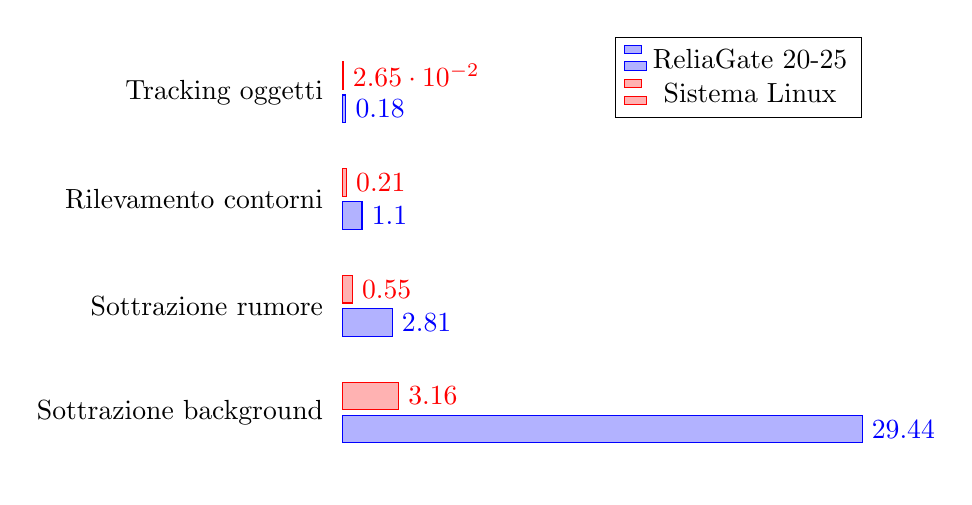
\begin{tikzpicture}
\begin{axis}[
  xbar,
  y axis line style = { opacity = 0 },
  axis x line       = none,
  tickwidth         = 0pt,
  enlarge y limits  = 0.2,
  enlarge x limits  = 0.02,
  symbolic y coords = {Sottrazione background, Sottrazione rumore, Rilevamento contorni, Tracking oggetti},
  nodes near coords,
]
% ReliaGate 20-25
\addplot 
    coordinates {(29.4414,Sottrazione background) (2.80683,Sottrazione rumore) (1.09507,Rilevamento contorni) 
                    (0.178409,Tracking oggetti)};
% Sistema Linux
\addplot 
    coordinates {(3.16497,Sottrazione background) (0.546563,Sottrazione rumore) (0.211879,Rilevamento contorni) 
                    (0.026478,Tracking oggetti)};
\legend{ReliaGate 20-25, Sistema Linux}
\end{axis}
\end{tikzpicture}

\begin{table}[h!]
    \centering
	\begin{tabular}{|l|c|c|}
	\hline
    & ReliaGate 20-25 & Sistema Linux \\ \hline
    Tempo di esecuzione del loop principale & 41.254 ms & 31.1649 ms \\ \hline
    Algoritmo sottrazione del background & 29.4414 ms & 3.16497 ms \\ \hline
    Sottrazione del rumore & 2.80683 ms & 0.546563 ms \\ \hline
    Algoritmo rilevamento contorni & 1.09507 ms & 0.211879 ms \\ \hline
    Rilevamento e tracking degli oggetti & 0.178409 ms & 0.026478 ms \\ \hline
    Frame Rate & 20.1 FPS & 30 FPS \\ \hline
	\end{tabular}
    \caption{Risultati Passenger Counter a sottrazione del background con webcam 30 FPS}
\end{table}

Si noti che il tempo di esecuzione del loop principale considera anche il tempo speso ad attendere i frame dalla telecamera.

Nel seguito sono riportati i risultati relativi alle performance dell'applicazione utilizzando una webcam capace di fornire uno stream a 60 FPS ma con la stessa risoluzione della precedente:

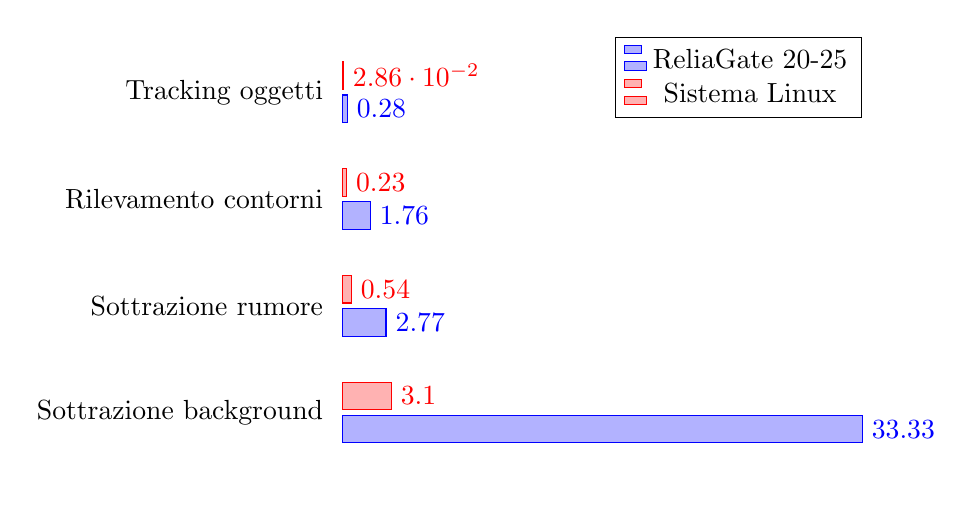
\begin{tikzpicture}
\begin{axis}[
  xbar,
  y axis line style = { opacity = 0 },
  axis x line       = none,
  tickwidth         = 0pt,
  enlarge y limits  = 0.2,
  enlarge x limits  = 0.02,
  symbolic y coords = {Sottrazione background, Sottrazione rumore, Rilevamento contorni, Tracking oggetti},
  nodes near coords,
]
% ReliaGate 20-25
\addplot 
    coordinates {(33.3335,Sottrazione background) (2.7739,Sottrazione rumore) (1.75694,Rilevamento contorni) 
                    (0.279599,Tracking oggetti)};
% Sistema Linux
\addplot 
    coordinates {(3.10198,Sottrazione background) (0.538276,Sottrazione rumore) (0.233947,Rilevamento contorni) 
                    (0.028581,Tracking oggetti)};
\legend{ReliaGate 20-25, Sistema Linux}
\end{axis}
\end{tikzpicture}

%% Interruzione di pagina
\newpage

\begin{table}[h!]
    \centering
	\begin{tabular}{|l|c|c|}
	\hline
    & ReliaGate 20-25 & Sistema Linux \\ \hline
    Tempo di esecuzione del loop principale & 46.7684 ms & 15.7044 ms \\ \hline
    Algoritmo sottrazione del background & 33.3335 ms & 3.10198 ms \\ \hline
    Sottrazione del rumore & 2.7739 ms & 0.538276 ms \\ \hline
    Algoritmo rilevamento contorni & 1.75694 ms & 0.233947 ms \\ \hline
    Rilevamento e tracking degli oggetti & 0.279599 ms & 0.028581 ms \\ \hline
    Frame Rate & 20.5 FPS & 60 FPS \\ \hline
	\end{tabular}
    \caption{Risultati Passenger Counter a sottrazione del background con webcam 30 FPS}
\end{table}

Come evidenziato dai dati riportati nelle tabelle la funzione pi\`u onerosa del punto di vista computazionale \`e quella che applica l'algoritmo di sottrazione del background. Inoltre si pu\`o notare come nel caso del 20-25, la computazione occupa talmente tanto tempo da compromettere la stabilit\`a del framerate. Nominalmente il flusso video dovrebbe essere stabile sui 30 FPS ma per il 20-25 si ferma a circa 20 frame al secondo. L'utilizzo di una telecamera con risoluzione pi\`u elevata comprometterebbe ulteriormente le performance a causa del maggior numero di pixel sul quale effettuare la computazone.

Infine \`e opportuno notare che, la durata del loop principale nel caso della telecamera a 30 FPS, \`e simile sui due sistemi poich\`e quello pi\`u performante impiega la maggior parte del tempo ad aspettare i frame. La funzione \verb|cap.read()| \`e infatti bloccante. Questo non si verifica invece nel caso della telecamera a 60 FPS poich\`e fornisce frame pi\`u velocemente.

%% Interruzione di pagina
\newpage

\subsection{Problemi}
I problemi principali rilevati in questa implementazione del Passenger Counter sono i seguenti:
\begin{enumerate}
\item \textbf{Imprecisione}: Le immagini risultati dalla sottrazione del background tendono ad essere molto rumorose, nonostante il post-processing applicato. Il conteggio ne risulta influenzato negativamente.
\item \textbf{Tracciamenti indesiderati}: Come visto nel paragrafo precedente, nonostante l'algoritmo riesca a rilevare la maggior parte delle ombre come tali, spesso le ombre vengono tracciate erroneamente. Ci\`o comporta errori nel conteggio.
\item \textbf{Performance}: L'algoritmo di sottrazione del background, come riportato nel paragrafo precedente, \`e piuttosto oneroso dal punto di vista computazionale. Ci\`o ne limita le possibili applicazioni: non \`e possibile utilizzare telecamere con risoluzione elevata e bisogna limitare il numero di telecamere utilizzate contemporaneamente.
\item \textbf{Tecnologia}: Il problema pi\`u grave \`e senz'altro determinato dalla tecnologia utilizzata. La tecnica della background subtraction si basa sulla costruzione di un modello di background costruito a partire dalle immagini ricavate dalla telecamera. Un ambiente come quello di un mezzo pubblico \`e troppo dinamico perch\`e l'algoritmo possa costruire un modello di background affidabile: le condizioni di luce cambiano con troppa frequenza.
\end{enumerate}

Per questo motivo si \`e passati ad una seconda implementazione sfruttando una tecnologia esente da queste problematiche: il Passenger Counter con telecamere RealSense.

%% Interruzione di pagina
\newpage

% TODO: Aggiornare questo preambolo in base a cosa andrai a scrivere nelle sezioni seguenti.
\section{Passenger Counter con telecamere RealSense}
In questa sezione tratteremo la versione del contatore di passeggeri che utilizza le telecamere RealSense. Inizialmente descriveremo la struttura del codice, gli algoritmi utilizzati ed il suo funzionamento. Infine parleremo dei risultati ottenuti da questa implementazione e le problematiche principali.

Poich\`e questa versione \`e basata interamente sulla versione del contatore di passeggeri a sottrazione del background, per evitare ripetizioni, ci concentreremo sulle differenze tra le due versioni.

\subsection{Struttura del codice}
In figura \ref{fig:RSPCNUML} \`e riportato il diagramma UML del Passenger Counter con telecamere RealSense. La struttura rimane molto simile a quella utilizzata per il contatore a sottrazione del background:

\begin{enumerate}
\item \textbf{Passenger}: \`e la stessa classe usata nella versione precedente del programma.
\item \textbf{RSPCN}: \`e la classe che implementa il contatore di passeggeri. Questa fa uso della libreria librealsense di cui si \`e discusso nel paragrafo \ref{librealsense}.
\item \textbf{main}: implementa l'interfaccia utente per gestire i settaggi run-time delle telecamere e del contatore. Si noti inoltre che rileva automaticamente il numero di telecamere collegate e instanzia un contatore per ogniuna di esse.
\end{enumerate}

%% Interruzione di pagina
\newpage

\begin{figure}[h!]
  \centering
  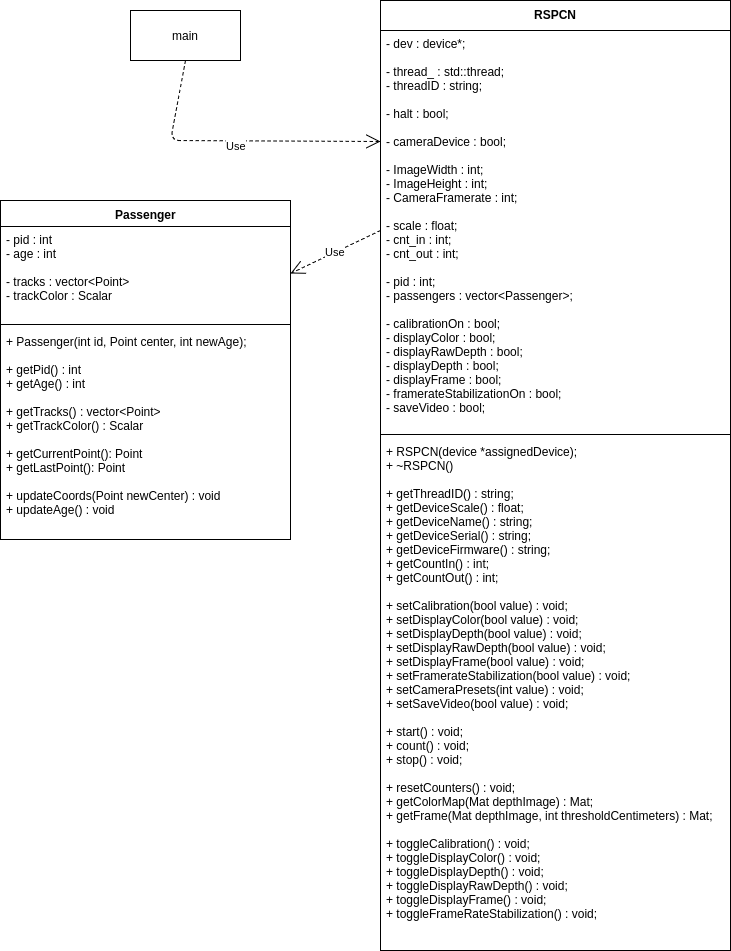
\includegraphics[width=\textwidth]{RSPCNUML.png}
  \caption{Diagramma UML del Passenger Counter con telecamere RealSense}
  \label{fig:RSPCNUML}
\end{figure}

%% Interruzione di pagina
\newpage

\subsection{Classe RSPCN}
Questa classe ha gli stessi obiettivi della classe PCN nel caso del Passenger Counter a sottrazione del background, con qualche aggiunta. Essa deve infatti:

\begin{itemize}
\item Interfacciarsi con le telecamere RealSense per mezzo della libreria librealsense in modo da poterne controllare i settaggi in tempo reale e ricavare i dati di profondit\`a.
\item Convertire i dati ottenuti dalle telecamere RealSense in qualcosa di utilizzabile dall'algoritmo.
\end{itemize}

Qui di seguito \`e riportato l'header della classe RSPCN:

\begin{lstlisting}[language=C++, caption=RSPCN.h]
class RSPCN {

public:
  // Constructor
  RSPCN(device *assignedDevice);
  ~RSPCN() { thread_.join(); }

  // Selectors
  string getThreadID(){return threadID;};
  float getDeviceScale(){return scale;};
  string getDeviceName(){return dev->get_name();};
  string getDeviceSerial(){return dev->get_serial();};
  string getDeviceFirmware(){return dev->get_firmware_version();};

  int getCountIn(){return cnt_in;};
  int getCountOut(){return cnt_out;};

  // Setters
  void setCalibration(bool value) {calibrationOn = value; return;};
  void setDisplayColor(bool value) {displayColor = value; return;};
  void setDisplayDepth(bool value) {displayDepth = value; return;};
  void setDisplayRawDepth(bool value) {displayRawDepth = value; return;};
  void setDisplayFrame(bool value) {displayFrame = value; return;};
  void setFramerateStabilization(bool value) {framerateStabilizationOn = value; return;};
  void setCameraPresets(int value);
  void setSaveVideo(bool value) {saveVideo = value; return;};

  // Methods
  void start();
  void count();
  void stop(){halt = true;};

  void resetCounters(){cnt_in = 0; cnt_out = 0; return;};

  Mat getColorMap(Mat depthImage);
  Mat getFrame(Mat depthImage, int thresholdCentimeters);
  
  void toggleCalibration();
  void toggleDisplayColor();
  void toggleDisplayDepth();
  void toggleDisplayRawDepth();
  void toggleDisplayFrame();
  void toggleFrameRateStabilization(){framerateStabilizationOn = !framerateStabilizationOn; return;};

private:
  device * dev;

  std::thread thread_;
  string threadID;

  bool halt = false;

  // Camera type
  bool cameraDevice;

  // Camera options
  int ImageWidth;
  int ImageHeight;
  int CameraFramerate;

  // Camera scale
  float scale;

  // Passenger counters
  int cnt_in  = 0;
  int cnt_out = 0;

  // Passengers tracker
  int pid = 0;
  vector<Passenger> passengers;

  // Options
  bool calibrationOn = false;
  bool displayColor = false;
  bool displayRawDepth = false;
  bool displayDepth = false;
  bool displayFrame = false;
  bool framerateStabilizationOn = true;
  bool saveVideo = false;
};
\end{lstlisting}

%% Interruzione di pagina
\newpage

I punti rilevanti dell'header sono i seguenti:

\begin{itemize}
\item La funzione \verb|count()| anche in questo caso rappresenta il cuore del Passenger Counter e verr\`a analizzata separatamente.
\item La variabile \verb|dev| di tipo \verb|device| \`e la telecamera dalla quale il contatore raccoglie i dati. Questo tipo \`e definito nella libreria delle telecamere RealSense ed \`e usato per andare a raccogliere i frame in uscita dalla telecamera, nonch\`e altri dati utili per il funzionamento del programma.
\item La variabile \verb|cameraDevice| si \`e resa necessaria per poter distinguere le due telecamere usate durante lo sviluppo del progetto poich\`e necessitano di settaggi diversi per il loro funzionamento.
\item I metodi \verb|getColorMap()| e \verb|getFrame()| sono le funzioni che convertono i frame forniti dalle telecamere RealSense in qualcosa di utilizzabile dal nostro algoritmo. Nel seguito vedremo in dettaglio cosa fanno.
\end{itemize}

%% Interruzione di pagina
\newpage

\subsection{Metodo getColorMap()}
Questo metodo \`e stato molto utile in fase di sviluppo poich\`e fornisce una rappresentazione dei dati in uscita dalla telecamera molto intuitiva. Non ha un ruolo funzionale all'interno dell'algoritmo ma facilita la comprensione di quanto accade al suo interno quindi \`e opportuno spiegarne il funzionamento.

\begin{lstlisting}[language=C++, caption=RSPCN.cpp metodo getColorMap()]
Mat RSPCN::getColorMap(Mat depthImage) {
    Mat depthColorMap;

    double min;
    double max;
    Point tmpMinLoc;
    Point tmpMaxLoc;

    int nearestVal;
    Point nearestLoc;

    int farthestVal;
    Point farthestLoc;

    // Saving farthest point
    minMaxLoc(depthImage, &min, &max, &tmpMinLoc, &tmpMaxLoc);
    farthestVal = max;
    farthestLoc = tmpMaxLoc;

    // If pixelValue == 0 set it to 65535( = 2^16 - 1)
    depthImage.setTo(65535, depthImage == NODATA);

    // Saving nearest point
    minMaxLoc(depthImage, &min, &max, &tmpMinLoc, &tmpMaxLoc);
    nearestVal = min;
    nearestLoc = tmpMinLoc;

    // Converts CV_16U to CV_8U using a scale factor of 255.0/ 65535
    depthImage.convertTo(depthImage, CV_8UC1, 255.0 / 65535);

    // Current situation: Nearest object => Black, Farthest object => White
    // We want to have  : Nearest object => White, Farthest object => Black
    depthImage = cv::Scalar::all(255) - depthImage;

    // Color map: Nearest object => Red, Farthest object => Blue
    equalizeHist( depthImage, depthImage );
    applyColorMap(depthImage, depthColorMap, COLORMAP_JET);

    // Highlight nearest and farthest pixel
    circle( depthColorMap, nearestLoc, 5, WHITE, 2, 8, 0 );
    putText(depthColorMap, "Nearest: " + to_string(nearestVal*scale) + " m", Point(0, depthColorMap.rows - 30), FONT_HERSHEY_SIMPLEX, 0.5, WHITE, 2);

    circle( depthColorMap, farthestLoc, 5, WHITE, 2, 8, 0 );
    putText(depthColorMap, "Farthest: " + to_string(farthestVal*scale) + " m", Point(0, depthColorMap.rows - 10), FONT_HERSHEY_SIMPLEX, 0.5, WHITE, 2);

    return depthColorMap;
}
\end{lstlisting}

Come si \`e detto nel paragrafo \ref{librealsense} l'output delle telecamere RealSense \`e dato da delle immagini in scala di grigi i cui pixel hanno formato 16 bit privi di segno, i quali rappresentano la distanza del pixel dalla telecamera. Il valore 0 significa che non si \`e potuti ricavare dati sulla distanza. Questo \`e il formato dell'immagine che ci aspettiamo in ingresso alla funzione e in figura \ref{fig:rawDepthImage} \`e riportato il risultato di un plot per mezzo di OpenCV di questo formato di immagini.

\begin{figure}[h!]
\begin{minipage}[b]{8.5cm}
  \centering
  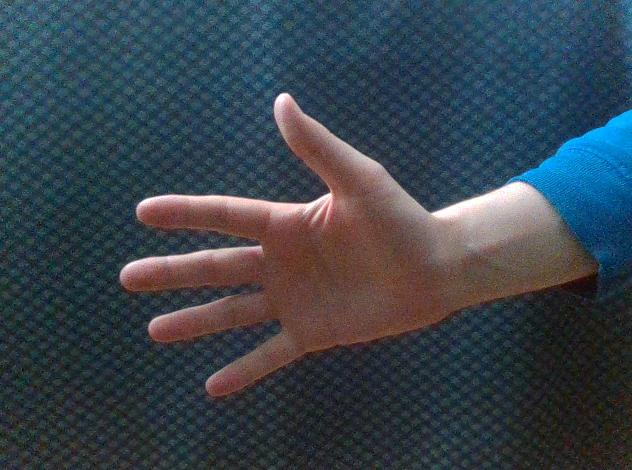
\includegraphics[width=8cm]{rawDepthImageC.png}
  \caption{Output Intel RealSense SR300 colori.}
  \label{fig:colorSR300}
\end{minipage}
\ \hspace{2mm} \hspace{3mm} \
\begin{minipage}[b]{8.5cm}
 \centering
  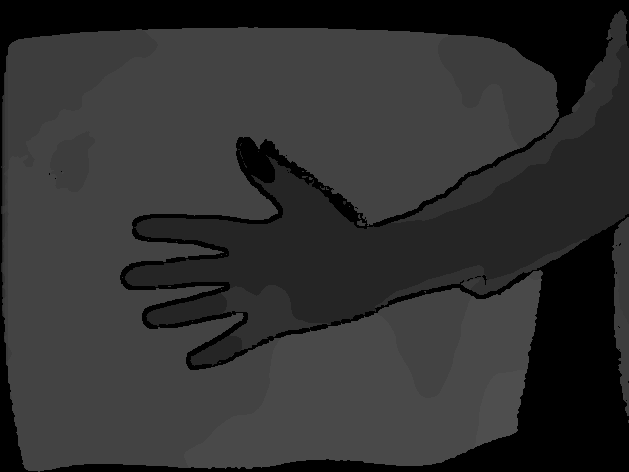
\includegraphics[width=8cm]{rawDepthImageD.png}
  \caption{Output Intel RealSense SR300 grezzo.}
  \label{fig:rawDepthImage}
\end{minipage}
\end{figure}

Si noti che la leggera discrepanza tra le due immagini \`e dovuta al fatto che il sensore a infrarossi e quello per le immagini a colori si trovano in posizioni diverse. Inoltre il sensore a infrarossi ha un FOV pi\`u elevato.

\subsubsection{Funzionamento getColorMap()}
Il primo step \`e portare il valore dei pixel per i quali non \`e stato possibile ricavare il dato di distanza alla massima distanza rappresentabile. Quindi portiamo tutti i pixel nulli a 65535. Questo \`e implementato dalla funzione \verb|setTo()|.

Quindi convertiamo l'immagine da 16 bit a 8 bit usando un fattore di scala. Si noti che questa conversione \`e con perdita.

Otteniamo il risultato in figura \ref{fig:getColorMapStep1}.

%% Interruzione di pagina
\newpage

\begin{figure}[h!]
\begin{minipage}[b]{8.5cm}
  \centering
  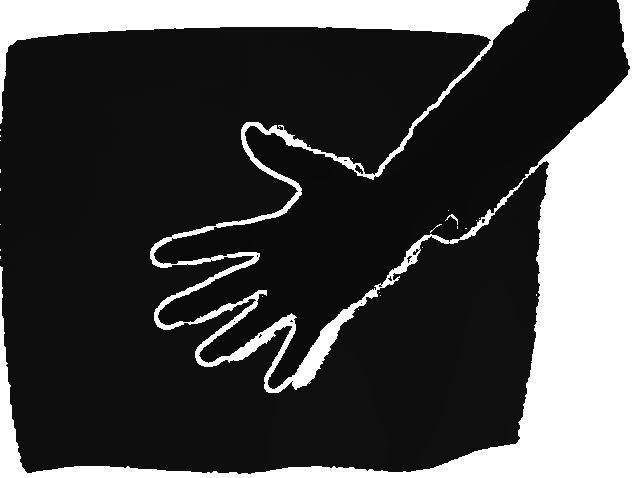
\includegraphics[width=8cm]{getColorMapStep1.png}
  \caption{getColorMap step 1}
  \label{fig:getColorMapStep1}
\end{minipage}
\ \hspace{2mm} \hspace{3mm} \
\begin{minipage}[b]{8.5cm}
 \centering
  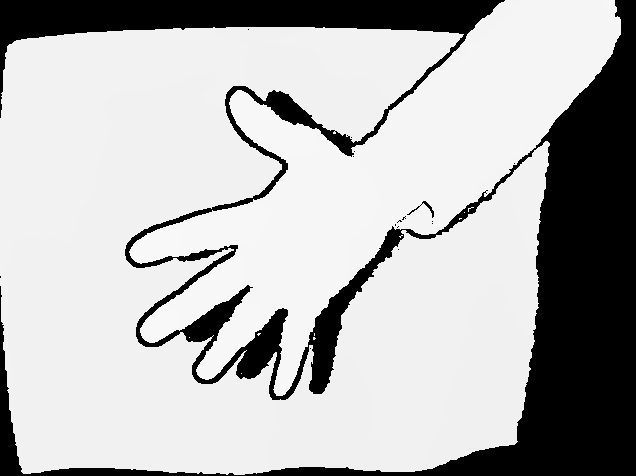
\includegraphics[width=8cm]{getColorMapStep2.png}
  \caption{getColorMap step 2}
  \label{fig:getColorMapStep2}
\end{minipage}
\end{figure}

A questo punto vogliamo rappresentare i pixel pi\`u vicini con colori pi\`u chiari e i pixel pi\`u lontani con colori pi\`u scuri. Per ottenere ci\`o \`e sufficiente sottrarre l'immagine ad un matrice delle stesse dimensioni in cui tutti i pixel sono bianchi. Otteniamo l'immagine in figura \ref{fig:getColorMapStep2}:

Quindi passiamo l'immagine cos\`\i\ ottenuta alla funzione \verb|equalizeHist()| la quale aumenta il contrasto dell'immagine che le viene passata come argomento. In questo modo i colori che rappresentano la distanza nell'immagine risultano pi\`u evidenti. Poich\'e questa funzione accetta in ingresso solamente immagini a 8 bit si \`e resa necessaria la conversione con perdita.

In figura \ref{fig:getColorMapStep3} il risultato dell'applicazione della funzione.

\begin{figure}[h!]
\begin{minipage}[b]{8.5cm}
  \centering
  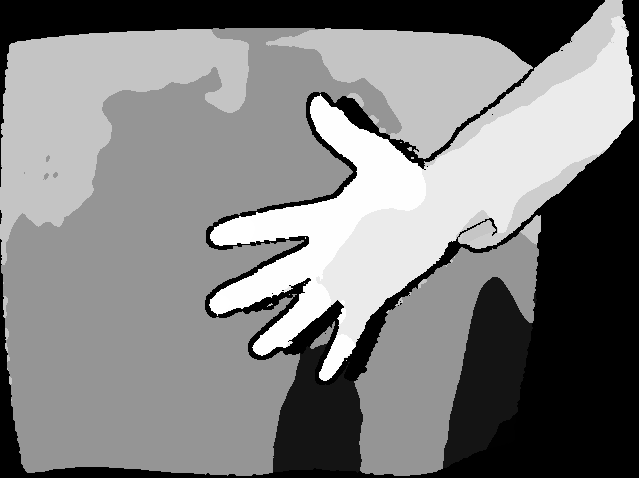
\includegraphics[width=8cm]{getColorMapStep3.png}
  \caption{getColorMap step 3}
  \label{fig:getColorMapStep3}
\end{minipage}
\ \hspace{2mm} \hspace{3mm} \
\begin{minipage}[b]{8.5cm}
 \centering
  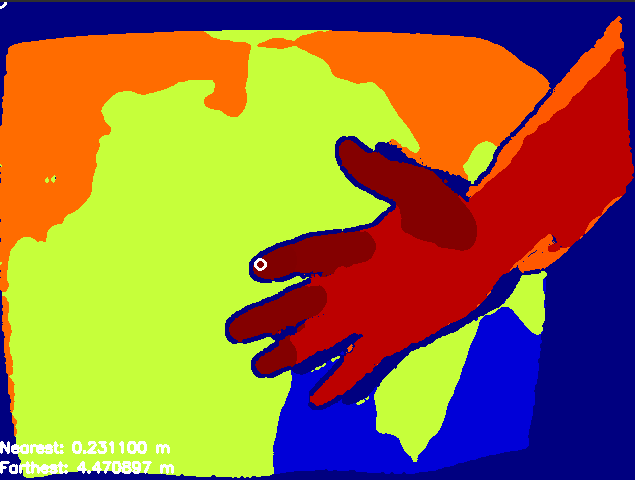
\includegraphics[width=8cm]{getColorMapStep4.png}
  \caption{getColorMap step 4}
  \label{fig:getColorMapStep4}
\end{minipage}
\end{figure}

Infine viene applicata la funzione \verb|applyColorMap()| la quale va semplicemente a ricolorare l'immagine in scala di grigi per avere una migliore percezione delle informazioni fornite dalle telecamere RealSense.

Si noti infine che durante questa elaborazione sono stati conservati i dati del pixel pi\`u lontano e pi\`u vicino e convertiti in distanza. Ci\`o ha aiutato molto durante lo sviluppo del progetto per poter calibrare al meglio il contatore.

%% Interruzione di pagina
\newpage

\subsection{Metodo getFrame()}
Questo metodo \`e alla base del funzionamento di questa versione del Passenger Counter. Esso va a recuperare i dati forniti dalle telecamere RealSense e li converte in un formato che pu\`o essere dato in pasto allo stesso algoritmo usato a valle della sottrazione del background nella precedente versione del contatore.

Qui di seguito \`e riportato il codice della funzione:

\begin{lstlisting}[language=C++, caption=RSPCN.cpp metodo getFrame()]
Mat RSPCN::getFrame(Mat depthImage, int thresholdCentimeters) {
    Mat frame;

    // If depthImage(x,y) == NODATA, set it to 65535
    depthImage.setTo(65535, depthImage == NODATA);

    // Threshold only accepts CV_8U or CV_32F types
    depthImage.convertTo(depthImage, CV_32FC1);

    // Converting threshold from cm to pixel value
    int threshPixel = thresholdCentimeters / (100*scale);

    // Applying threshold
    threshold(depthImage, depthImage, threshPixel, 65535, THRESH_BINARY);

    // Convert to CV_8U (lossy conversion)
    depthImage.convertTo(depthImage, CV_8UC1, 255.0 / 65535);

    // Invert b&w: white = foreground, black= background.
    frame = cv::Scalar::all(255) - depthImage;

    return frame;
}
\end{lstlisting}

In ingresso abbiamo sempre il formato immagine illustrato in figura \ref{fig:rawDepthImage} e la soglia espressa in centimetri da applicare all'immagine in ingresso.

Come nel caso precedente partiamo applicando la funzione \verb|setTo()| per imporre tutti i pixel nulli a 65535. Quindi convertiamo l'immagine da 16 bit privi di segno a 32 bit floating point. Questo passaggio  \`e necessario per poter dare in pasto l'immagine alla funzione \verb|threshold()|, la quale accetta solamente immagini nel formato 8 bit privi di segno o 32 bit floating point. Il risultato di questo passaggio \`e visibile in figura \ref{fig:getFrameStep1}.

Passiamo quindi ad applicare la soglia sull'immagine. Siccome i valori dei pixel rappresentano una distanza possiamo eliminare tutto ci\`o che si trova oltre una certa distanza dalla telecamera per mezzo della funzione \verb|threshold()|. Anzitutto \`e necessario convertire la soglia da cm al valore numerico applicabile sui pixel, quindi si passa all'applicazione della soglia vera e propria.

\verb|scale| \`e la scala alla quale \`e impostata la telecamera e viene ricavata interrogandola per mezzo della libreria librealsense. Va moltiplicata per un fattore cento in quanto l'unit\`a di misura con la quale viene fornita sono i metri e noi abbiamo una soglia espressa in centimetri.

%% Interruzione di pagina
\newpage

La soglia va quindi ad applicare la seguente operazione:

\begin{equation}
dstPixel(x,y) = \begin{cases} 65535, & \mbox{se } srcPixel(x,y) > threshPixel \\ 0, & \mbox{altrimenti } \end{cases}
\end{equation}

In sostanza vengono eliminati dall'immagine tutti gli oggetti che si trovano ad una distanza dalla telecamera maggiore della soglia impostata. Si noti che a questo punto si sono perse tutte le informazioni di distanza date dai valori dei pixel. 

Ora \`e possibile convertire l'immagine al formato 8 bit privi di segno applicando un semplice fattore di scala per mezzo della funzione \verb|convertTo()|. In figura \ref{fig:getFrameStep2} \`e riportato il risultato dell'operazione di soglia e conversione nel formato 8 bit. Si pu\`o notare come lo sfondo sia stato completamente rimosso. 

\begin{figure}[h!]
\begin{minipage}[b]{8.5cm}
  \centering
  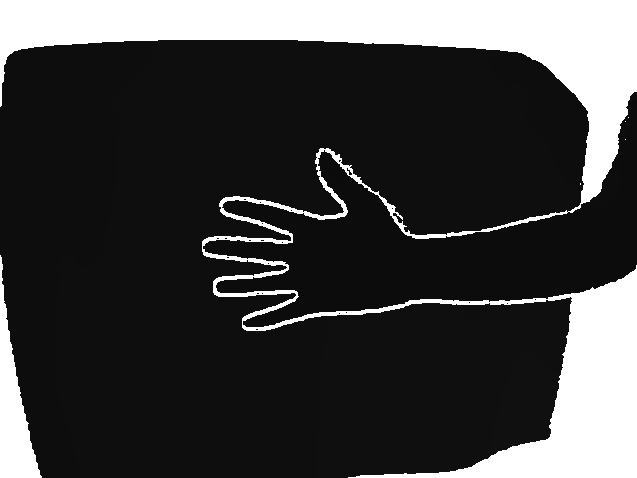
\includegraphics[width=8cm]{getFrameStep1.png}
  \caption{getFrame step 1}
  \label{fig:getFrameStep1}
\end{minipage}
\ \hspace{2mm} \hspace{3mm} \
\begin{minipage}[b]{8.5cm}
 \centering
  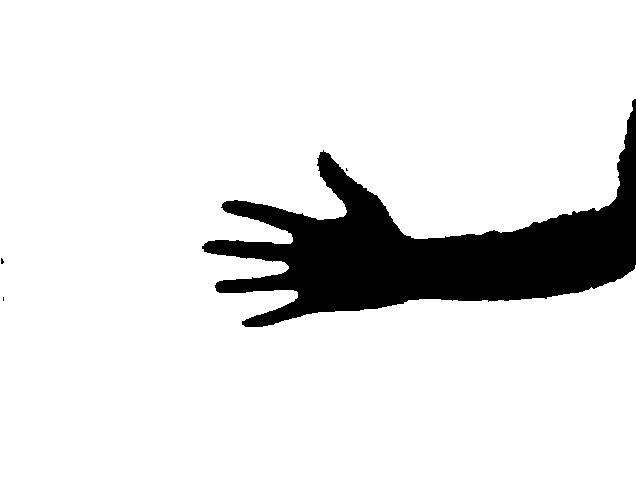
\includegraphics[width=8cm]{getFrameStep2.png}
  \caption{getFrame step 2}
  \label{fig:getFrameStep2}
\end{minipage}
\end{figure}

Infine, poich\'e vogliamo avere che gli oggetti in primo piano siano bianchi e gli oggetti dello sfondo neri, non ci resta che sottrarre l'immagine ad un matrice delle stesse dimensioni in cui tutti i pixel sono bianchi. Il risultato \`e riportato in figura \ref{fig:getFrameStep3}.

\begin{figure}[h!]
  \centering
  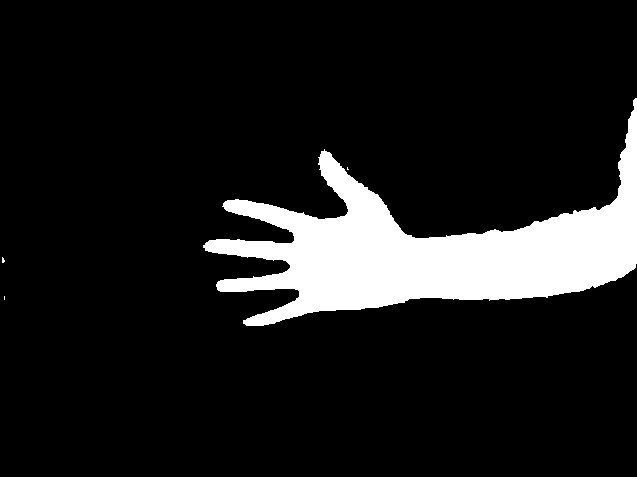
\includegraphics[width=9cm]{getFrameStep3.png}
  \caption{getFrame step 3}
  \label{fig:getFrameStep3}
\end{figure}

%% Interruzione di pagina
\newpage

\subsection{Analisi del kernel del programma: funzione count()}
La funzione \verb|count()|, anche per questa versione del contatore, \`e il cuore del programma. Il codice \`e suddivisibile ancora una volta in tre sezioni:

\begin{enumerate}
\item Estrazione degli oggetti in primo piano.
\item Rilevamento e tracking degli oggetti di nostro interesse.
\item Conteggio degli attraversamenti.
\end{enumerate}

\`E stato possibile riutilizzare il codice della versione del contatore a sottrazione del background per le ultime due sezioni. Discorso a parte va fatto per il primo punto.

\subsubsection{Estrazione degli oggetti in primo piano}

\begin{lstlisting}[language=C++, caption=RSPCN.cpp metodo count()]
void RSPCN::count()
{
    // Streams
    Mat frame;
    Mat rawDepth;
    Mat morphTrans;
    Mat depthColorMap;

    // Contours variables
    vector<vector<Point> > contours;
    vector<Vec4i> hierarchy;

    // Calibration
    int thresholdCentimeters = MAX_RANGE_CM;
    int blur_ksize = BLUR_KSIZE;
    int areaMin = AREA_MIN;
    int xNear = X_NEAR;
    int yNear = Y_NEAR;
    int maxPassengerAge = MAX_PASSENGER_AGE;

    // Execution time
    duration<double> loopTime;
    bool firstLoop = true;

    // Start streaming
    dev->start();

    while(!halt)
    {
        // Synchronization
        if( dev->is_streaming( ) )
        {
            if(framerateStabilizationOn)
                dev->wait_for_frames( );
            else
                dev->poll_for_frames(); // Non blocking option
        }

        // Get frame data
        Mat color(Size(ImageWidth, ImageHeight), CV_8UC3, (void*)dev->get_frame_data(rs::stream::color), Mat::AUTO_STEP);
        Mat depth(Size(ImageWidth, ImageHeight), CV_16U , (void*)dev->get_frame_data(rs::stream::depth), Mat::AUTO_STEP);

        // -- CONVERTING DEPTH IMAGE AND THRESHOLDING
        frame = getFrame(depth, thresholdCentimeters);

        // -- DENOISING
        blur(frame, morphTrans, Size(blur_ksize,blur_ksize));

        // --FINDING CONTOURS
        findContours(morphTrans, contours, hierarchy, RETR_EXTERNAL, CHAIN_APPROX_NONE);

        // For every detected object
        for(unsigned int idx = 0; idx < contours.size(); idx++)
        {
            ...
        }
        ...
    }
    ...
}
\end{lstlisting}

Il procedimento \`e pressoch\`e identico alla versione precedente:

\begin{enumerate}
\item Vengono catturati i frame dalla telecamera RealSense utilizzando la funzione \verb|get_frame_data()| resa disponibile dalla libreria RealSense.
\item Questi frame vengono convertiti in un formato utilizzabile dalla funzione \verb|findContours()| di OpenCV grazie alla funzione \verb|getFrame()| di cui si \`e parlato nel paragrafo precedente.
\item Si effettua una veloce operazione di riduzione del rumore.
\end{enumerate}

Da questo punto in poi il codice rimane identico alla versione a sottrazione del background trattata nella sezione \ref{kernelPCN} a pagina \pageref{kernelPCN}.

%% Interruzione di pagina
\newpage

Come nel caso precedente si \`e deciso di plottare a schermo tutte le informazioni utili a semplificare la comprensione del funzionamento del programma e al debugging. Un esempio della schermata tipica durante il funzionamento del contatore in fase sperimentale \`e riportato in figura \ref{fig:RSPCN}.

\begin{figure}[h!]
  \centering
  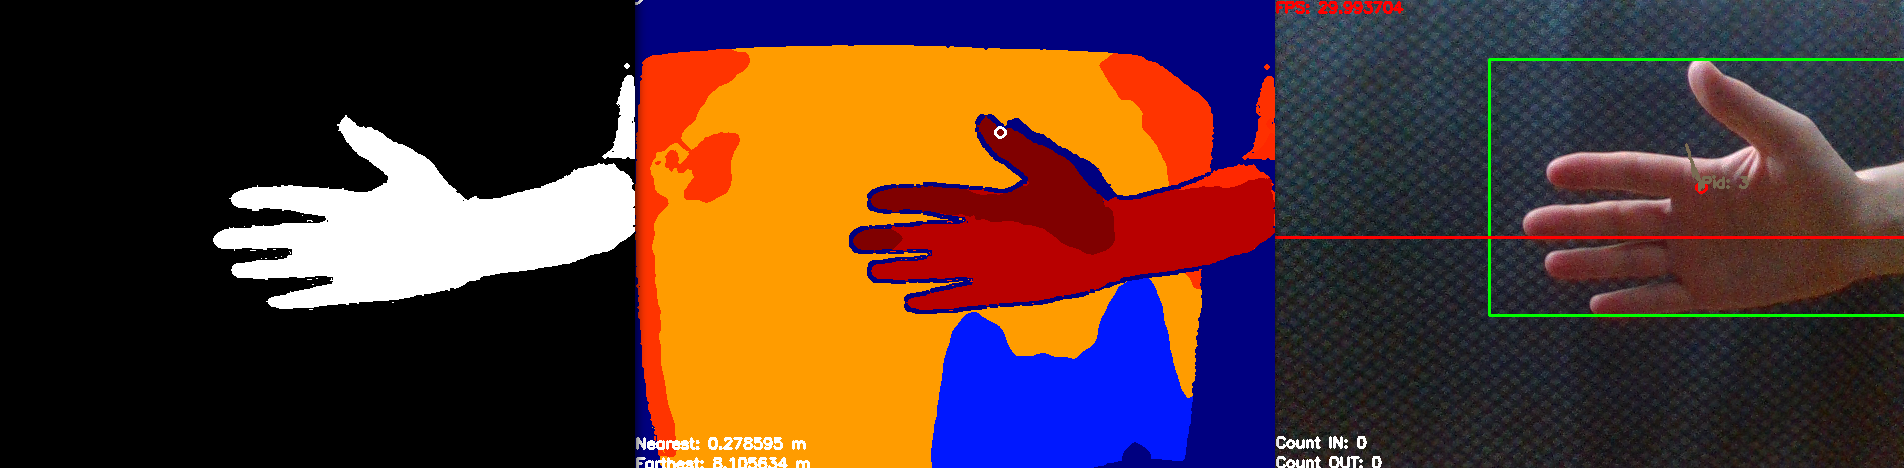
\includegraphics[width=\textwidth]{RSPCN.png}
  \caption{Esempio funzionamento Passenger Counter con telecamere RealSense.}
  \label{fig:RSPCN}
\end{figure}

Si noti che la lieve differenza nella posizione delle due telecamere fa in modo che il rettangolo che inscrive l'oggetto tracciato sia leggermente spostato rispetto all'oggetto, e cos\`\i\ pure il centro dell'oggetto, poich\`e il tracking viene effettuato sullo stream proveniente dalla telecamera a infrarossi, mentre il rettangolo viene disegnato sullo stream proveniente dalla telecamera a colori. 

Questo ovviamente non compromette la funzionalit\`a del programma ma pu\`o creare confusione durante la visualizzazione dei video.

%% Interruzione di pagina
\newpage

\subsection{Risultati ottenuti}
In questo parametro sono riportati i risultati dei test di funzionamento del contatore con telecamere RealSense. Si \`e cercato di replicare le stesse condizioni dei test effettuati con la versione a sottrazione del background. Ogni test \`e stato effettuato due volte per confrontare anche le prestazioni delle due telecamere.

\subsubsection{Dimostrazione funzionamento telecamera R200}
Nel seguito sono riportati alcuni fotogrammi tratti da una registrazione di un test del contatore. Per il test si \`e utilizzata la telecamera Intel RealSense R200, la quale \`e stata montata su uno stipite di una porta ad una altezza di circa 2,10m. Ogni frame riporta a sinistra l'immagine tratta dal video in ingresso dove sono state disegnate le forme per rendere pi\`u comprensibile il tracciamento, al centro l'immagine con le informazioni di profondit\`a(metodo \verb|getColorMap()|), a destra l'immagine cui sono state applicate le operazioni di soglia e sottrazione del rumore (metodo \verb|getFrame()|).

\begin{figure}[h!]
  \centering
  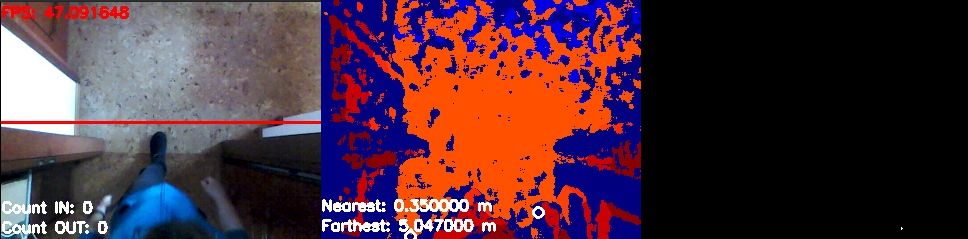
\includegraphics[width=\textwidth]{R2001.png}
  \caption{Risultato test RSPCN con telecamera R200: frame 1}
  \label{fig:R2001}
\end{figure}

\begin{figure}[h!]
  \centering
  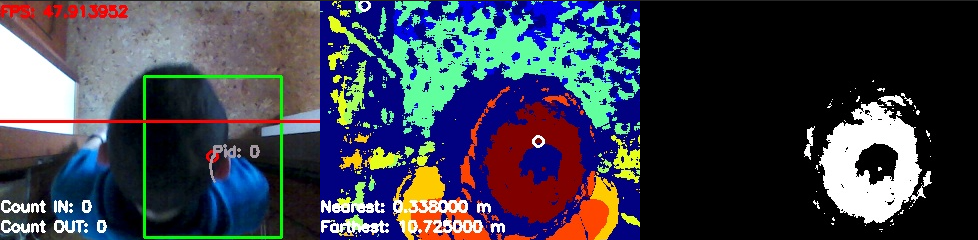
\includegraphics[width=\textwidth]{R2002.png}
  \caption{Risultato test RSPCN con telecamera R200: frame 2}
  \label{fig:R2002}
\end{figure}

Si noti ancora una volta come in figura \ref{fig:R2002} il rettangolo appare non centrato sulla testa del passeggero. Ci\`o \`e dovuto al fatto che la telecamera a colori e quelle a infrarossi hanno posizioni diverse.

Inoltre \`e opportuno notare come il centro della testa del passeggero, sempre in figura \ref{fig:R2002}, sia oscurato. Questo \`e devuto al fatto che il modello R200, poich\`e basato sulla visione stereoscopica, ha un range di funzionamento minimo molto elevato (30cm ca.) e, in questo caso, una parte della testa si trova fuori dal range operativo della telecamera.

%% Interruzione di pagina
\newpage

\begin{figure}[h!]
  \centering
  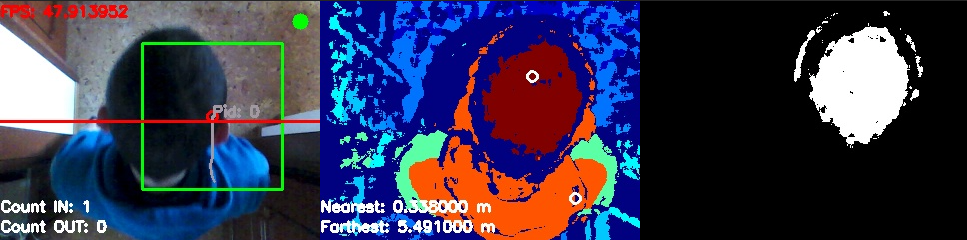
\includegraphics[width=\textwidth]{R2003.png}
  \caption{Risultato test RSPCN con telecamera R200: frame 3}
  \label{fig:R2003}
\end{figure}

In figura \ref{fig:R2003} il pallino verde in alto a destra nell'immagine indica la registrazione dell'evento di attraversamento della soglia.

\begin{figure}[h!]
  \centering
  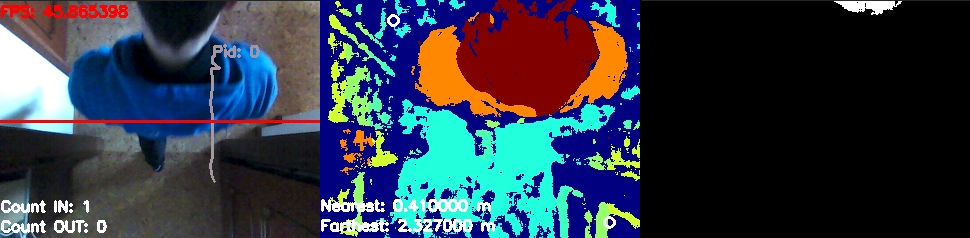
\includegraphics[width=\textwidth]{R2004.png}
  \caption{Risultato test RSPCN con telecamera R200: frame 4}
  \label{fig:R2004}
\end{figure}

%% Interruzione di pagina
\newpage

\subsubsection{Dimostrazione funzionamento telecamera SR300}
Nel seguito sono riportati alcuni fotogrammi tratti da una registrazione di un test del contatore. Per il test si \`e utilizzata la telecamera Intel RealSense SR300, la quale \`e stata montata su uno stipite di una porta ad una altezza di circa 2,10m. Il formato dei frame \`e lo stesso del caso precedente.

\begin{figure}[h!]
  \centering
  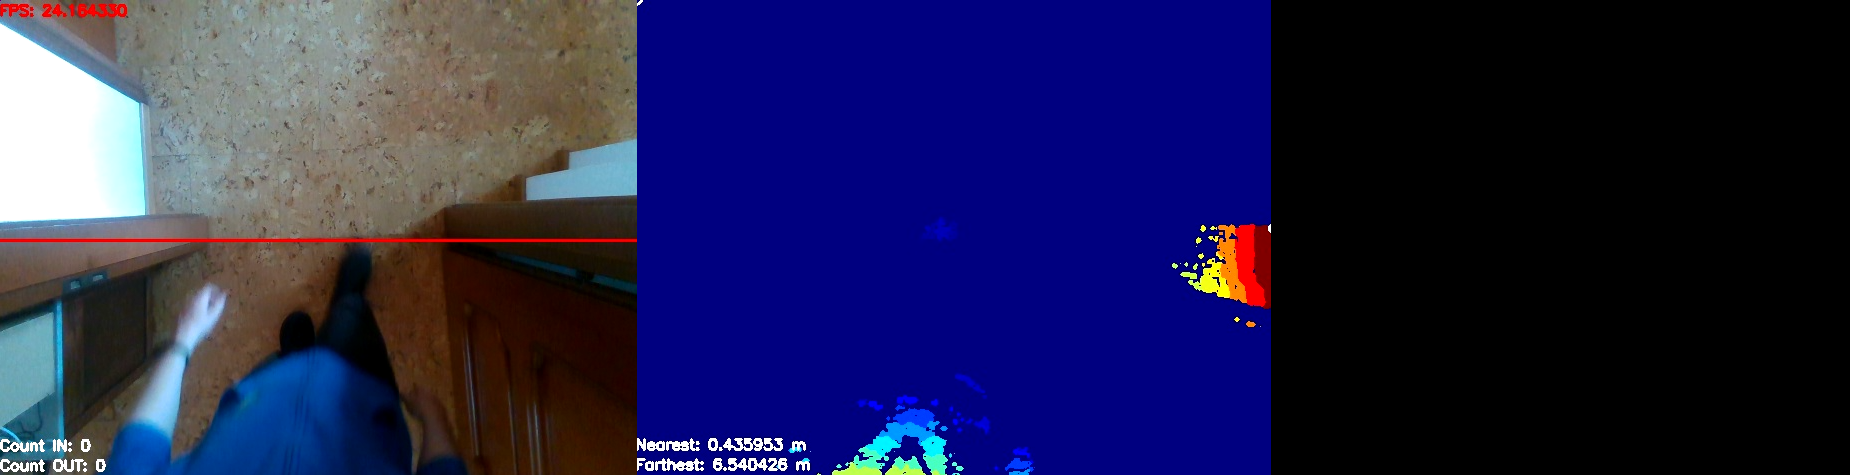
\includegraphics[width=\textwidth]{SR3001.png}
  \caption{Risultato test RSPCN con telecamera SR300: frame 1}
  \label{fig:SR3001}
\end{figure}

Si noti che in questo caso nell'immagine coi dati di profondit\`a non viene rilevato il pavimento. Questo \`e dovuto al fatto che il range operativo della telecamera SR300 \`e inferiore a quello della R200. Ci\`o per\`o non influisce sul corretto funzionamento del contatore.

\begin{figure}[h!]
  \centering
  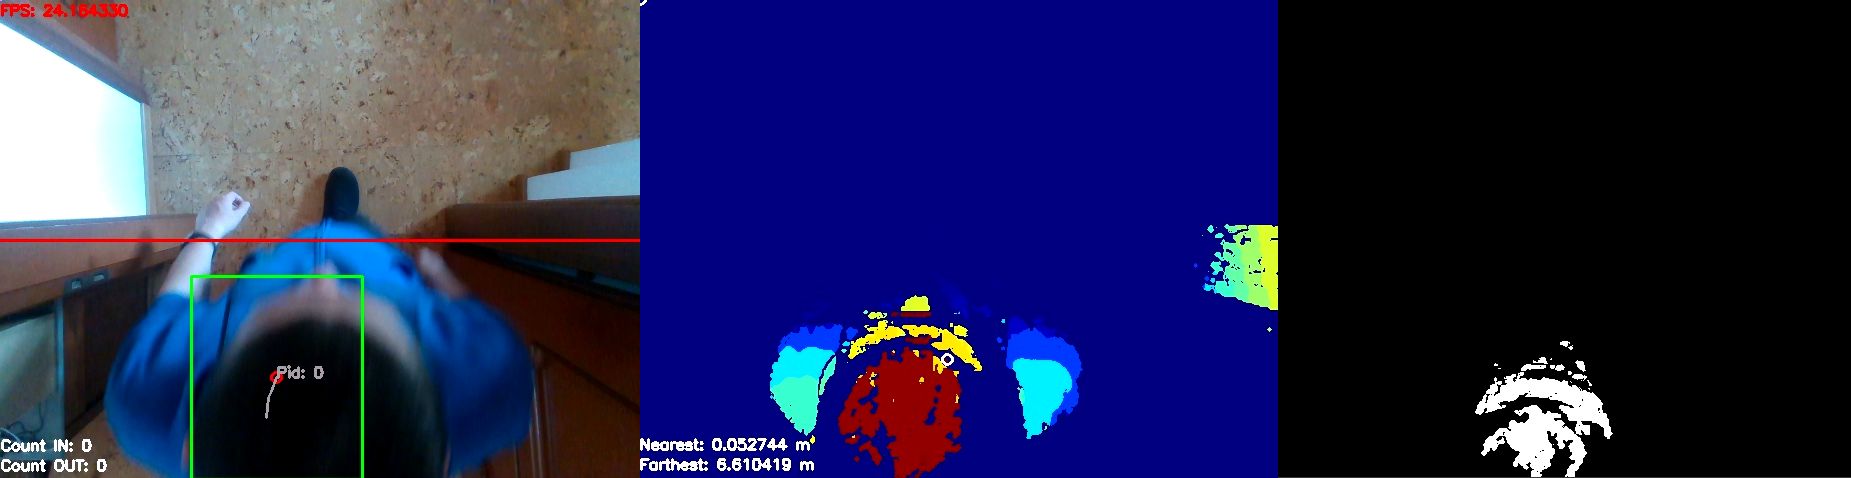
\includegraphics[width=\textwidth]{SR3002.png}
  \caption{Risultato test RSPCN con telecamera SR300: frame 2}
  \label{fig:SR3002}
\end{figure}

\begin{figure}[h!]
  \centering
  \includegraphics[width=\textwidth]{SR3003.png}
  \caption{Risultato test RSPCN con telecamera SR300: frame 3}
  \label{fig:SR3003}
\end{figure}

Si noti che, in questo caso, \`e stata rilevata correttamente l'intera testa del passeggero. Questo \`e dovuto al fatto che la telecamera SR300 ha un raggio minimo molto pi\`u basso poich\`e sfrutta la luce strutturata per ricostruire i dati di profondit\`a dell'immagine.

%% Interruzione di pagina
\newpage

\begin{figure}[h!]
  \centering
  \includegraphics[width=\textwidth]{SR3004.png}
  \caption{Risultato test RSPCN con telecamera SR300: frame 4}
  \label{fig:SR3004}
\end{figure}

%% Interruzione di pagina
\newpage

\subsubsection{Performance}
Per la misura dei tempi di esecuzione si \`e fatto uso della libreria standard \verb|chrono| di C++. I test sono stati effettuati usando le due telecamere RealSense su due diversi dispositivi: il ReliaGate 20-25 ed una macchina Linux ad alte prestazioni. I tempi sono stati mediati sul numero di cicli effettuati, cio\`e pari al numero di frame catturati dalla telecamera.

Nel seguito sono riportati i risultati relativi alle performance dell'applicazione utilizzando la telecamera RealSense SR300:

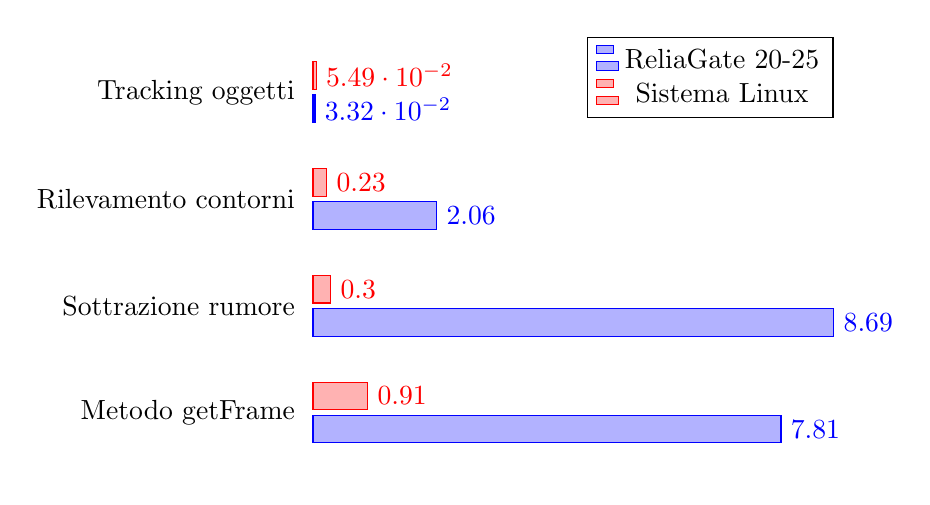
\begin{tikzpicture}
\begin{axis}[
  xbar,
  y axis line style = { opacity = 0 },
  axis x line       = none,
  tickwidth         = 0pt,
  enlarge y limits  = 0.2,
  enlarge x limits  = 0.02,
  symbolic y coords = {Metodo getFrame, Sottrazione rumore, Rilevamento contorni, Tracking oggetti},
  nodes near coords,
]
% ReliaGate 20-25
\addplot 
    coordinates {(7.80747,Metodo getFrame) (8.69046,Sottrazione rumore) (2.0645,Rilevamento contorni)
                    (0.033218,Tracking oggetti)};
% Sistema Linux
\addplot 
    coordinates {(0.913448,Metodo getFrame) (0.295688,Sottrazione rumore) (0.228186,Rilevamento contorni)
                    (0.054902,Tracking oggetti)};
\legend{ReliaGate 20-25, Sistema Linux}
\end{axis}
\end{tikzpicture}

\begin{table}[h!]
    \centering
	\begin{tabular}{|l|c|c|}
	\hline
    & ReliaGate 20-25 & Sistema Linux \\ \hline
    Tempo di esecuzione del loop principale & 37.1384 ms & 32.2761 ms \\ \hline
    Metodo getFrame & 7.80747 ms & 0.913448 ms \\ \hline
    Sottrazione del rumore & 8.69046 ms & 0.295688 ms \\ \hline
    Algoritmo rilevamento contorni & 2.0645 ms & 0.228186 ms \\ \hline
    Rilevamento e tracking degli oggetti & 0.033218 ms & 0.054902 ms \\ \hline
    Frame Rate & 30 FPS & 30 FPS \\ \hline
	\end{tabular}
    \caption{Performance Passenger Counter con telecamera RealSense SR300}
\end{table}

Anche in questo caso all'interno del tempo di esecuzione del loop principale \`e considerato il tempo speso ad attendere i frame dalla telecamera.

Nel seguito sono riportati i risultati relativi alle performance dell'applicazione utilizzando la telecamera RealSense R200:

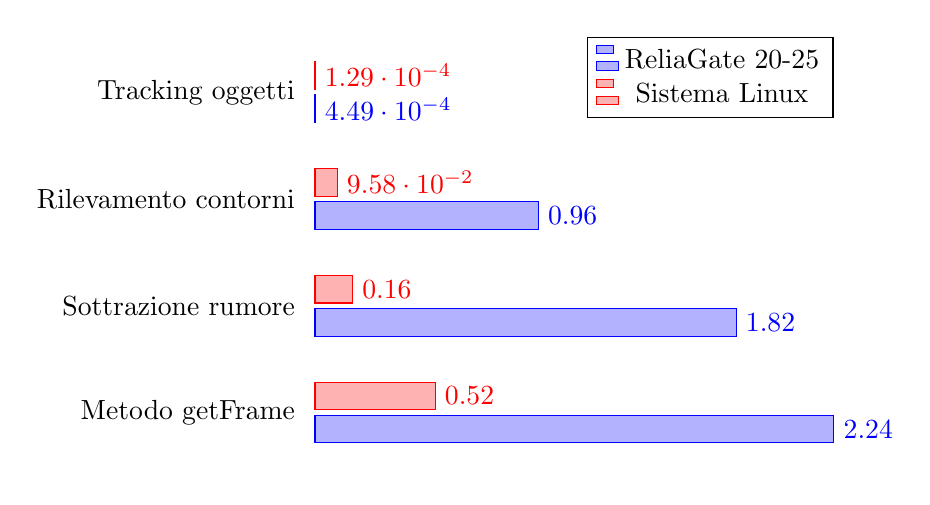
\begin{tikzpicture}
\begin{axis}[
  xbar,
  y axis line style = { opacity = 0 },
  axis x line       = none,
  tickwidth         = 0pt,
  enlarge y limits  = 0.2,
  enlarge x limits  = 0.02,
  symbolic y coords = {Metodo getFrame, Sottrazione rumore, Rilevamento contorni, Tracking oggetti},
  nodes near coords,
]
% ReliaGate 20-25
\addplot 
    coordinates {(2.23713,Metodo getFrame) (1.81564,Sottrazione rumore) (0.962472,Rilevamento contorni)
                    (4.48531e-4,Tracking oggetti)};
% Sistema Linux
\addplot 
    coordinates {(0.517965,Metodo getFrame) (0.162011,Sottrazione rumore) (0.095771,Rilevamento contorni)
                    (1.29373e-4,Tracking oggetti)};
\legend{ReliaGate 20-25, Sistema Linux}
\end{axis}
\end{tikzpicture}

%% Interruzione di pagina
\newpage

\begin{table}[h!]
    \centering
	\begin{tabular}{|l|c|c|}
	\hline
    & ReliaGate 20-25 & Sistema Linux \\ \hline
    Tempo di esecuzione del loop principale & 16.4351 ms & 15.8996 ms \\ \hline
    Metodo getFrame & 2.23713 ms & 0.517965 ms \\ \hline
    Sottrazione del rumore & 1.81564 ms & 0.162011 ms \\ \hline
    Algoritmo rilevamento contorni & 0.962472 ms & 0.095771 ms \\ \hline
    Rilevamento e tracking degli oggetti & 4.48531e-4 ms & 1.29373e-4 ms \\ \hline
    Frame Rate & 60 FPS & 60 FPS \\ \hline
	\end{tabular}
    \caption{Performance Passenger Counter con telecamera RealSense R200}
\end{table}

Come risulta evidente da queste tabelle i tempi di esecuzione sono molto migliorati rispetto al contatore a sottrazione del background. Ora il ReliaGate \`e in grado di mantenere il frame-rate stabile al valore impostato, ci\`o \`e dovuto al fatto che parte della computazione \`e stata spostata in hardware sull'ASIC delle telecamere.

Sempre grazie a questo fatto possiamo notare come i tempi di esecuzione del loop principale siano pressoch\'e identici per entrambi i sistemi, ora entrambi impiegano la maggior parte del tempo di CPU ad attendere il frame successivo in ingressso dalla telecamera (anche in questo caso il metodo \verb|wait_for_frames()| \`e bloccante).

%% Interruzione di pagina
\newpage

\subsection{Problemi}
Nonostante i miglioramenti anche questa versione del software non \`e esente da problemi, in questo caso sono pi\`u legati alle tecnologie impiegate.

Come riportato nella tabella \ref{table:SR300Spec} a pagina \pageref{table:SR300Spec} la telecamera SR300 ha un buon range di funzionamento, poich\`e basata sulla luce strutturata per il rilevamento dei dati di profondit\`a, ma non funziona in ambienti esterni. Ci\`o \`e dovuto al fatto che la luce infrarossa emessa dai proiettori della telecamera risulterebbero quasi invisibile sugli oggetti sui quali viene proiettata se presente la luce solare, la quale ha molte componenti infrarosse. Siccome l'ambito di applicazione del contatore \`e dato dai mezzi pubblici, ci si aspetta una illuminazione naturale abbastanza importante e ci\`o pu\`o compromettere notevolmente il funzionamento della telecamera.

La telecamera R200, i cui dati sono riportati nella tabella \ref{table:R200Spec} a pagina \pageref{table:R200Spec}, garantisce un buon funzionamento in ambiente outdoor poich\`e basata sulla visione stereoscopica invece che la luce strutturata. La luce solare in questo caso ne migliora il funzionamento invece che interferire. Purtroppo essendo basata sulla visione steroscopica il range di funzionamento \`e molto peggiore rispetto alla SR300 per il nostro caso applicativo. Dovendo installare la telecamera ad una altezza di 2,10m, il range minimo di 40cm genera problemi di rilevamento per tutti i passeggeri con una statura superiore al metro e ottanta. Infatti in figura \ref{fig:R2002} \`e possibile notare come parte della testa del passeggero risulti non rilevata correttamente. Nel caso questa area non rilevata fosse troppo ampia si perderebbero le capacit\`a di tracciare i passeggeri e quindi il funzionamento della telecamera risulterebbe compromesso.

Inoltre la telecamera R200 ha un FOV e una risoluzione leggermente inferiori alla telecamera SR300, ci\`o aumenta ulteriormente le difficolt\`a di tracciamento.

In conclusione possiamo affermare che entrambe le telecamere hanno dei difetti per l'applicazione considerata in questa tesi, comunque il funzionameno \`e molto migliore rispetto al caso del Passenger Counter a sottrazione del background e i punti di forza di questa tecnologia sono di gran lunga maggiori dei punti deboli.

%% Interruzione di pagina
\newpage

\section{Confronto implementazioni del Passenger Counter}
Nel corso della tesi sono state implementate diverse versioni del contatore, in diversi linguaggi. In questa sezione andremo ad analizzare quali sono queste implementazioni, come sono state realizzate  e quali sono le loro prestazioni.

Per brevit\`a nel seguito verranno adottate le seguenti abbreviazioni:
\begin{itemize}
\item BPC: Passenger Counter a sottrazione del background.
\item RPC: Passenger Counter con telecamere RealSense.
\end{itemize}

\subsection{Prestazioni}
Finora abbiamo trattato nel dettaglio le due diverse implementazioni del Passenger Counter. Ora confronteremo quali differenze comportano le diverse tecnologie ed algoritmi utilizzati del punto di vista delle prestazioni del programma.

\subsubsection{Costo computazionale}
L'algoritmo di sottrazione del background oltre ad essere impreciso \`e molto pesante dal punto di vista computazionale. L'aver spostato gran parte del lavoro sugli ASIC presenti nelle telecamere RealSense permette di avere uno stream in ingresso con un framerate molto pi\`u stabile ed elevato, inoltre permette di utilizzare molte pi\`u telecamere contemporaneamente.

Qui di seguito \`e riportato un confronto sui tempi di esecuzione delle funzioni principali delle due implementazioni del contatore. Per il confronto si \`e usata la telecamera SR300 e la webcam poich\`e hanno la stessa risoluzione e lo stesso framerate. I tempi riportati sono in millisecondi.

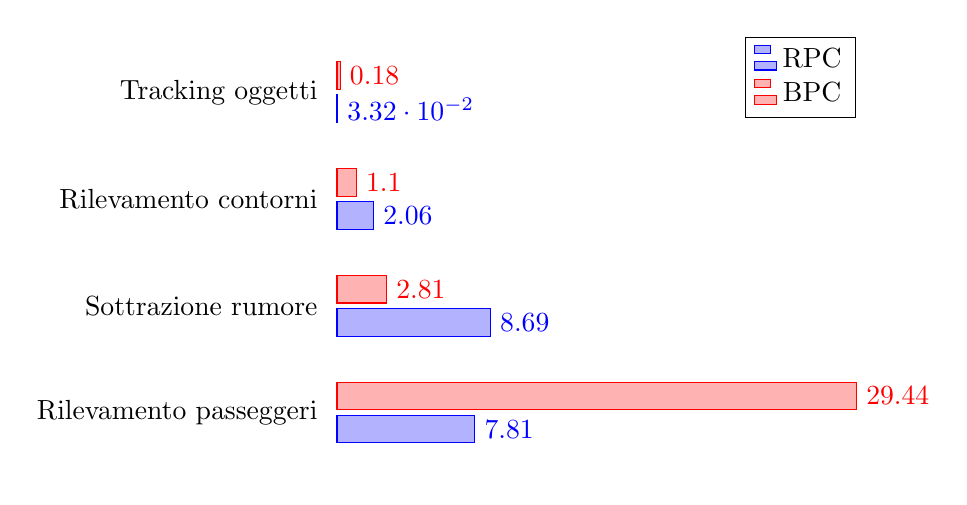
\begin{tikzpicture}
\begin{axis}[
  xbar,
  y axis line style = { opacity = 0 },
  axis x line       = none,
  tickwidth         = 0pt,
  enlarge y limits  = 0.2,
  enlarge x limits  = 0.02,
  symbolic y coords = {Rilevamento passeggeri, Sottrazione rumore, Rilevamento contorni, Tracking oggetti},
  nodes near coords,
]
% ReliaGate 20-25 RSPCN
\addplot 
    coordinates {(7.80747,Rilevamento passeggeri) (8.69046,Sottrazione rumore) (2.0645,Rilevamento contorni)
                    (0.033218,Tracking oggetti)};
% ReliaGate 20-25 BSPCN
\addplot 
    coordinates {(29.4414,Rilevamento passeggeri) (2.80683,Sottrazione rumore) (1.09507,Rilevamento contorni) 
                    (0.178409,Tracking oggetti)};
\legend{RPC, BPC}
\end{axis}
\end{tikzpicture}

%% Interruzione di pagina
\newpage

\subsubsection{Precisione nel tracciamento}
Le prestazioni del Passenger Counter a sottrazione del background sono di gran lunga peggiori dell'implementazione successiva. Il numero di falsi positivi nel tracciamento \`e molto maggiore del numero di oggetti tracciati correttamente.

\begin{figure}[h!]
\begin{minipage}[b]{8.5cm}
  \centering
  \includegraphics[width=8cm]{TrackBPC.png}
  \caption{Dettaglio tracking BPC}
  \label{fig:trackBPC}
\end{minipage}
\ \hspace{2mm} \hspace{3mm} \
\begin{minipage}[b]{8.5cm}
 \centering
  \includegraphics[width=8cm]{TrackRPC.png}
  \caption{Dettaglio tracking RPC}
  \label{fig:trackRPC}
\end{minipage}
\end{figure}

Il fatto che nel RPC venga tracciata solo la testa dei passeggeri permette un tracking molto pi\`u preciso. Infatti nel caso del BPC la forma del soggetto tracciato varia continuamente e, poich\`e il tracciamento \`e riferito al centro dell'area, ci\`o comporta un sacco di errori. In figura \ref{fig:trackBPC} possiamo notare come la traccia lasciata dal passeggero sia piena di discontinuit\`a e linee spezzate, d'altra parte in figura \ref{fig:trackRPC} la linea di tracciamento risulta molto pi\`u continua.

Inoltre bisogna tenere conto dei falsi positivi generati dalle ombre. Nel caso della sottrazione del background questo \`e un problema molto grave. Qui di seguito \`e riportato un confronto tra le due versioni.

\begin{figure}[h!]
\begin{minipage}[b]{8.5cm}
  \centering
  \includegraphics[width=8cm]{OmbraBPC.png}
  \caption{Dettaglio tracking ombra BPC}
  \label{fig:ombraBPC}
\end{minipage}
\ \hspace{2mm} \hspace{3mm} \
\begin{minipage}[b]{8.5cm}
 \centering
  \includegraphics[width=8cm]{OmbraRPC.png}
  \caption{Dettaglio tracking ombra RPC}
  \label{fig:ombraRPC}
\end{minipage}
\end{figure}

\subsubsection{Dipendenza dall'ambiente}
La versione a sottrazione del background ha una forte dipendenza dalle condizioni di luce. Variazioni troppo brusche nelle condizioni di illuminazione ne compromettono il funzionamento, essendo basato su un modello dello sfondo costante. Analogamente necessita che la telecamera sia montata su una struttura che non sia soggetta a vibrazioni. Nell'applicazione del sistema in un mezzo di trasporto ci\`o non \`e possibile mentre la versione RealSense del contatore \`e esente da entrambi questi problemi.

Infine, in condizioni di bassa illuminazione, il BPC si trova ad avere a che fare con un rumore molto elevato e quindi un degrado delle prestazioni. D'altro canto, essendo le telecamere RealSense dotate di proiettori di luce infrarossa, il RPC non risente di problemi di scarsa illuminazione e anzi, pi\`u l'ambiente \`e privo di luce migliore \`e il suo funzionamento.

\subsubsection{Raggio di azione}
L'implementazione con sottrazione del background non ha problemi legati al range di funzionamento, mentre le telecamere RealSense hanno un range piuttosto limitato e, nel caso della telecamra R200, ci\`o pu\`o compromettere il corretto funzionamento del programma.

Abbiamo visto infatti in figura \ref{fig:R2002} a pagina \pageref{fig:R2002} come l'eccessiva vicinanza dell'oggetto da tracciare non permetta alla telecamera di rilevare correttamente i dati di profondit\`a. Questo comporta un'area priva di dati al centro dell'oggetto da tracciare e, nel caso quest'area diventi troppo grande, un fallimento nel rilevamento dell'oggetto nell'immagine e/o un oggetto tracciato in modo non corretto.

\subsubsection{Costi}
Il contatore con sottrazione dello sfondo non \`e basato su nessun tipo di tecnologia particolare e pu\`o essere implementato con qualsiasi tipo di telecamera. L'RPC invece dipende dalle telecamere Intel RealSense, le quali hanno un costo pi\`u elevato di una semplice telecamera. Dal punto di vista dei costi di produzione questo \`e un grosso vantaggio.

Bisogna altres\`\i\ considerare il fatto che il BPC necessita di un hardware pi\`u potente, e quindi pi\`u costoso, a causa del suo costo computazionale pi\`u elevato.

\subsubsection{Conclusioni}
Poich\`e i vantaggi della versione con telecamere RealSense superano di gran lunga gli svantaggi, si \`e ritenuto opportuno utilizzare questa come versione principale del progetto. Nel seguito verranno trattati i vari porting e versioni del codice, tutte queste sono riferite alla versione con telecamere a infrarossi. La versione a sottrazione del background, a causa della sua imprecisione ed eccessivo costo computazionale, non \`e stata considerata meritevole di ulteriore attenzione e quindi accantonata in favore della versione RealSense. 

%% Interruzione di pagina
\newpage

\subsection{Versioni realizzate e porting}
Nel corso della tesi sono state realizzate molteplici versioni dello stesso codice. Il motivo principale per questi porting \`e stato quello di adattarsi al linguaggio di programmazione utilizzato maggiormente in Eurotech. Nel seguito analizzeremo le versioni del Passenger Counter con telecamere RealSense che sono state realizzate nel corso della tesi.

\subsubsection{Versione C++}
Il codice analizzato finora \`e riferito a questa versione del codice. Siccome OpenCV e la libreria RealSense sono scritte in questo linguaggio si \`e pensato di usare questo come punto di partenza. In seguito alla prima implementazione si \`e reso necessario il porting negli altri linguaggi per le motivazioni descritte in precedenza.

\subsubsection{Wrapping in Java}
Come primo passo si \`e deciso di effettuare un wrapping in Java del codice nativo sfruttando il tool open source \textbf{SWIG}\footnote{Pagina web del progetto: http://www.swig.org/}.

% TODO: Il seguente paragrafo \`e stato copiato spudoratamente. Cambiare.
SWIG (Simplified Wrapper and Interface Generator - Wrapper semplificato e generatore di interfacce) \`e un wrapper open source utilizzato per collegare i programmi per elaboratore o librerie scritte in C o C++ con altri linguaggi come C Sharp, Java, JavaScript, Go, Modula-3, OCaml, Octave, e Scheme.

L'obiettivo \`e quello di consentire la chiamata di funzioni native (C o C++) da altri linguaggi di programmazione, passando tipi di dati complessi, mantenendo la memoria libera, ereditariet\`a delle classi dei vari linguaggi, ecc. Il programmatore scrive un file di interfaccia che contiene un elenco di funzioni C/C++ che devono essere rese visibili ad un interprete. SWIG compila il file di interfaccia e genera normale C/C++ ed il codice nel linguaggio di programmazione di destinazione. SWIG generer\`a codice di conversione o serializzazione per le funzioni con argomenti semplici; il codice di conversione per i tipi complessi di argomenti deve essere scritto dal programmatore. Lo strumento SWIG crea codice sorgente che fornisce il collante tra C/C++ e il linguaggio di destinazione. A seconda del linguaggio software, questo collante \`e disponibile in due forme:

\begin{itemize}
\item una libreria condivisa che un interprete esistente pu\`o collegare come una qualche forma di modulo di estensione, o
\item una libreria condivisa che pu\`o essere collegata ad altri programmi compilati nel linguaggio di destinazione (ad esempio, utilizzando JNI in Java).
\end{itemize}

SWIG non viene utilizzato per chiamare le funzioni interpretate da codice nativo, questo deve essere fatto dal programmatore manualmente.

Questa versione conservava le prestazioni del codice nativo pur permettendo l'interfacciamento con Java. Si \`e comunque ritenuto necessario compiere un ulteriore passo ed effettuare il porting vero e proprio dell'applicazione in Java.

\subsubsection{Versione Java}
Il porting dell'applicazione ha comportato subito grossi problemi di compatibilit\`a poich\`e, bench\`e OpenCV avesse introdotto recentemente il supporto a Java, a causa della libreria librealsense \`e stato necessario appoggiarsi al progetto \textbf{JavaCPP}\footnote{Repository del progetto all'indirizzo: https://github.com/bytedeco/javacpp}.

JavaCPP \`e un progetto open source il cui obiettivo \`e fornire un accesso efficiente al codice nativo C++ dentro Java. Esso sfrutta le similitudini sintattiche e semantiche tra Java e C++ per raggiungere questo obiettivo. Sfrutta la Java Nativi Interface (JNI) quindi funziona per tutte le implementazioni di Java SE.

Praticamente, parsando il codice nativo degli header file delle librerie, realizza delle interfacce Java che permettono al codice Java di effettuare le chiamate delle librerie C++ installate sulla macchina host. Tramite questa pratica, i manutentori del progetto hanno prodotto delle interfacce complete per OpenCV, FFmpeg, libdc1394, PGR FlyCapture, OpenKinect, videoInput, ARToolKitPlus, e altri come parti del progetto \textbf{JavaCPP Presets}\footnote{Repository del progetto all'indirizzo: https://github.com/bytedeco/javacpp-presets}.

JavaCPP Presets \`e un sottoprogetto di JavaCPP il quale rende disponibile le interfacce verso le librerie C++ pi\`u usate prodotte usando JavaCPP. Esso rende quindi disponibili i file \verb|.jar| per l'interfacciamento alle librerie librealsense. 

Purtroppo questa interfaccia fa uso del progetto \textbf{JavaCV}\footnote{Repository del progetto all'indirizzo: https://github.com/bytedeco/javacv}, il quale \`e un wrapper Java di OpenCV realizzato sempre dal progetto JavaCPP sfruttando i preset resi disponibili da JavaCPP Presets. \`E stato quindi necessario utilizzare JavaCV al posto di OpenCV per realizzare questa versione del codice nonostante quest'ultimo disponesse di un suo interfacciamento a Java. \`E necessario notare per\`o che il progetto JavaCV \`e pi\`u vecchio dell'attuale interfacciamento ufficiale a Java di OpenCV e molto pi\`u completo della controparte. Nonostante ci\`o le differenze tra i due erano cos\`\i\ spiccate che \`e stata necessaria una revisione abbastanza corposa del codice e in alcuni casi non \`e stato possibile portare tutte le feature presenti nella versione C++.

Caratteristiche di questa implementazione:
\begin{itemize}
\item Utilizzo del framework Java per il display delle immagini al posto del modulo HighGui di OpenCV assente in questa versione della libreria.
\item Parallelizzazione della computazione affidata a Java
\item Aumento della portabili\`a del codice
\end{itemize}
Nonostante l'overhead computazionale dovuto all'interfacciamento Java, l'ottima parallelizzazione compiuta dalla Java Virtual Machine ha permesso una distribuzione del calcolo su tutti i thread disponibili sul ReliaGate che mitiga questo problema. Il codice cos\`\i\ realizzato quindi ha delle ottime performance anche su macchine poco prestanti.

%% Interruzione di pagina
\newpage

Qui di seguito sono riportati i dati dei tempi di esecuzione delle funzioni principali del Passenger Counter con telecamere RealSense in Java. I dati sono riferiti all'uso della telecamera R200 sul ReliaGate 20-25.

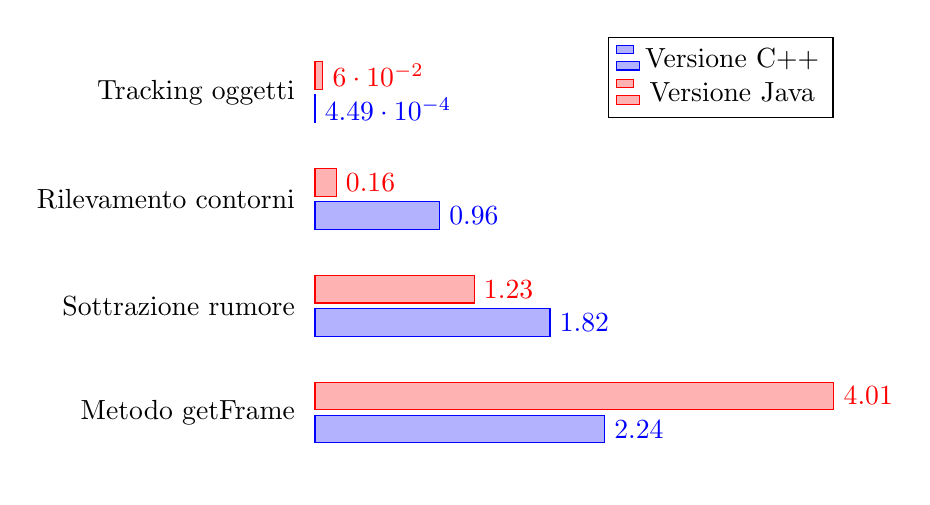
\begin{tikzpicture}
\begin{axis}[
  xbar,
  y axis line style = { opacity = 0 },
  axis x line       = none,
  tickwidth         = 0pt,
  enlarge y limits  = 0.2,
  enlarge x limits  = 0.02,
  symbolic y coords = {Metodo getFrame, Sottrazione rumore, Rilevamento contorni, Tracking oggetti},
  nodes near coords,
]
% ReliaGate 20-25 C++
\addplot 
    coordinates {(2.23713,Metodo getFrame) (1.81564,Sottrazione rumore) (0.962472,Rilevamento contorni)
                    (4.48531e-4,Tracking oggetti)};
% ReliaGate 20-25 Java
\addplot 
    coordinates {(4.008504,Metodo getFrame) (1.230020,Sottrazione rumore) (0.163716,Rilevamento contorni)
                    (0.059985,Tracking oggetti)};
\legend{Versione C++, Versione Java}
\end{axis}
\end{tikzpicture}

\begin{table}[h!]
    \centering
	\begin{tabular}{|l|c|c|}
	\hline
    & Versione C++ & Versione Java \\ \hline
    Tempo di esecuzione del loop principale & 16.4351 ms & 16.932457 ms \\ \hline
    Metodo getFrame & 2.23713 ms & 4.008504 ms \\ \hline
    Sottrazione del rumore & 1.81564 ms & 1.230020 ms \\ \hline
    Algoritmo rilevamento contorni & 0.962472 ms & 0.163716 ms \\ \hline
    Rilevamento e tracking degli oggetti & 4.48531e-4 ms & 0.059985 ms \\ \hline
    Frame Rate & 60 FPS & 60 FPS \\ \hline
	\end{tabular}
    \caption{Confronto performance versioni Passenger Counter con telecamera R200.}
\end{table}

\subsubsection{Versione OSGi}
\textbf{In pausa finch\`e non siamo sicuri di implementarla.}

%% Interruzione di pagina
\newpage

\section{Piattaforma Yocto: realizzazione e features}
In questa sezione tratteremo la distribuzione Linux, realizzata per mezzo del progetto Yocto, a supporto degli applicativi trattati nelle sezioni precedenti. Vedremo quali sono le sue caratteristiche, come \`e stata realizzata e i problemi riscontrati nella sua realizzazione.

\subsection{Caratteristiche della distribuzione}
Il risultato finale di quanto si \`e realizzato \`e riportato in figura \ref{fig:SWStack}.

\begin{figure}[h!]
  \centering
  \includegraphics[width=\textwidth]{SoftwareStackDiag.png}
  \caption{Diagramma dello stack software della distribuzione realizzata}
  \label{fig:SWStack}
\end{figure}

La distribuzione \`e formata da quattro parti fondamentali:

\begin{enumerate}
\item Poky: la reference distribution del progetto Yocto. Fa da template per la costruzione della propria distro Linux customizzata. Nel progetto si \`e usata la versione 2.2 - Morty a causa delle restrizioni dovute alle librerie RealSense.
\item OpenCV: come visto in precedenza, fondamentale per l'image processing.
\item librealsense: necessaria per l'interfacciamento con le telecamere RealSense.
\item OpenJDK 8: necessario per l'esecuzione delle versioni basate su Java del Passenger Counter.
\end{enumerate}

%% Interruzione di pagina
\newpage

\subsection{Build System di Yocto}
Come spiegato nella sezione \ref{Yocto} a pagina \pageref{Yocto}, il progetto Yocto \`e basato su "ricette". Queste ricette contengono dei metadati con le istruzioni su come installare il software nella distribuzione da realizzare. Ogni ricetta esegue le seguenti operazioni in ordine:

\begin{enumerate}
\item Scarica i sorgenti del software.
\item Effettua la cross-compilazione dei sorgenti.
\item Realizza un pacchetto (.rpm, .deb, a seconda delle impostazioni).
\item Installa il pacchetto software nella distribuzione.
\end{enumerate}

Una volta scaricate ed installate nella distribuzione tutte le ricette, viene creata l'immagine del sistema operativo che pu\`o essere scritta su un supporto di memoria e caricata sull'hardware.

Il build system di Yocto \`e organizzato come segue: la directory principale \`e data dalla distribuzione template Poky. Al suo interno sono presenti i layer fondamentali per la costruzione della distribuzione template e qui andranno scaricati i layer per le ricette aggiuntive. All'interno di questa directory verr\`a creata la Build Directory, la quale contiene i file di configurazione del processo di build e conterr\`a l'immagine finale della distribuzione.

\begin{figure}[h!]
  \centering
  \includegraphics[scale=0.6]{YoctoDirectory.png}
  \caption{Struttura della directory di lavoro del progetto Yocto}
  \label{fig:YoctoDirectory}
\end{figure}

%% Interruzione di pagina
\newpage

\subsubsection{bitbake}
This directory includes a copy of BitBake for ease of use. The copy usually matches the current stable BitBake release from the BitBake project. BitBake, a Metadata interpreter, reads the Yocto Project Metadata and runs the tasks defined by that data. Failures are usually from the Metadata and not from BitBake itself. Consequently, most users do not need to worry about BitBake.

When you run the bitbake command, the main BitBake executable, which resides in the bitbake/bin/ directory, starts. Sourcing an environment setup script (e.g. oe-init-build-env or oe-init-build-env-memres) places the scripts and bitbake/bin directories (in that order) into the shell's PATH environment variable.

\subsubsection{build}
This directory contains user configuration files and the output generated by the OpenEmbedded build system in its standard configuration where the source tree is combined with the output. The Build Directory is created initially when you source the OpenEmbedded build environment setup script (i.e. oe-init-build-env or oe-init-build-env-memres).

It is also possible to place output and configuration files in a directory separate from the Source Directory by providing a directory name when you source the setup script. For information on separating output from your local Source Directory files, see the "oe-init-build-env and "oe-init-build-env-memres" sections.

Le preferenze circa il software da installare nella distribuzione e il processo di build vanno specificate in due file di configurazione della Build Directory:

\begin{itemize}
\item \textbf{local.conf}: local.conf file contains documentation on the various configuration options. Any variable set here overrides any variable set elsewhere within the environment unless that variable is hard-coded within a file (e.g. by using '=' instead of '?='). Some variables are hard-coded for various reasons but these variables are relatively rare.

Edit this file to set the \verb|MACHINE| for which you want to build, which package types you wish to use (\verb|PACKAGE_CLASSES|), and the location from which you want to access downloaded files (\verb|DL_DIR|).

If local.conf is not present when you start the build, the OpenEmbedded build system creates it from local.conf.sample when you source the top-level build environment setup script (i.e. oe-init-build-env or oe-init-build-env-memres).

The source local.conf.sample file used depends on the \verb|$TEMPLATECONF| script variable, which defaults to meta-poky/conf when you are building from the Yocto Project development environment and defaults to meta/conf when you are building from the OpenEmbedded Core environment. Because the script variable points to the source of the local.conf.sample file, this implies that you can configure your build environment from any layer by setting the variable in the top-level build environment setup script as follows:

     \verb|TEMPLATECONF=your_layer/conf|
            
Once the build process gets the sample file, it uses sed to substitute final \verb|${OEROOT}| values for all \verb|##OEROOT##| values.
\item \textbf{bblayers.conf}: This configuration file defines layers, which are directory trees, traversed (or walked) by BitBake. The bblayers.conf file uses the BBLAYERS variable to list the layers BitBake tries to find.

If bblayers.conf is not present when you start the build, the OpenEmbedded build system creates it from bblayers.conf.sample when you source the top-level build environment setup script (i.e. oe-init-build-env or oe-init-build-env-memres).

The source bblayers.conf.sample file used depends on the \verb|$TEMPLATECONF| script variable, which defaults to meta-poky/conf when you are building from the Yocto Project development environment and defaults to meta/conf when you are building from the OpenEmbedded Core environment. Because the script variable points to the source of the bblayers.conf.sample file, this implies that you can base your build from any layer by setting the variable in the top-level build environment setup script as follows:

     \verb|TEMPLATECONF=your_layer/conf|
            
Once the build process gets the sample file, it uses sed to substitute final \verb|${OEROOT}| values for all \verb|##OEROOT##| values.
\end{itemize}

\subsubsection{documentation}
This directory holds the source for the Yocto Project documentation as well as templates and tools that allow you to generate PDF and HTML versions of the manuals. Each manual is contained in a sub-folder. For example, the files for this manual reside in the ref-manual/ directory.

\subsubsection{meta}
This directory contains the OpenEmbedded Core metadata. The directory holds recipes, common classes, and machine configuration for emulated targets (qemux86, qemuarm, and so forth.)
Ad esempio all'interno di questa cartella \`e presente la folder meta/recipes-sato, la quale contiene Sato demo/reference UI/UX and its associated applications and configuration data.

\subsubsection{meta-yocto}
This directory contains the configuration for the Poky reference distribution.

\subsubsection{meta-yocto-bsp}
This directory contains the Yocto Project reference hardware Board Support Packages (BSPs). For more information on BSPs, see the Yocto Project Board Support Package (BSP) Developer's Guide.

\subsubsection{meta-selftest}
This directory adds additional recipes and append files used by the OpenEmbedded selftests to verify the behavior of the build system.

You do not have to add this layer to your bblayers.conf file unless you want to run the selftests.

\subsubsection{meta-skeleton}
This directory contains template recipes for BSP and kernel development.

\subsubsection{scripts}
This directory contains various integration scripts that implement extra functionality in the Yocto Project environment (e.g. QEMU scripts). The oe-init-build-env and oe-init-build-env-memres scripts append this directory to the shell's PATH environment variable.

The scripts directory has useful scripts that assist in contributing back to the Yocto Project, such as create-pull-request and send-pull-request.

\subsubsection{oe-init-build-env}
This script is one of two scripts that set up the OpenEmbedded build environment. For information on the other script, see the "oe-init-build-env-memres" section.

Running this script with the source command in a shell makes changes to PATH and sets other core BitBake variables based on the current working directory. You need to run an environment setup script before running BitBake commands. The script uses other scripts within the scripts directory to do the bulk of the work.

When you run this script, your Yocto Project environment is set up, a Build Directory is created, your working directory becomes the Build Directory, and you are presented with a list of common BitBake targets. Here is an example:

\begin{lstlisting}
\verb|$| source oe-init-build-env

### Shell environment set up for builds. ###

You can now run 'bitbake <target>'

Common targets are:
    core-image-minimal
    core-image-sato
    meta-toolchain
    adt-installer
    meta-ide-support

You can also run generated qemu images with a command like 'runqemu qemux86'
\end{lstlisting}
            
The script gets its default list of common targets from the conf-notes.txt file, which is found in the meta-yocto directory within the Source Directory. Should you have custom distributions, it is very easy to modify this configuration file to include your targets for your distribution. See the "Creating a Custom Template Configuration Directory" section in the Yocto Project Development Manual for more information.

By default, running this script without a Build Directory argument creates the build directory in your current working directory. If you provide a Build Directory argument when you source the script, you direct the OpenEmbedded build system to create a Build Directory of your choice. For example, the following command creates a Build Directory named mybuilds that is outside of the Source Directory:

\begin{lstlisting}
\verb|$| source oe-init-build-env ~/mybuilds
\end{lstlisting}
            
The OpenEmbedded build system uses the template configuration files, which are found by default in the meta-yocto/conf directory in the Source Directory. See the "Creating a Custom Template Configuration Directory" section in the Yocto Project Development Manual for more information.

\subsubsection{oe-init-build-env-memres}
This script is one of two scripts that set up the OpenEmbedded build environment. Aside from setting up the environment, this script starts a memory-resident BitBake server. For information on the other setup script, see the "oe-init-build-env" section.

Memory-resident BitBake resides in memory until you specifically remove it using the following BitBake command:

\begin{lstlisting}
\verb|$| bitbake -m
\end{lstlisting}
            
Running this script with the source command in a shell makes changes to PATH and sets other core BitBake variables based on the current working directory. One of these variables is the BBSERVER variable, which allows the OpenEmbedded build system to locate the server that is running BitBake.

You need to run an environment setup script before using BitBake commands. Following is the script syntax:

\begin{lstlisting}
\verb|$| source oe-init-build-env-memres port_number build_dir
\end{lstlisting}
            
The script uses other scripts within the scripts directory to do the bulk of the work.

If you do not provide a port number with the script, the BitBake server starts at a randomnly selected port.

When you run this script, your Yocto Project environment is set up, a Build Directory is created, your working directory becomes the Build Directory, and you are presented with a list of common BitBake targets. Here is an example:

\begin{lstlisting}
\verb|$| source oe-init-build-env-memres
No port specified, using dynamically selected port

### Shell environment set up for builds. ###

You can now run 'bitbake <target>'

Common targets are:
    core-image-minimal
    core-image-sato
    meta-toolchain
    adt-installer
    meta-ide-support

You can also run generated qemu images with a command like 'runqemu qemux86'
Bitbake server started on demand as needed, use bitbake -m to shut it down
\end{lstlisting}
            
The script gets its default list of common targets from the conf-notes.txt file, which is found in the meta-yocto directory within the Source Directory. Should you have custom distributions, it is very easy to modify this configuration file to include your targets for your distribution. See the "Creating a Custom Template Configuration Directory" section in the Yocto Project Development Manual for more information.

By default, running this script without a Build Directory argument creates a build directory named build. If you provide a Build Directory argument when you source the script, the Build Directory is created using that name. For example, the following command starts the BitBake server using a randomnly selected port and creates a Build Directory named mybuilds that is outside of the Source Directory:

\begin{lstlisting}
\verb|$| source oe-init-build-env-memres ~/mybuilds
\end{lstlisting}
            
The OpenEmbedded build system uses the template configuration files, which are found by default in the meta-yocto/conf directory in the Source Directory. See the "Creating a Custom Template Configuration Directory" section in the Yocto Project Development Manual for more information.

\subsubsection{LICENSE, README, and README.hardware}
These files are standard top-level files.

%% Interruzione di pagina
\newpage

\subsection{Realizzazione}
Lo sviluppo della distribuzione \`e stato parallelo allo sviluppo dell'applicazione. Mano a mano che si aggiungevano componenti aumentavano i requisiti dell'applicativo e di conseguenza venivano aggiunte parti alla distro. Ci\`o significava aggiungere gradualmente nuovi layer e nuove ricette al build system.

Per lo sviluppo del progetto sono state realizzate principalmente tre versioni della distribuzione, verranno analizzate nel seguito in ordine cronologico.

\subsubsection{Prima versione}
La prima versione \`e stata realizzata per supportare l'applicazione del Passenger Counter a sottrazione del background, quindi prevedeva solamente l'installazione di OpenCV sul ReliaGate 20-25. Per questa versione sono stati aggiunti solamente due layer alla configurazione standard di Poky:

\begin{itemize}
\item \textbf{meta-intel}: layer contenente metadati per il supporto di hardware intel. Questo layer \`e necessario per poter targettare correttamente il processore Intel sul quale \`e basato il ReliaGate 20-25.
\item \textbf{meta-openembedded}: \`e un layer contenente una collezione di layer dove sono riportate le ricette per i software pi\`u comuni. Questo layer era necessario in quanto contiene le ricette per l'installazione di OpenCV.
\end{itemize}

Poich\`e non vi erano problemi di compatibilit\`a fra i layer \`e stato possibile installare l'ultima versione disponibile di tutto il software. Quindi in questa versione della distribuzione era disponibile OpenCV 3.2.

Inoltre, per visualizzare le finestre di OpenCV contenenti gli stream video dalle telecamere, era necessario disporre del Window System X11. Per questo motivo si \`e deciso di installare la Sato reference User Interface, resa disponibile dal layer \textbf{openembedded-core}, fornito assieme a Poky. Questa interfaccia utente \`e basata su GTK+ e rende disponibile X11.

\subsubsection{Seconda versione}
Questa versione \`e stata realizzata per supportare il Passenger Counter con telecamere RealSense. Per poter installare correttamente le librerie librealsense e i driver delle telecamere \`e stato necessario aggiungere un nuovo layer: \textbf{meta-intel-realsense}.

Purtroppo questo layer risultava essere compatibile solamente con la versione 4.8 del kernel Linux, contenuta nella versione Morty di Poky. \`E stato quindi necessario effettuare un downgrade della versione di Poky con conseguente downgrade della versione di OpenCV. In questa versione della distribuzione erano quindi presenti OpenCV 3.1 e la libreria librealsense 1.12.1.

Il downgrade di OpenCV ha richiesto qualche accorgimento in fase di cross-compilazione del Passenger Counter in quanto la versione 3.2 di OpenCV aveva ridotto il numero di moduli, integrando pi\`u funzionalit\`a in uno stesso modulo.

\subsubsection{Terza versione}
Questa versione \`e stata realizzata per supportare il Passenger Counter con telecamere RealSense e le varie versioni Java. Ci\`o ha significato installare una Java Run-time Environment e un JDK. Si \`e scelto di installare OpenJDK-8 perch\`e il processo di installazione era pi\`u semplice. Sono infatti noti dei problemi di installazione per la versione Oracle del JDK.

\`E stato quindi necesario installare un nuovo layer: \textbf{meta-java}. Purtroppo il versioning di questo layer non seguiva lo standard dei restanti layer e mostrava problemi di compatibilit\`a con gli altri layer. \`E stato necessario percorrere all'indietro lo storico dei commit della repository contenente il layer, fino a trovare una versione compatibile con l'immagine realizzata finora.

Poich\`e si voleva rendere disponibile la API Java ufficiale di OpenCV \`e stato necessario modificare a mano la ricetta di OpenCV in quanto solo l'ultima versione di detta ricetta si occupava di generare tale API. Usando una versione pi\`u vecchia, per i problemi di compatibilit\`a delle librerie RealSense, la API non veniva generata.

Lo stack software completo di questa versione della distribuzione \`e riportato in figura \ref{fig:SWStack} ed \`e la versione finale della distribuzione.

%% Interruzione di pagina
\newpage

\subsection{File di configurazione: local.conf}
Qui di seguito riportiamo il file di configurazione della versione finale della distribuzione.

\begin{lstlisting}[caption=local.conf]
MACHINE ??= "intel-corei7-64"
DISTRO ?= "poky"
PACKAGE_CLASSES ?= "package_rpm"
SDKMACHINE ?= "x86_64"
EXTRA_IMAGE_FEATURES ?= "debug-tweaks"

USER_CLASSES ?= "buildstats image-mklibs image-prelink"
PATCHRESOLVE = "noop"
BB_DISKMON_DIRS = "\
    STOPTASKS,${TMPDIR},1G,100K \
    STOPTASKS,${DL_DIR},1G,100K \
    STOPTASKS,${SSTATE_DIR},1G,100K \
    STOPTASKS,/tmp,100M,100K \
    ABORT,${TMPDIR},100M,1K \
    ABORT,${DL_DIR},100M,1K \
    ABORT,${SSTATE_DIR},100M,1K \
    ABORT,/tmp,10M,1K"

PACKAGECONFIG_append_pn-qemu-native = " sdl"
PACKAGECONFIG_append_pn-nativesdk-qemu = " sdl"

CONF_VERSION = "1"

BB_NUMBER_THREADS = '12'
PARALLEL_MAKE = '-j 12'

# Java installation
IMAGE_INSTALL_append = " openjdk-8 "
PREFERRED_PROVIDER_virtual/java-initial-native = "cacao-initial-native"
PREFERRED_PROVIDER_virtual/java-native = "jamvm-native"
PREFERRED_PROVIDER_virtual/javac-native = "ecj-bootstrap-native"

# OpenCV installation
CORE_IMAGE_EXTRA_INSTALL += "opencv opencv-samples libopencv-core-dev libopencv-highgui-dev libopencv-imgproc-dev libopencv-objdetect-dev libopencv-ml-dev"
\end{lstlisting}

Questo \`e il file principale per la configurazione della build. Come detto in precedenza contiene le istruzioni su quali software installare e altri metadati sul processo di build. 

%% Interruzione di pagina
\newpage

Vediamo ora nel dettaglio il significato di questi parametri:

\begin{itemize}
\item \verb|MACHINE|: Specifies the target device for which the image is built. The variable corresponds to a machine configuration file of the same name, through which machine-specific configurations are set. Thus, when MACHINE is set to "qemux86" there exists the corresponding qemux86.conf machine configuration file, which can be found in the Source Directory in meta/conf/machine. Nel nostro caso stiamo costruendo una distribuzione per una architettura Intel 64-bit.
\item \verb|DISTRO|: The short name of the distribution. This variable corresponds to a distribution configuration file whose root name is the same as the variable's argument and whose filename extension is .conf. For example, the distribution configuration file for the Poky distribution is named poky.conf and resides in the meta-poky/conf/distro directory of the Source Directory. 
\item \verb|PACKAGE_CLASSES|: specifies the package manager the OpenEmbedded build system uses when packaging data.
\item \verb|SDKMACHINE|: The machine for which the SDK is built. In other words, the SDK is built such that it runs on the target you specify with the SDKMACHINE value. The value points to a corresponding .conf file under conf/machine-sdk/. You can use "\verb|i686|" and "\verb|x86_64|" as possible values for this variable. The variable defaults to "\verb|i686|" and is set in the local.conf file in the Build Directory.
\item \verb|EXTRA_IMAGE_FEATURES|: A list of additional features to include in an image. "debug-tweaks" - Makes an image suitable for debugging. For example, allows root logins without passwords and enables post-installation logging.
\item \verb|PATCHRESOLVE|: Determines the action to take when a patch fails. 
\item \verb|BB_DISKMON_DIRS|: Monitors disk space and available inodes during the build and allows you to control the build based on these parameters.
\item \verb|BB_NUMBER_THREADS|: The maximum number of tasks BitBake should run in parallel at any one time. The OpenEmbedded build system automatically configures this variable to be equal to the number of cores on the build system. For example, a system with a dual core processor that also uses hyper-threading causes the \verb|BB_NUMBER_THREADS| variable to default to "4".
\item \verb|PARALLEL_MAKE|: Extra options passed to the make command during the \verb|do_compile| task in order to specify parallel compilation on the local build host. This variable is usually in the form "-j x", where x represents the maximum number of parallel threads make can run.
\item \verb|IMAGE_INSTALL|: Specifies the packages to install into an image.
\item \verb|CORE_IMAGE_EXTRA_INSTALL|: Specifies the list of packages to be added to the image.
\end{itemize}

%% Interruzione di pagina
\newpage

Si noti la mancanza della libreria RealSense tra i pacchetti installati nella distribuzione. Questo \`e dovuto al fatto che la sua installazione avviene usando un secondo file di configurazione "auto.conf", come specificato nelle istruzioni di installazione della libreria.

\begin{lstlisting}[caption=auto.conf]
require include/intel-librealsense.inc

# Intel Realsense
CORE_IMAGE_EXTRA_INSTALL += "librealsense-graphical-examples"
\end{lstlisting}

La keyword \verb|require| va a prendere la ricetta specificata nel seguito, necessaria all'installazione della libreria.

\subsection{Modifica alla ricetta di OpenCV}
Per aggiungere le API Java di OpenCV \`e stato necessario modificare la ricetta di OpenCV come segue:

\begin{lstlisting}[language=diff]
...
- PACKAGECONFIG ??= "eigen jpeg png tiff v4l libv4l gstreamer samples tbb gphoto2 \
+ PACKAGECONFIG ??= "eigen jpeg png tiff v4l libv4l gstreamer samples tbb java gphoto2 \
    ${@bb.utils.contains("DISTRO_FEATURES", "x11", "gtk", "", d)} \
    ${@bb.utils.contains("LICENSE_FLAGS_WHITELIST", "commercial", "libav", "", d)}"
...
PACKAGECONFIG[jasper] = "-DWITH_JASPER=ON,-DWITH_JASPER=OFF,jasper,"
+ PACKAGECONFIG[java] = "-DJAVA_INCLUDE_PATH=${JAVA_HOME}/include -DJAVA_INCLUDE_PATH2=${JAVA_HOME}/include/linux -DJAVA_AWT_INCLUDE_PATH=${JAVA_HOME}/include -DJAVA_AWT_LIBRARY=${JAVA_HOME}/lib/amd64/libjawt.so -DJAVA_JVM_LIBRARY=${JAVA_HOME}/lib/amd64/server/libjvm.so,,ant-native fastjar-native openjdk-8-native,"
PACKAGECONFIG[jpeg] = "-DWITH_JPEG=ON,-DWITH_JPEG=OFF,jpeg,"
...
PACKAGECONFIG[opencl] = "-DWITH_OPENCL=ON,-DWITH_OPENCL=OFF,opencl-headers,"
- PACKAGECONFIG[oracle-java] = "-DJAVA_INCLUDE_PATH=${JAVA_HOME}/include -DJAVA_INCLUDE_PATH2=${JAVA_HOME}/include/linux -DJAVA_AWT_INCLUDE_PATH=${JAVA_HOME}/include -DJAVA_AWT_LIBRARY=${JAVA_HOME}/lib/amd64/libjawt.so -DJAVA_JVM_LIBRARY=${JAVA_HOME}/lib/amd64/server/libjvm.so,,ant-native oracle-jse-jdk oracle-jse-jdk-native,"
+ PACKAGECONFIG[oracle-java] = "-DJAVA_INCLUDE_PATH=${ORACLE_JAVA_HOME}/include -DJAVA_INCLUDE_PATH2=${ORACLE_JAVA_HOME}/include/linux -DJAVA_AWT_INCLUDE_PATH=${ORACLE_JAVA_HOME}/include -DJAVA_AWT_LIBRARY=${ORACLE_JAVA_HOME}/lib/amd64/libjawt.so -DJAVA_JVM_LIBRARY=${ORACLE_JAVA_HOME}/lib/amd64/server/libjvm.so,,ant-native oracle-jse-jdk oracle-jse-jdk-native,"
PACKAGECONFIG[png] = "-DWITH_PNG=ON,-DWITH_PNG=OFF,libpng,"
...
export PYTHON="${STAGING_BINDIR_NATIVE}/python"
- export JAVA_HOME="${STAGING_DIR_NATIVE}/usr/bin/java"
+ export ORACLE_JAVA_HOME="${STAGING_DIR_NATIVE}/usr/bin/java"
+ export JAVA_HOME="${STAGING_DIR_NATIVE}/usr/lib/jvm/openjdk-8-native"
export ANT_DIR="${STAGING_DIR_NATIVE}/usr/share/ant/"
...
PACKAGES += "${@bb.utils.contains('PACKAGECONFIG', 'oracle-java', '${PN}-java-dbg ${PN}-java', '', d)} \
+   ${@bb.utils.contains('PACKAGECONFIG', 'java', '${PN}-java-dbg ${PN}-java', '', d)} \ 
    ${PN}-samples-dbg ${PN}-samples ${PN}-apps python-opencv"
...$
\end{lstlisting}

Praticamente grazie a queste modifiche, se durante il processo di build, bitbake si accorge che l'immagine possiede un JDK, effettua le operazioni necessarie a generare le API Java di OpenCV.

La patch si \`e resa necessaria in quanto questa operazione avveniva solamente nel caso in cui bitbake rilevasse il JDK di Oracle, ma per problemi di compatibilit\`a eravamo riusciti ad installare solamente il JDK OpenJDK-8. Quindi \`e stato necessario effettuare le modifiche di cui sopra le quali non fanno altro che rilevare la presenza del nuovo JDK e lo usano per implementare la API.

%% Interruzione di pagina
\newpage

\subsection{Problemi}
La distribuzione cos\`\i\ realizzata purtroppo non \`e esente da problemi.

\begin{itemize}
\item
\end{itemize}

%% Fine dei capitoli normali, inizio dei capitoli-appendice (opzionali)
\appendix

\part{Appendici}

\chapter{Altro capitolo}
Sed purus libero, vestibulum ut nibh vitae, mollis ultricies augue. Pellentesque velit libero, tempor sed pulvinar non, fermentum eu leo. Duis posuere eleifend nulla eget sagittis. Nam laoreet accumsan rutrum. Interdum et malesuada fames ac ante ipsum primis in faucibus. Curabitur eget libero quis leo porttitor vehicula eget nec odio. Proin euismod interdum ligula non ultricies. Maecenas sit amet accumsan sapien.

%% Parte conclusiva del documento; tipicamente per riassunto, bibliografia e/o indice analitico.
\backmatter

%% Riassunto (opzionale)
\summary
Maecenas tempor elit sed arcu commodo, dapibus sagittis leo egestas. Praesent at ultrices urna. Integer et nibh in augue mollis facilisis sit amet eget magna. Fusce at porttitor sapien. Phasellus imperdiet, felis et molestie vulputate, mauris sapien tincidunt justo, in lacinia velit nisi nec ipsum. Duis elementum pharetra lorem, ut pellentesque nulla congue et. Sed eu venenatis tellus, pharetra cursus felis. Sed et luctus nunc. Aenean commodo, neque a aliquam bibendum, mauris augue fringilla justo, et scelerisque odio mi sit amet diam. Nulla at placerat nibh, nec rutrum urna. Donec ut egestas magna. Aliquam erat volutpat. Phasellus vestibulum justo sed purus mattis, vitae lacinia magna viverra. Nulla rutrum diam dui, vel semper mi mattis ac. Vestibulum ante ipsum primis in faucibus orci luctus et ultrices posuere cubilia Curae; Donec id vestibulum lectus, eget tristique est.

%% Bibliografia (opzionale)
\bibliographystyle{plain_\languagename}%% Carica l'omonimo file .bst, dove \languagename � la lingua attiva.
%% Nel caso in cui si usi un file .bib (consigliato)
\bibliography{thud}
%% Nel caso di bibliografia manuale, usare l'environment thebibliography.

%% Per l'indice analitico, usare il pacchetto makeidx (o analogo).

\end{document}

--- Istruzioni per l'aggiunta di nuove lingue ---
Per ogni nuova lingua utilizzata aggiungere nel preambolo il seguente spezzone:
    \addto\captionsitalian{%
        \def\abstractname{Sommario}%
        \def\acknowledgementsname{Ringraziamenti}%
        \def\authorcontactsname{Contatti dell'autore}%
        \def\candidatename{Candidato}%
        \def\chairname{Direttore}%
        \def\conclusionsname{Conclusioni}%
        \def\cosupervisorname{Co-relatore}%
        \def\cosupervisorsname{Co-relatori}%
        \def\cyclename{Ciclo}%
        \def\datename{Anno accademico}%
        \def\indexname{Indice analitico}%
        \def\institutecontactsname{Contatti dell'Istituto}%
        \def\introductionname{Introduzione}%
        \def\prefacename{Prefazione}%
        \def\reviewername{Controrelatore}%
        \def\reviewersname{Controrelatori}%
        %% Anno accademico
        \def\shortdatename{A.A.}%
        \def\summaryname{Riassunto}%
        \def\supervisorname{Relatore}%
        \def\supervisorsname{Relatori}%
        \def\thesisname{Tesi di \expandafter\ifcase\csname thud@target\endcsname Laurea\or Laurea Magistrale\or Dottorato\fi}%
        \def\tutorname{Tutor aziendale%
        \def\tutorsname{Tutor aziendali}%
    }
sostituendo a "italian" (nella 1a riga) il nome della lingua e traducendo le varie voci.
